%------------------------------------------------------------------------------
%    POLITECNICO DI MILANO - THESIS TEMPLATE
%------------------------------------------------------------------------------
\documentclass{Configuration_Files/PoliMi3i_thesis}

%------------------------------------------------------------------------------
%	REQUIRED PACKAGES AND CONFIGURATIONS
%------------------------------------------------------------------------------

% CONFIGURATIONS
\usepackage{parskip} % For paragraph layout
\usepackage{setspace} % For using single or double spacing
\usepackage{emptypage} % To insert empty pages
\usepackage{multicol} % To write in multiple columns (executive summary)
\setlength\columnsep{15pt} % Column separation in executive summary
\setlength\parindent{0pt} % Indentation
\raggedbottom

% PACKAGES FOR TITLES
\usepackage{titlesec}
\titlespacing{\section}{0pt}{3.3ex}{2ex}
\titlespacing{\subsection}{0pt}{3.3ex}{1.65ex}
\titlespacing{\subsubsection}{0pt}{3.3ex}{1ex}
\usepackage{color}

% PACKAGES FOR LANGUAGE AND FONT
\usepackage[english]{babel} % The document is in English
\usepackage[utf8]{inputenc} % UTF8 encoding
\usepackage[T1]{fontenc} % Font encoding
\usepackage[11pt]{moresize} % Big fonts

% PACKAGES FOR IMAGES
\usepackage{graphicx}
\usepackage{transparent} % Enables transparent images
\usepackage{eso-pic} % For the background picture on the title page
\usepackage{subfig} % Numbered and caption subfigures using \subfloat
\usepackage{tikz} % A package for high-quality hand-made figures
\usetikzlibrary{}
\graphicspath{{./Images/}} % Directory of the images
\usepackage{caption} % Coloured captions
\usepackage{xcolor} % Coloured captions
\usepackage{amsthm,thmtools,xcolor} % Coloured "Theorem"
\usepackage{float}

% STANDARD MATH PACKAGES
\usepackage{amsmath}
\usepackage{amsthm}
\usepackage{amssymb}
\usepackage{amsfonts}
\usepackage{bm}
\usepackage[overload]{empheq} % For braced-style systems of equations
\usepackage{fix-cm} % To override original LaTeX restrictions on sizes

% PACKAGES FOR TABLES
\usepackage{tabularx}
\usepackage{longtable} % Tables that can span several pages
\usepackage{colortbl}

% PACKAGES FOR ALGORITHMS (PSEUDO-CODE)
\usepackage{algorithm}
\usepackage{algorithmic}

% PACKAGES FOR REFERENCES & BIBLIOGRAPHY
\usepackage[colorlinks=true, linkcolor=black, anchorcolor=black, citecolor=black, filecolor=black, menucolor=black, 
            runcolor=black, urlcolor=black]{hyperref} % Adds clickable links at references
\usepackage{cleveref}
\usepackage[square, numbers, sort&compress]{natbib} % Square brackets, citing references with numbers, citations sorted 
                                                    % by appearance in the text and compressed
\bibliographystyle{abbrvnat} % You may use a different style adapted to your field

% OTHER PACKAGES
\usepackage{pdfpages} % To include a pdf file
\usepackage{afterpage}
\usepackage{lipsum} % DUMMY PACKAGE
\usepackage{fancyhdr} % For the headers
\usepackage{pdflscape} % For landscape pages
\fancyhf{}

% CONFIGURATION FILE
% Define blue color typical of polimi
\definecolor{bluepoli}{cmyk}{0.4,0.1,0,0.4}

% Custom theorem environments
\declaretheoremstyle[
  headfont=\color{bluepoli}\normalfont\bfseries,
  bodyfont=\color{black}\normalfont\itshape,
]{colored}

% Set-up caption colors
\captionsetup[figure]{labelfont={color=bluepoli}} % Set colour of the captions
\captionsetup[table]{labelfont={color=bluepoli}} % Set colour of the captions
\captionsetup[algorithm]{labelfont={color=bluepoli}} % Set colour of the captions

\theoremstyle{colored}
\newtheorem{theorem}{Theorem}[chapter]
\newtheorem{proposition}{Proposition}[chapter]

% Enhances the features of the standard "table" and "tabular" environments.
\newcommand\T{\rule{0pt}{2.6ex}}
\newcommand\B{\rule[-1.2ex]{0pt}{0pt}}

% Pseudo-code algorithm descriptions.
\newcounter{algsubstate}
\renewcommand{\thealgsubstate}{\alph{algsubstate}}
\newenvironment{algsubstates}
{\setcounter{algsubstate}{0}%
  \renewcommand{\STATE}{%
    \stepcounter{algsubstate}%
    \Statex {\small\thealgsubstate:}\space}}
{}

% New font size
\newcommand\numfontsize{\@setfontsize\Huge{200}{60}}

% Title format: chapter
\titleformat{\chapter}[hang]{
  \fontsize{50}{20}\selectfont\bfseries\filright}{\textcolor{bluepoli} \thechapter\hsp\hspace{2mm}\textcolor{bluepoli}{|   }\hsp}{0pt}{\huge\bfseries \textcolor{bluepoli}
}

% Title format: section
\titleformat{\section}
{\color{bluepoli}\normalfont\Large\bfseries}
{\color{bluepoli}\thesection.}{1em}{}

% Title format: subsection
\titleformat{\subsection}
{\color{bluepoli}\normalfont\large\bfseries}
{\color{bluepoli}\thesubsection.}{1em}{}

% Title format: subsubsection
\titleformat{\subsubsection}
{\color{bluepoli}\normalfont\large\bfseries}
{\color{bluepoli}\thesubsubsection.}{1em}{}

% Shortening for setting no horizontal-spacing
\newcommand{\hsp}{\hspace{0pt}}

\makeatletter
% Renewcommand: cleardoublepage including the background pic
\renewcommand*\cleardoublepage{%
  \clearpage\if@twoside\ifodd\c@page\else
      \null
      \AddToShipoutPicture*{\BackgroundPic}
      \thispagestyle{empty}%
      \newpage
      \if@twocolumn\hbox{}\newpage\fi\fi\fi}
\makeatother

%For correctly numbering algorithms
\numberwithin{algorithm}{chapter}

%----------------------------------------------------------------------------
%	STARTING POINT OF THE DOCUMENT
%----------------------------------------------------------------------------
\begin{document}

\fancypagestyle{plain}{%
    \fancyhf{} % Clear all header and footer fields
    \fancyhead[RO,RE]{\thepage} % RO=right odd, RE=right even
    \renewcommand{\headrulewidth}{0pt}
    \renewcommand{\footrulewidth}{0pt}}

%----------------------------------------------------------------------------
%	TITLE PAGE
%----------------------------------------------------------------------------
\pagestyle{empty} % No page numbers
\frontmatter % Use roman page numbering style (i, ii, iii, iv...) for the preamble pages

\puttitle{
    documentTitle = Students\&Companies: \\ Requirements Analysis and \\ Specification Document (RASD),
    course = Software Engineering II,
    authorOne = Marco Apollonio (10764083),
    authorTwo = Giacomo Bossi (10766073),
    authorThree = Lorenzo Chiroli (10797603),
    advisor= Prof.ssa. Elisabetta Di Nitto,
    academicYear= 2024-2025
}

%----------------------------------------------------------------------------
%	LIST OF CONTENTS/FIGURES/TABLES/SYMBOLS
%----------------------------------------------------------------------------
\startpreamble
\setcounter{page}{1} % Set page counter to 1
\thispagestyle{empty} % No page numbers on this page
\tableofcontents % Write out the Table of Contents
\thispagestyle{empty} % No page numbers on this page
\cleardoublepage % Start the document on a right-hand page

%-------------------------------------------------------------------------
%	DOCUMENT MAIN TEXT
%-------------------------------------------------------------------------
\addtocontents{toc}{\vspace{2em}} % Add a gap in the Contents, for aesthetics
\mainmatter % Begin numeric (1,2,3...) page numbering

\chapter{Introduction}
\label{ch:introduction}% 
% The \label{...}% enables to remove the small indentation that is generated, always leave the % symbol.

\par In today's rapidly evolving job market, there is a growing concern regarding the skill mismatch between fresh
graduates and the requirements of employers. This issue is particularly prevalent in the realm of internships,
especially in the STEM field, where students are often not able to meet the demands of industry-relevant roles, while
companies struggle to find candidates with the necessary skills for their internship programs.

\par This skill mismatch not only harms the career development of students but also affects the productivity of the
companies themselves. On one hand, students miss out on valuable learning opportunities and real-world experiences. On
the other hand, companies experience inefficiencies due to the time and resources spent on training interns who lack
the essential skills required for their roles.

\par To address this issue, we wish to establish a platform that connects students with relevant internship
opportunities while simultaneously providing employers with a pool of qualified candidates. S\&C also aims to empower
universities to take a proactive role in resolving potential issues that may arise between students and companies, thus
creating a safe space for both parties.

\section{Purpose}
\label{sec:purpose}%

\par This document serves mainly as a comprehensive reference for the development team involved in implementing
Students\&Companies.

\par This material also aims to provide an authoritative overview of the software's capabilities and constraints,
ensuring clear understanding among all stakeholders: students, companies, and university personnel.

\subsection{Goals}
\label{subsec:goals}%

\begin{longtable}{|l|p{0.9\textwidth}|}
    \hline
    \textbf{Goal} & \textbf{Description}                                                                                                                              \\
    \hline \hline
    \multicolumn{2}{|l|}{\textit{From a student perspective...}}                                                                                                      \\
    \hline
    G01           & Allow the ST to login using the UN-provided credentials.                                                                                          \\
    \hline
    G02           & Allow the ST to upload their own CV on the platform.                                                                                              \\
    \hline
    G03           & Allow the ST to see the internships published by the various COs.                                                                                 \\
    \hline
    G04           & Allow the ST to receive suggestions about internships that he might be interested in.                                                             \\
    \hline
    G05           & Allow the ST to apply for an internship.                                                                                                          \\
    \hline
    G06           & Allow the ST to fill out the interview questionnaires sent by the COs.                                                                            \\
    \hline
    G07           & Allow the ST to be contacted directly by the COs in order to start the internship (if they wish so).                                              \\
    \hline
    G08           & Allow the ST to complain if any problems occur during the internship itself.                                                                      \\
    \hline
    G09           & Allow the ST to give feedback after the internship is done.                                                                                       \\
    \hline
    G10           & Allow the ST to see a checklist with recommendations on how to make their CV better.                                                              \\
    \hline
    G11           & Allow the ST to be informed on the status of their own internships.                                                                               \\
    \hline \hline
    \multicolumn{2}{|l|}{\textit{From a company perspective...}}                                                                                                      \\
    \hline
    G12           & Allow the CO to login using the provided (after-sale) credentials.                                                                                \\
    \hline
    G13           & Allow the CO to edit their own CO profile (public, visible to STs and UNs).                                                                       \\
    \hline
    G14           & Allow the CO to publish an internship announcement.                                                                                               \\
    \hline
    G15           & Allow the CO to receive CV suggestions corresponding to its needs and asks these people to apply for the internships.                             \\
    \hline
    G16           & Allow the CO to see applications and selected them to proceed with the questionnaire compilations by the STs.                                     \\
    \hline
    G17           & Allow the CO to see the questionnaire results to choose STs to contact.                                                                           \\
    \hline
    G18           & Allow the CO to update the internship status (by also specifying who is taking to work with) by also adding comments if necessary during the job. \\
    \hline
    G19           & Allow the CO to complain if any problems occur during the internship itself.                                                                      \\
    \hline
    G20           & Allow the CO to see a checklist with recommendations on how to make their internship announcement better.                                         \\
    \hline
    G21           & Allow the CO to be informed on the status of their own internships.                                                                               \\
    \hline \hline
    \multicolumn{2}{|l|}{\textit{From a university perspective...}}                                                                                                   \\
    \hline
    G22           & Allow the UN to login using the provided (after-sale) credentials.                                                                                \\
    \hline
    G23           & Allow the UN to see the complaints and make proactive decisions about them.                                                                       \\
    \hline
    G24           & Allow the UN to fully monitor the status and outcome of all past and present internships.                                                         \\
    \hline
    \caption{S\&C Goals Table}
    \label{tab:goals}
\end{longtable}

\section{Scope}
\label{sec:scope}%

\par S\&C is a platform that matches students seeking internships with companies offering these opportunities. The
platform manages internship postings and student applications, while allowing companies to evaluate candidates through
customized questionnaires. Throughout the internship, both parties can provide feedback on its progress, with
universities mediating any disputes that arise.

\par The platform employs recommendation algorithms to suggest relevant internship opportunities to students based on
their skills, while helping companies discover potential candidates that match their requirements.

\subsection{World Phenomena}
\label{subsec:world-phenomena}%

\begin{longtable}{|l|p{0.8\textwidth}|}
    \hline
    \textbf{Phenomena} & \textbf{Description}                                                                \\
    \hline \hline
    WP01               & STs build their own CVs.                                                            \\
    \hline
    WP02               & COs organize and manage their own internships.                                      \\
    \hline
    WP03               & COs plan the questions for the questionnaire they want to submit to the STs.        \\
    \hline
    WP04               & COs make contact with the eligible STs according to the questionnaire results.      \\
    \hline
    WP05               & STs take part in the internship if they've been selected by the CO.                 \\
    \hline
    WP06               & The CO contacts the S\&C sales team if they want to be enrolled in the application. \\
    \hline
    WP07               & UNs contact the S\&C sales team if they want to be enrolled in the application.     \\
    \hline
    \caption{World Phenomena Table}
    \label{tab:world-phenomena}
\end{longtable}

\subsection{Shared Phenomena}
\label{subsec:shared-phenomena}%

\begin{longtable}{|l|p{0.5\textwidth}|l|l|}
    \hline
    \textbf{Phenomena} & \textbf{Description}                                                                                                                                                                                                                                  & \textbf{Controller} & \textbf{Observer} \\
    \hline \hline
    SP01               & STs upload or modify their CVs on the platform.                                                                                                                                                                                                       & ST                  & S\&C              \\
    \hline
    SP02               & Each CV uploaded to S\&C is saved and processed by the CV analyzer, which will perform a feature extraction analysis. After the inspection, the owner of the document can see some suggestions on how to improve it.                                  & S\&C                & ST                \\
    \hline
    SP03               & STs look for interesting internships on the platform.                                                                                                                                                                                                 & ST                  & S\&C              \\
    \hline
    SP04               & The machine informs the users about relevant internships by sending a notification via email.                                                                                                                                                         & S\&C                & ST                \\
    \hline
    SP05               & STs apply for internships on the platform.                                                                                                                                                                                                            & ST                  & S\&C              \\
    \hline
    SP06               & STs complete the questionnaire for an internship.                                                                                                                                                                                                     & ST                  & S\&C              \\
    \hline
    SP07               & The machine assesses the questionnaire responses according to specified CO-provided criteria.                                                                                                                                                         & S\&C                & CO                \\
    \hline
    SP08               & If any problems occur during the internship, the STs can send a feedback report.                                                                                                                                                                      & ST                  & S\&C              \\
    \hline
    SP09               & The platform will forward internship feedback to the UN: a notification will be sent via email, and the UN can review them on S\&C.                                                                                                                   & S\&C                & UN                \\
    \hline
    SP10               & The S\&C sales team enrolls a CO on the platform. A set of unique credentials is created.                                                                                                                                                             & S\&C                & CO                \\
    \hline
    SP11               & COs edit their public profiles on S\&C.                                                                                                                                                                                                               & CO                  & S\&C              \\
    \hline
    SP12               & COs publish internship ads on S\&C.                                                                                                                                                                                                                   & CO                  & S\&C              \\
    \hline
    SP13               & Each internship post is analyzed and indexed. After the analysis, the CO can see suggestions on how to improve the copy.                                                                                                                              & S\&C                & CO                \\
    \hline
    SP14               & The machine sends to the COs CVs of relevant STs (matching the requirements of published internship ads or keywords on the matching CO profile). The notification is sent via email, and the CV is visible in a section of the platform.              & S\&C                & CO                \\
    \hline
    SP15               & COs can request that STs who have applied to an internship to fill out the questionnaire.                                                                                                                                                             & CO                  & S\&C              \\
    \hline
    SP16               & COs update the internship status on S\&C during the progression (e.g., “waiting for applications”, “ongoing,”, “closed,”, “suspended,”, etc.).                                                                                                        & CO                  & S\&C              \\
    \hline
    SP17               & COs can send feedbacks on the internship if they require it.                                                                                                                                                                                          & CO                  & S\&C              \\
    \hline
    SP18               & The platform will forward internship feedback to the UN: a notification will be sent via email, and the UN can review them on S\&C.                                                                                                                   & S\&C                & UN                \\
    \hline
    SP19               & S\&C sales team enrolls a UN on S\&C. The organization's Active Directory system is linked to the platform. The machine contacts the UN's credentials directory, allowing STs and relevant personnel to log in using their institutional credentials. & S\&C                & UN                \\
    \hline
    SP20               & UNs respond to the feedbacks received on the platform by STs and/or COs.                                                                                                                                                                              & UN                  & S\&C              \\
    \hline
    SP21               & UNs see past and present internships on the platform and their status.                                                                                                                                                                                & UN                  & S\&C              \\
    \hline
    \caption{Shared Phenomena Table}
    \label{tab:shared-phenomena}
\end{longtable}

\section{Definitions, Acronyms, and Abbreviations}
\label{sec:definitions-acronyms-abbreviations}%

\begin{longtable}{|l|p{0.835\textwidth}|}
    \hline
    \textbf{Acronym} & \textbf{Definition}                                 \\
    \hline \hline
    RADS             & Requirements Analysis and Definition Specification. \\
    \hline
    STEM             & Science, Technology, Engineering, and Mathematics.  \\
    \hline
    S\&C             & Students\&Companies.                                \\
    \hline
    ST               & Student.                                            \\
    \hline
    CO               & Company.                                            \\
    \hline
    UN               & University.                                         \\
    \hline
    CV               & Curriculum Vitae.                                   \\
    \hline
    GOx              & Goal Number $x$.                                    \\
    \hline
    WPx              & World Phenomenon Number $x$.                        \\
    \hline
    SPx              & Shared Phenomenon Number $x$.                       \\
    \hline
    \caption{Definitions, Acronyms, and Abbreviations Table}
    \label{tab:definitions-acronyms-abbreviations}
\end{longtable}

\section{Revision History}
\label{sec:revision-history}%

\begin{itemize}
    %% FIXME: Update the revision history before the final release.
    \item \textbf{Version 1.0} (2024-10-30): Initial release.
\end{itemize}

\section{Reference Documents}
\label{sec:reference-documents}%

\begin{itemize}
    \item Assignment description.
    \item Provided course materials and notes.
\end{itemize}

\section{Document Structure}
\label{sec:document-structure}%

\begin{enumerate}
    \item \textbf{Introduction}: This section describes the purpose and goals of the project, highlighting its scope by
          analyzing relevant phenomena. Key terms, acronyms, and abbreviations will be defined for clarity, along with a
          revision history and a list of reference documents. The section concludes with an overview of the document’s
          structure.
    \item \textbf{Overall Description}: This section provides an overview of the product’s context, including
          scenarios, detailed domain models (such as class and state diagrams), and descriptions of key functions. It also
          tries to cover user characteristics (to better define stakeholder needs), along with any domain-specific
          assumptions, dependencies (external to S\&C itself), and constraints that will impact the software design and
          implementation.
    \item \textbf{Specific Requirements}: This section expands the general description by specifying external interface
          requirements, including user, hardware, software, and communication interfaces ("the world and the machine").
          Functional requirements are defined with use case diagrams and activity diagrams. Performance targets, design
          constraints, and software attributes— reliability, availability, security, and maintainability—are detailed.
    \item \textbf{Formal Analysis}: This section describes the main objectives of the formal modeling activity and the
          structure of the Alloy model. Key assertions and results of checks will try to demonstrate the model’s accuracy, a
          focus will also put on why these result matters for the project.
    \item \textbf{Effort Spent}: This section documents the hours worked by each team member.
    \item \textbf{References}: This section collects all sources cited within the document.
\end{enumerate}


\chapter{Overall Description}
\label{chap:overall_description}%

\section{Product Perspective}
\label{sec:product_perspective}%

\subsection{Scenarios}
\label{sub:scenarios}%

\par{\textbf{Scenario 1: ST Login and CV Upload}} Walter W. is a chemical engineering student that wants to take part
in an internship to gain more experience and insight into the field before his graduation. Having heard of S\&C he
decides to give it a shot. First, he opens the S\&C website, where he clicks on the "Student Login" button. He is
prompted to enter his university-provided email and — after that — the platform redirects him to the SSO portal of this
institution (e.g., OpenID/OAuth…) where Walter can grant S\&C the permission to retrieve his information
(name, surname, birthdate, …) directly from his school. As soon as he grants our platform the required privileges, the
user is redirected to S\&C and his profile is created successfully. Now Walter has joined S\&C successfully, but he needs
to upload his CV; to do so he goes to the "My Profile" section where he can find the "My CV" subsection. Here, the user
can load his CV by uploading a PDF — preferably in a standard format (e.g., Europass, …) — version of it. Once uploaded,
the CV is indexed, and Walter can see a bullet list of possible improvements that he can make. The user is free to fix
his CV and re-upload an updated version iteratively once he is satisfied.

\par{\textbf{Scenario 2: ST Recruitment}} Saul G. is a freshly graduated law student, before starting his doctorate
he wants to gain some work experience before his research project starts. He joined S\&C but never found anything of his
linking; one day he receives an email from our platform regarding a possible internship: it is a law firm B.C.S. S.p.A.
looking for some intern to offload some work. Saul clicks on the link in the email and sees the internship details;
interested, the user clicks on "Apply." Some days later, Saul receives another email: it is S\&C informing him that the
company is interested in his profile and wants him to compile a survey to know him better. The user clicks on the link
and fills out the requested form. A week later, Saul receives a phone call from a lawyer, Kim, informing him that they
will work together: HR has found Saul as the idea candidate for the internship. During all the time of the selection
the user could see the internship status (when he has applied, if there are some forms to submit, …) from the
"My Internship" section so that no information is lost in case of accidental email deletion. Unread messages from S\&C
to the user can be seen on the "My Notification" section. Saul does his job very well and they are so impressed by his
work that they even offer him a full-time position in the company. At the "natural" end of the internship both STs and
COs are required to submit a final feedback describing how the experience was for both the parties involved.

\par{\textbf{Scenario 3: ST Sends a Feedback on the Internship}} Marie S. is an intern at a pharmaceutical company,
and she is starting to feel mistreated in her workplace: her boss yells at her for no reason all the time and she is
forced to do work outside what she agreed on. Marie goes to S\&C, finds her internship in the "My Internship" section
and clicks on "Submit feedback" and describes the situation. The next day, Marie receives a phone call from her
university: the internship is canceled, and appropriate actions will be taken against the corporation. The change in
the internship status is also visible in S\&C.

\par{\textbf{Scenario 4: CO Registration}} Tim I. is the CEO of a telecom company, TLC S.p.A. Having heard the
complaints from his VP of HR regarding the urgency of new workers, decides to enroll his company to S\&C hoping to find
skillful interns to then hire into the workforce. After a negotiation with the platform sales department, they agreed
to a fair contract between the parties. Then, a set of credentials is created to be used by an HR referent
– Tyrell W. — in TCL S.p.A.

\par{\textbf{Scenario 5: CO Publishes an Internship}} Tyrell W. — the HR referent for S\&C in TCL S.p.A. — log onto the
platform, using the "Company login" button, for the first time with the provided credentials. He is asked to build the
company’s profile on the platform by providing all necessary information (e.g., logo, mission, …); this profile will be
seen by the students that clicks on the company name on the various internship’s ads. The user now can go to the
"My Internship" section where he can create a new job posting; after all necessary information is provided the listing
is scanned and indexed. The company can see some suggestions on how to improve the ads copy: Tyrell is free to
iteratively adjust the ads until he is satisfied with the result.

\par{\textbf{Scenario 6: CO Recruitment}} After the registration deadline – having lots of applicants - Tyrell decides
to ask the students to fill out a questionnaire. He could have chosen to send it to a specific subset of applicants
– therefore rejecting students in the first phase of the recruitment process - but he decided to submit it to all of
them. S\&C automatically evaluates the response given by the students using the criteria provided by the company. After
the submission deadline Tyrell looks at the top 20 CV – ranked by the points gained in the questionnaire – and choose
the ten students to hire rejecting the unfit candidates. If Tyrell wanted, S\&C had recommended him directly some CVs
of students that were considered a good fit for the internship. These curricula were available in the "My Internship"
section and were properly anonymized to prevent any kind of bias. Tyrell, if he wanted, could have asked these students
to apply for the internship therefore increasing the number of total applicants. S\&C would have taken care of
notifying the students of the company's interest but the final decision on applying was left to the students.

\par{\textbf{Scenario 7: CO Sends a Feedback on the Internship}} During the internship, a student was tasked with
creating the engine that – given an address – returns the services TLC can offer at that location. The student,
however, failed in doing such: the tool-built returns lots of covered locations as unreachable by TCL network causing
serious economic damage for the company. Tyrell decides to go the "My Internship" section and send feedback to the
university. The next day the university calls TLC: the internship is suspended and the student fired.

\par{\textbf{Scenario 8: UN Registration}} PoliPo – Polytechnic University of Pordenone – is a well-known Italian
university. Their rector has decided that they are going to join S\&C to allow their students to gain some work
experience and to boost the "student employability" ranking of the university. After a negotiation with the platform
sales department, they agreed to a fair contract between the parties. The IT team of the university sent the details of
the authentication gateway to S\&C dev team: the platform now allows students and pre-designed university personnel to
login using the organization credentials.

\par{\textbf{Scenario 9: UN Deals with a Feedback}} Luca S., the project referent for S\&C in the school log onto the
platform using his PoliPo credentials. In the "My Internship" section he can see all ongoing and past internships
concerning only his students. In the "My Feedback" section he can see all the opened feedback by companies and
students. In this section he can reply to the message creator to further discuss the situation; a link here redirects
Luca on the proper internship in the "My Internship" section where he can suspend the internship.
Moreover, if necessary, Luca can prevent his students from seeing and applying for internship from a specific company
if he feels that these enterprises are mistreating his students. All blocked companies and the contracts between S\&C
and the university are available in the "My Contracts" section.

\subsection{Class Diagram}
\label{sub:class_diagram}%

\begin{figure}[H]
      \centering
      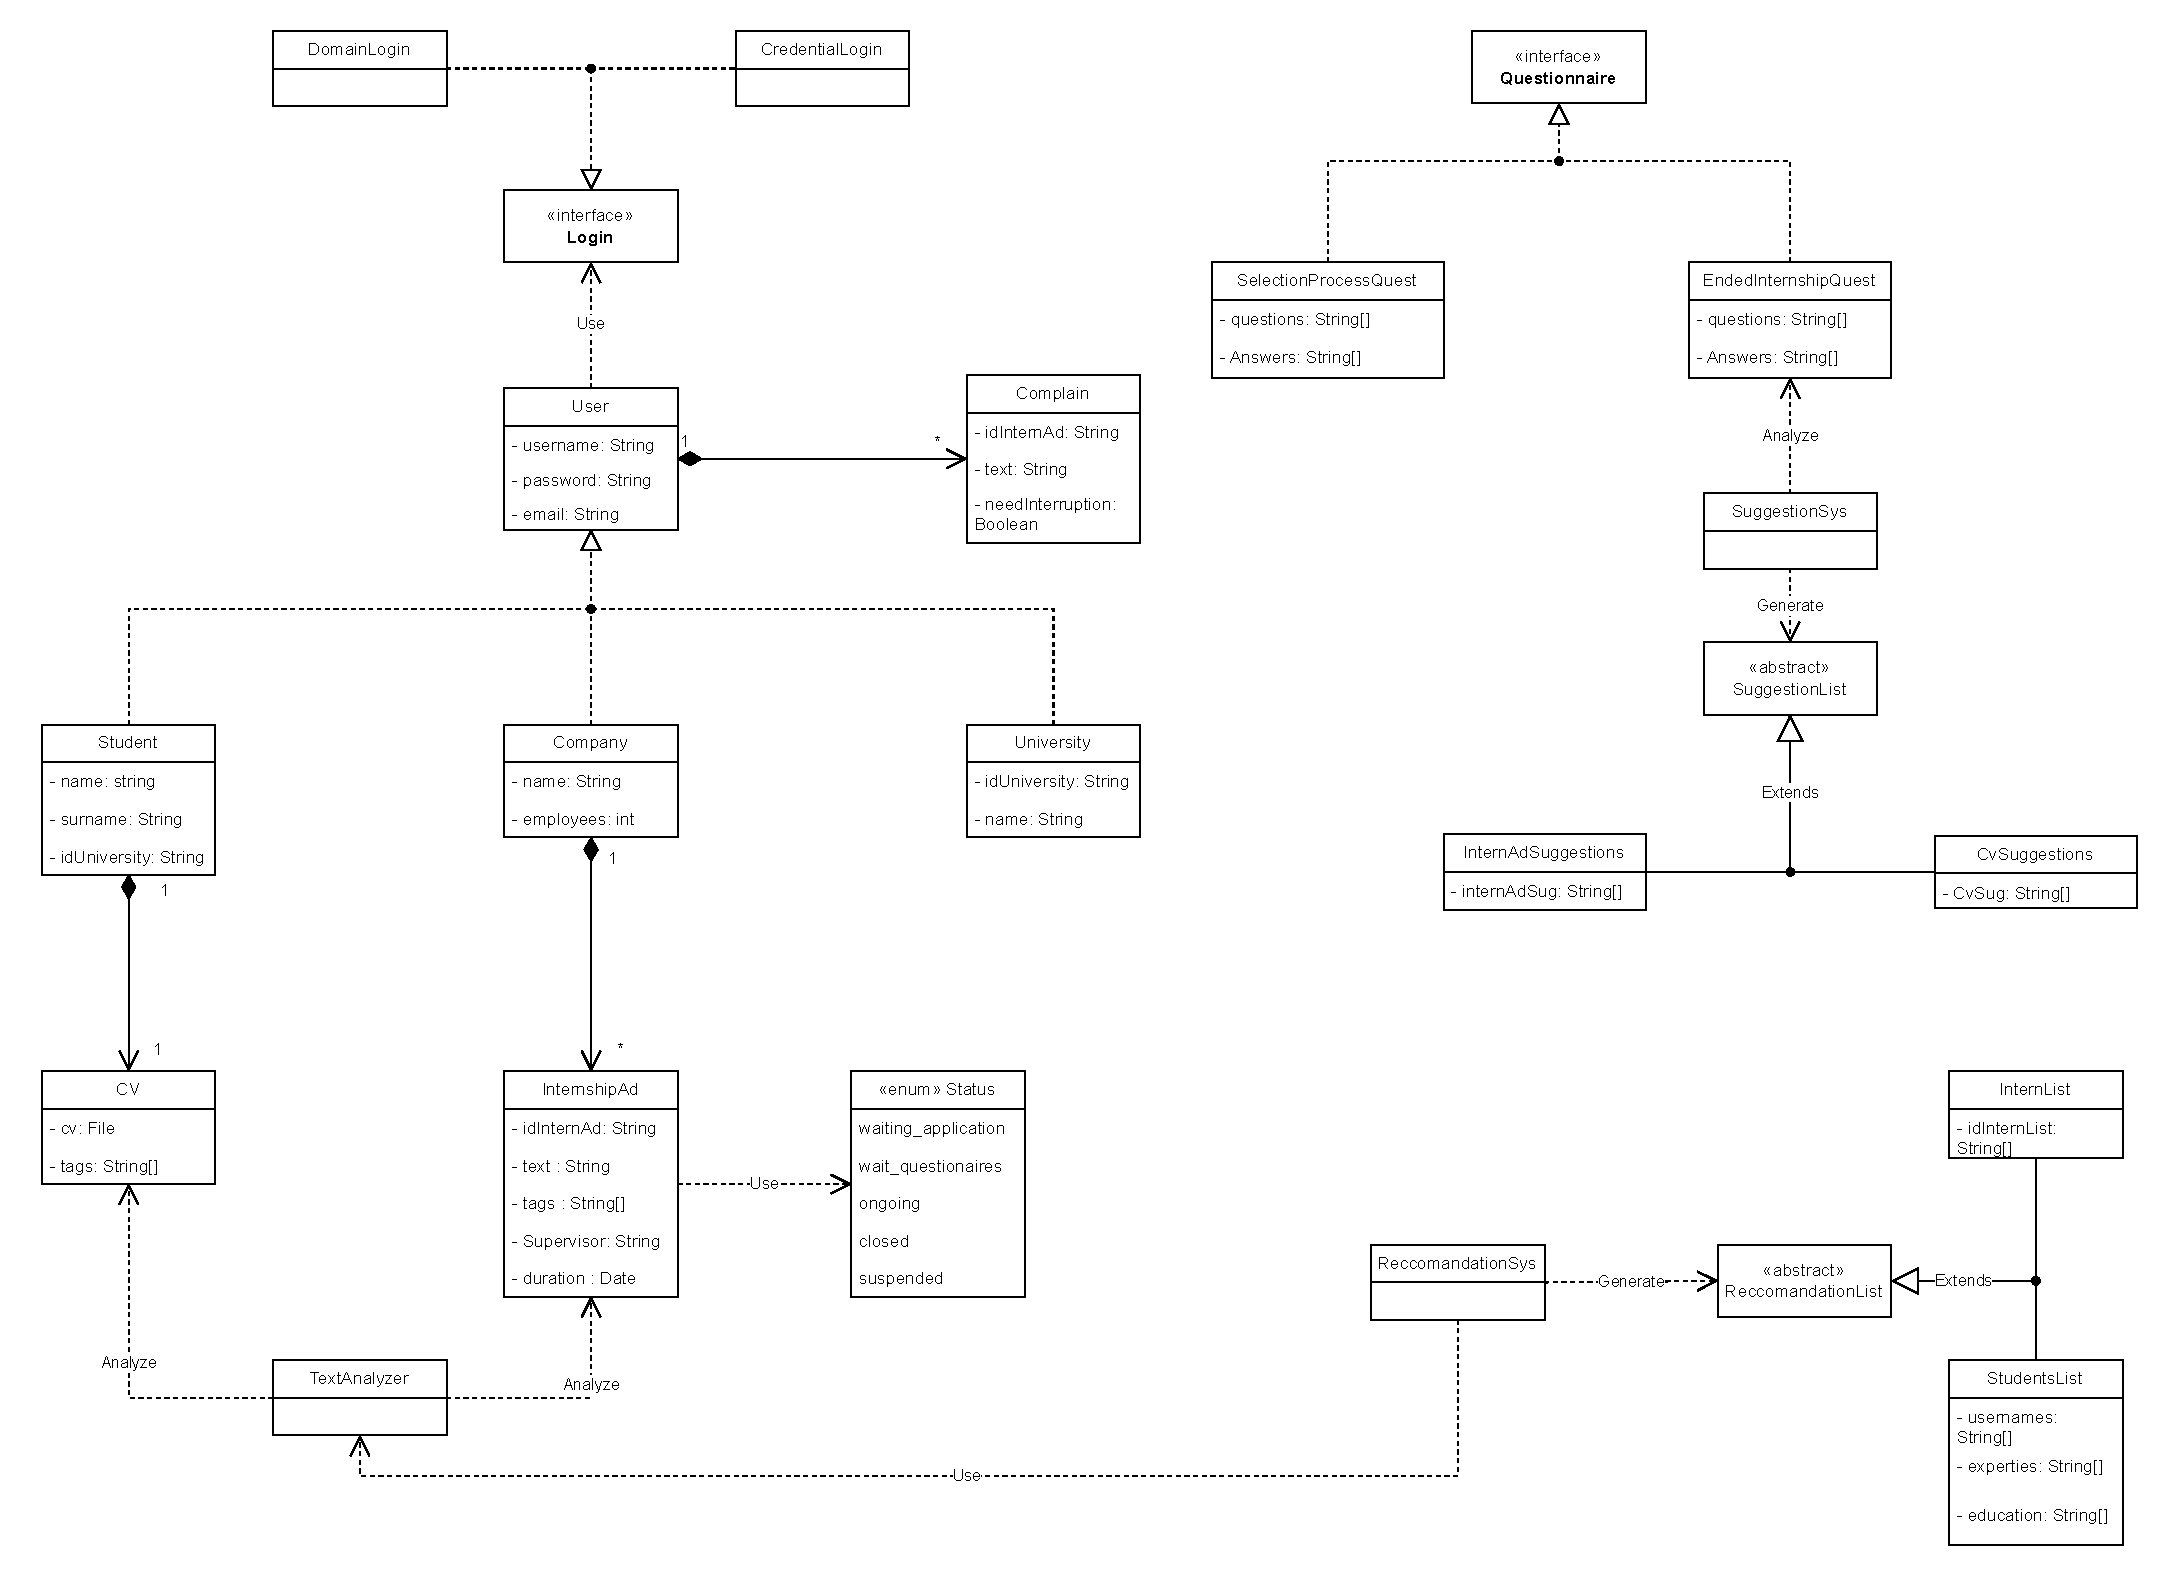
\includegraphics[width=1.0\textwidth]{Images/UML.pdf}
      \caption{High Level View - Class Diagram}
      \label{fig:class_diagram}
\end{figure}

\par The class diagram in figure \ref{fig:class_diagram} shows the high-level structure of the system. The classes of
the system actors, that are Student, Company, and University, are an extension of the User class, which is the base
class for all the users of the system, because all of them share some common attributes, the only difference is that
the password for the students is not set because they do the login through the university SSO.

\par The Student can upload a CV, that is stored in the system. The company can create an internship called
InternshipAd, which is stored in the system with a specific ID. The University can access all the internships and the
feedback of all the students that have it's university id.

\par Another important class is the questionnaire, which is an abstract class that is then extended into the selection
process questionnaire and feedback questionnaire, which are the two types of questionnaires that the system manages.
The first one is created by a CO to select the students for the internship, the second one is created by the system at
the end of the internship to collect feedback from both the student and the company. In this diagram are also
represented the subsystems that will do the analysis of the CVs and the internship ads, to create suggestions to
improve the CVs and the internship ads, and the one that is responsible for the recommendation that the students and
the companies receive by email.

\section{Product Functions}
\label{sec:product_functions}%

\par The following section describes the main functions of the system. The system is divided into three main actors:
the Student, the Company, and the University. Each of them has different functions that they can perform on the system.

\par\textbf{Generic Functionalities}

\begin{itemize}
      % F. 1
      \item \textbf{Account creation with verification}:
            We think that given the context in which S\&C will work there are ways improve on the creation of the
            accounts compared to the standard username, mail and password registration. Our idea is that S\&C will sell
            to both universities and companies the possibility of using the application and creating the accounts
            internally based on sales. For universities, when one university buys the S\&C service it will link its
            Active Directory to the S\&C database. This allows the student to access to S\&C with the university
            credentials. For companies, the account creation is handled internally, and the credentials are given to
            them after the contract is signed. With this mechanism we aim to make the platform more attractive for both
            parties because of the extra guarantees, in terms of verified users, that the account creation holds.

            \begin{figure}[H]
                  \centering
                  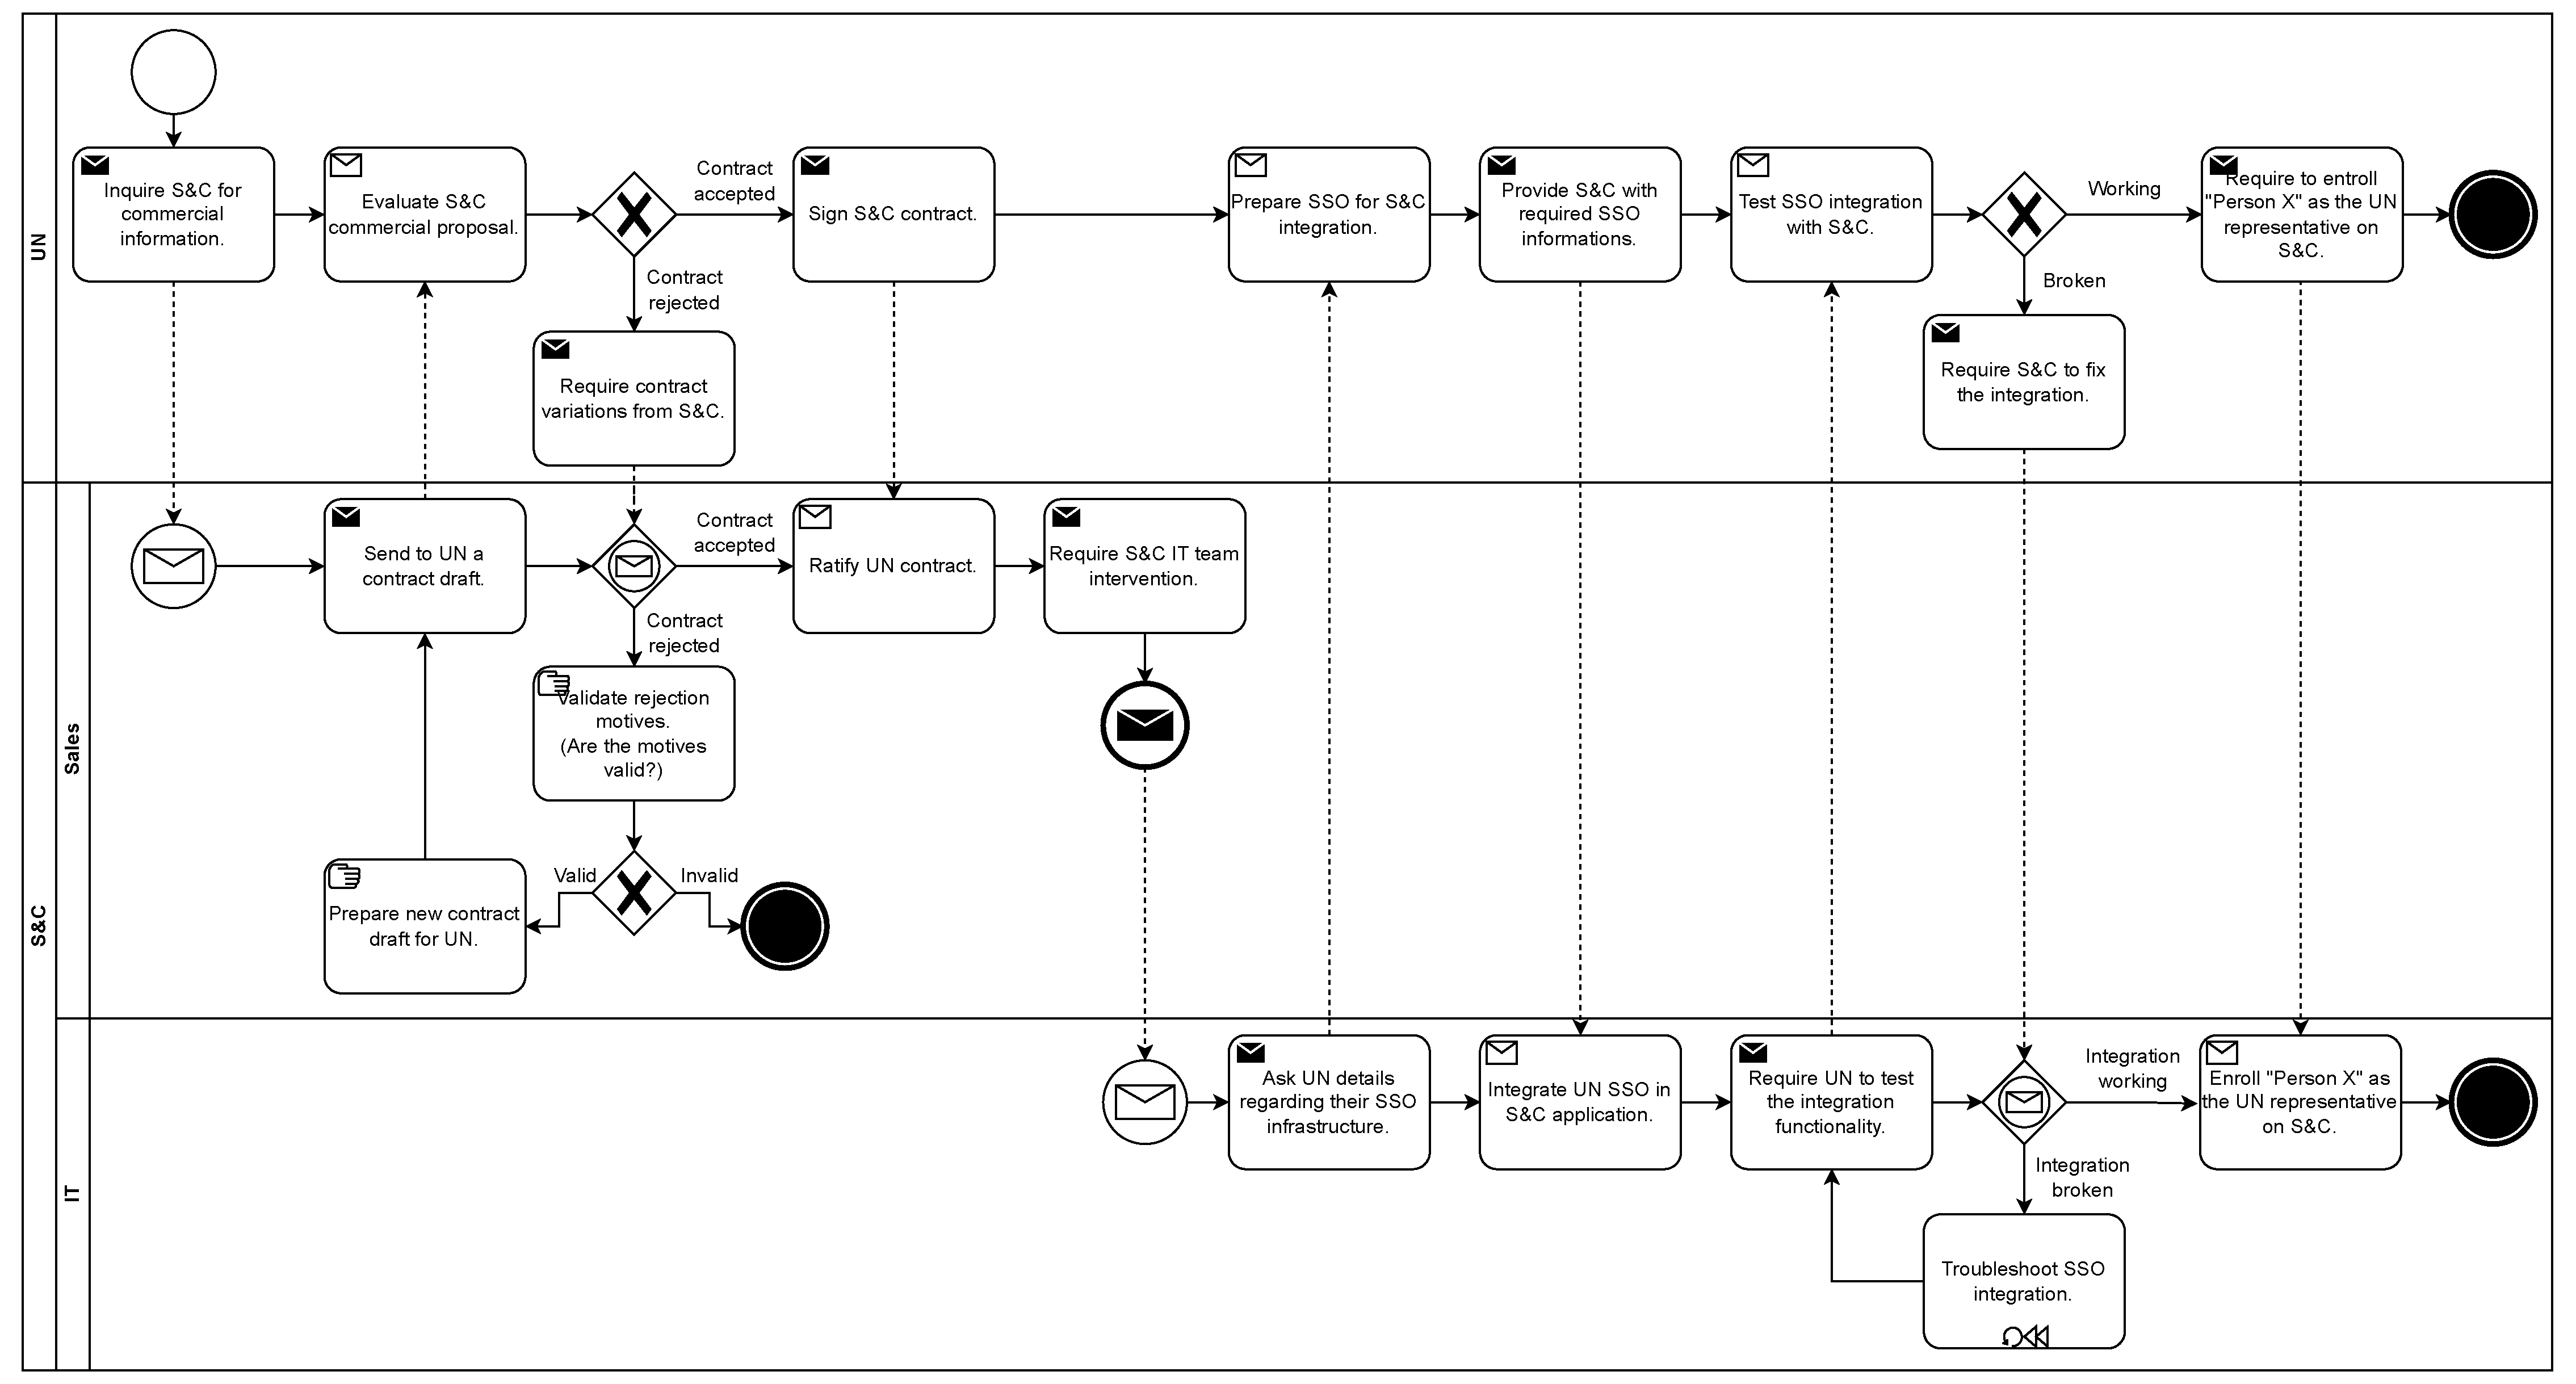
\includegraphics[width=1.0\textwidth]{Images/BPMN_1C.pdf}
                  \caption{UN Enrollment Diagram - Product Function}
                  \label{fig:un_enrollment_diagram}
            \end{figure}

            \begin{figure}[H]
                  \centering
                  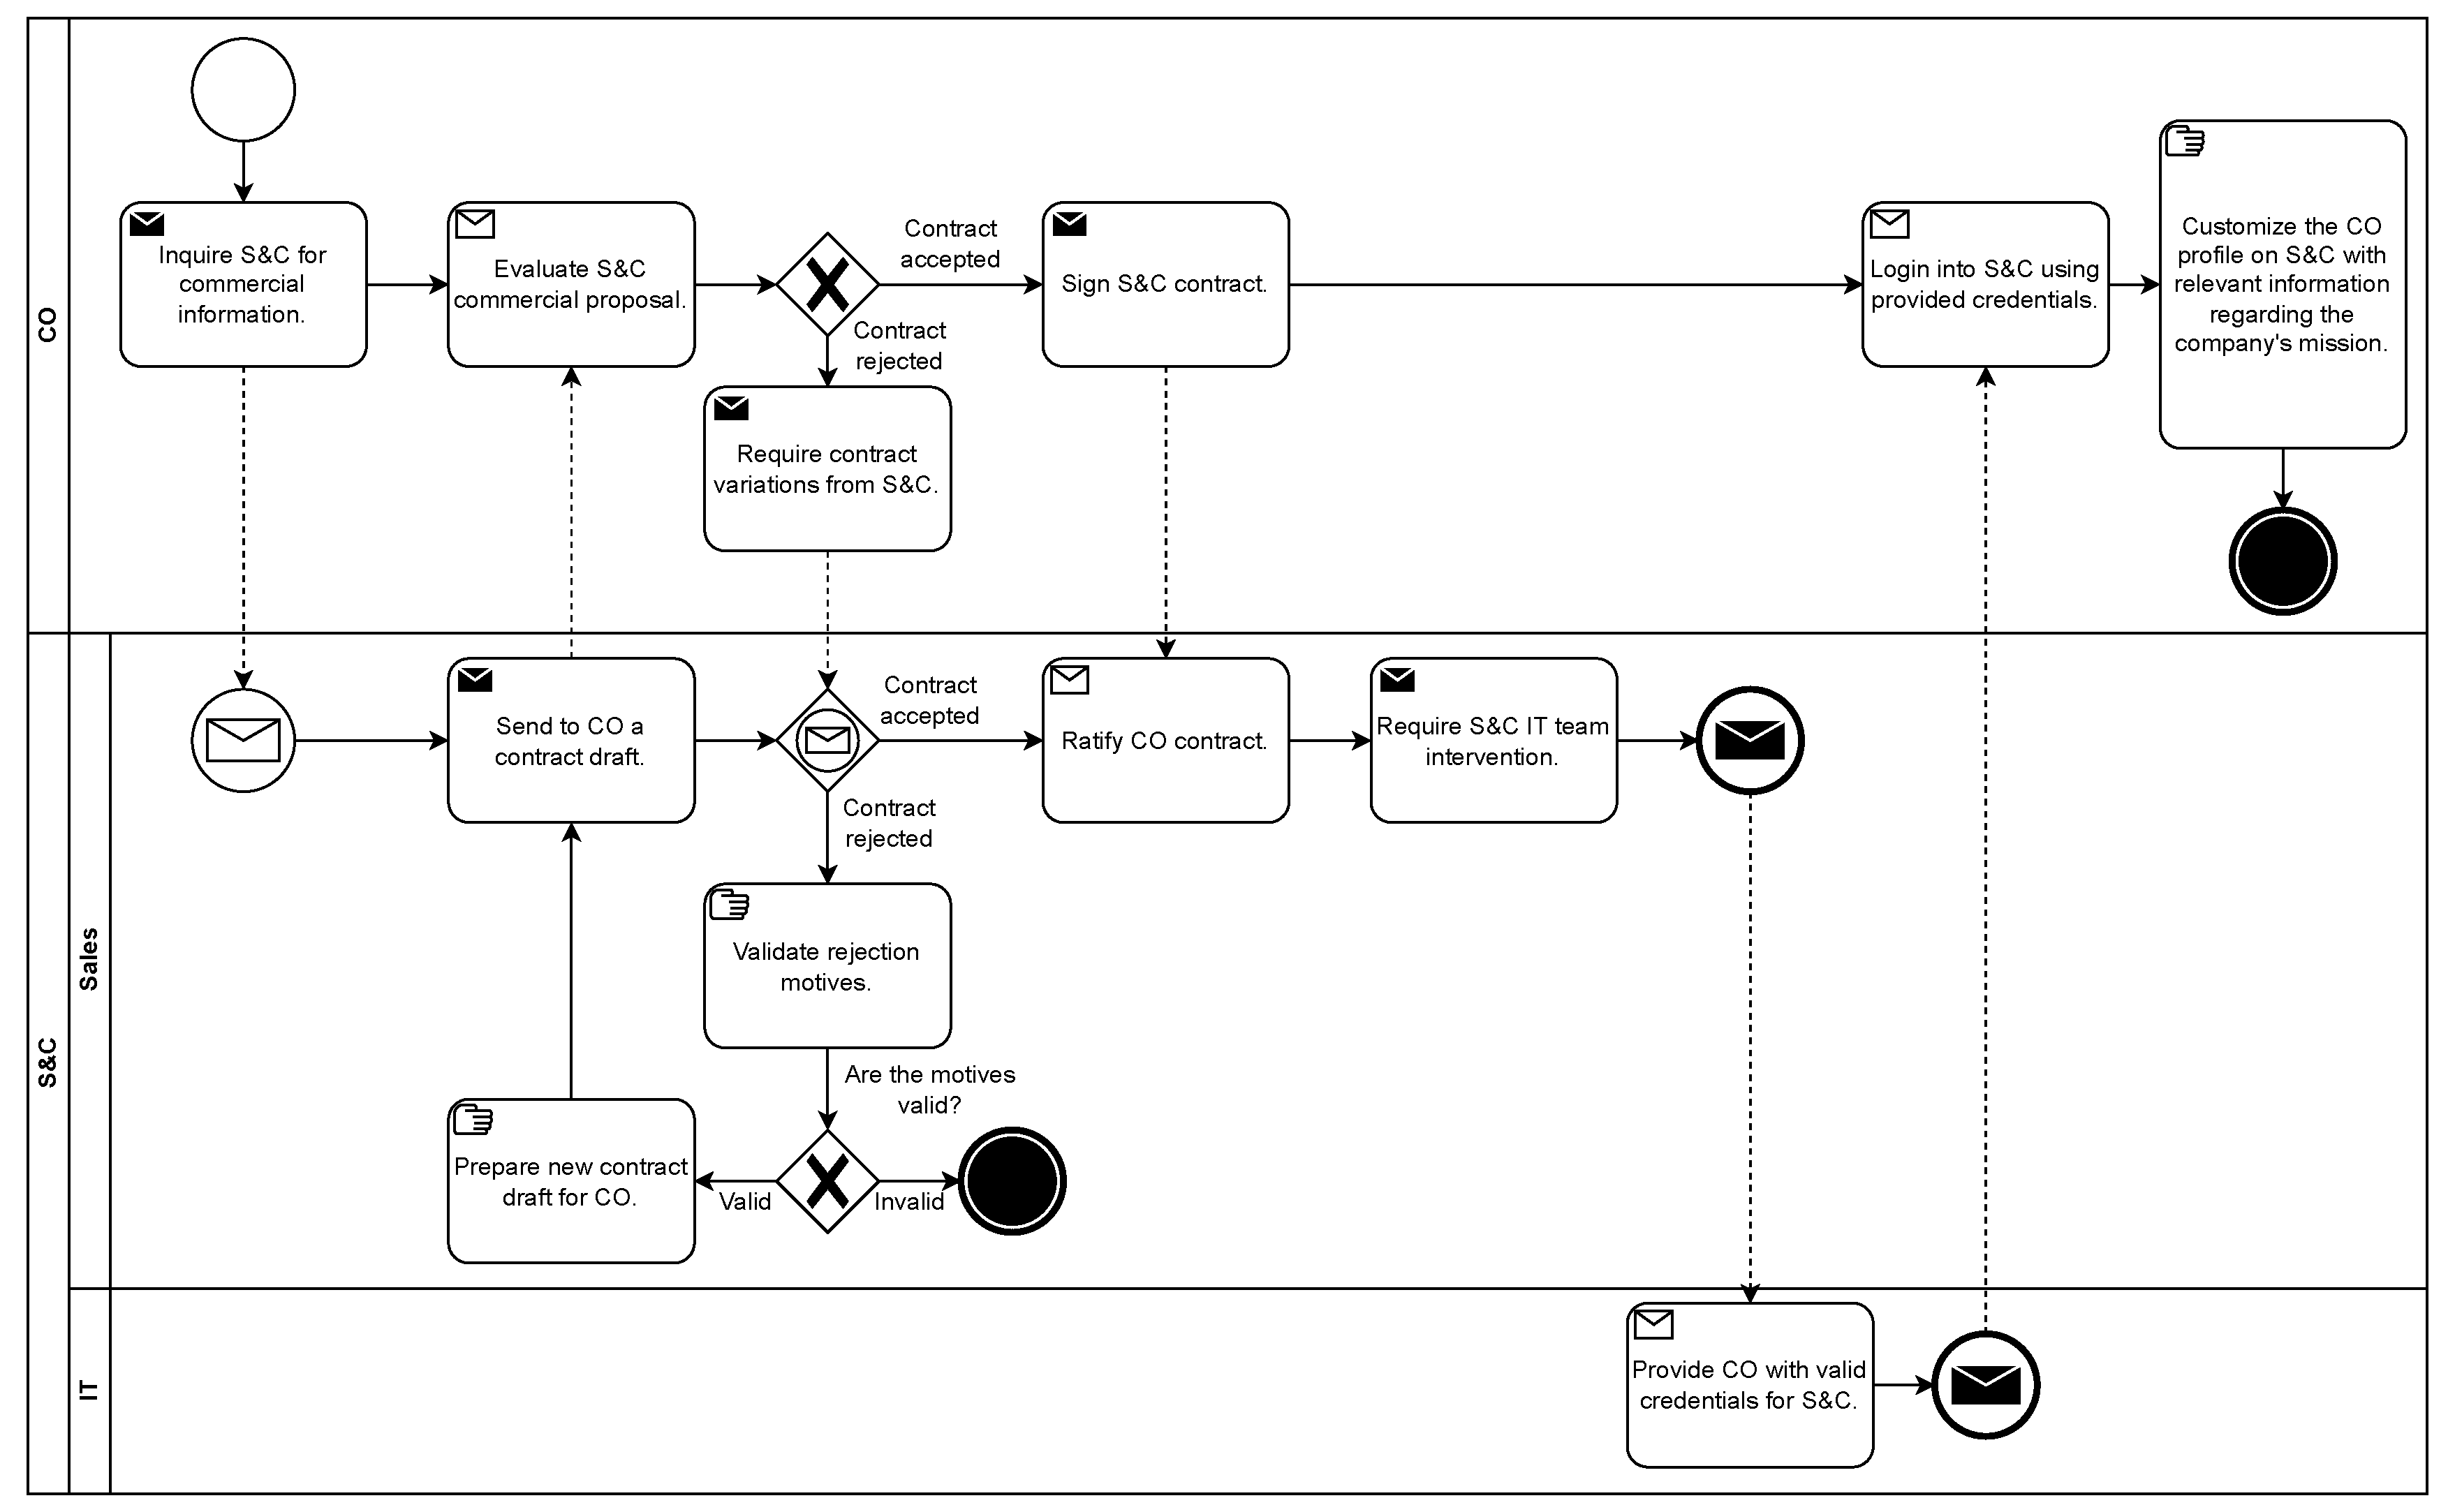
\includegraphics[width=1.0\textwidth]{Images/BPMN_1B.pdf}
                  \caption{CO Enrollment Diagram - Product Function}
                  \label{fig:co_enrollment_diagram}
            \end{figure}

            \begin{figure}[H]
                  \centering
                  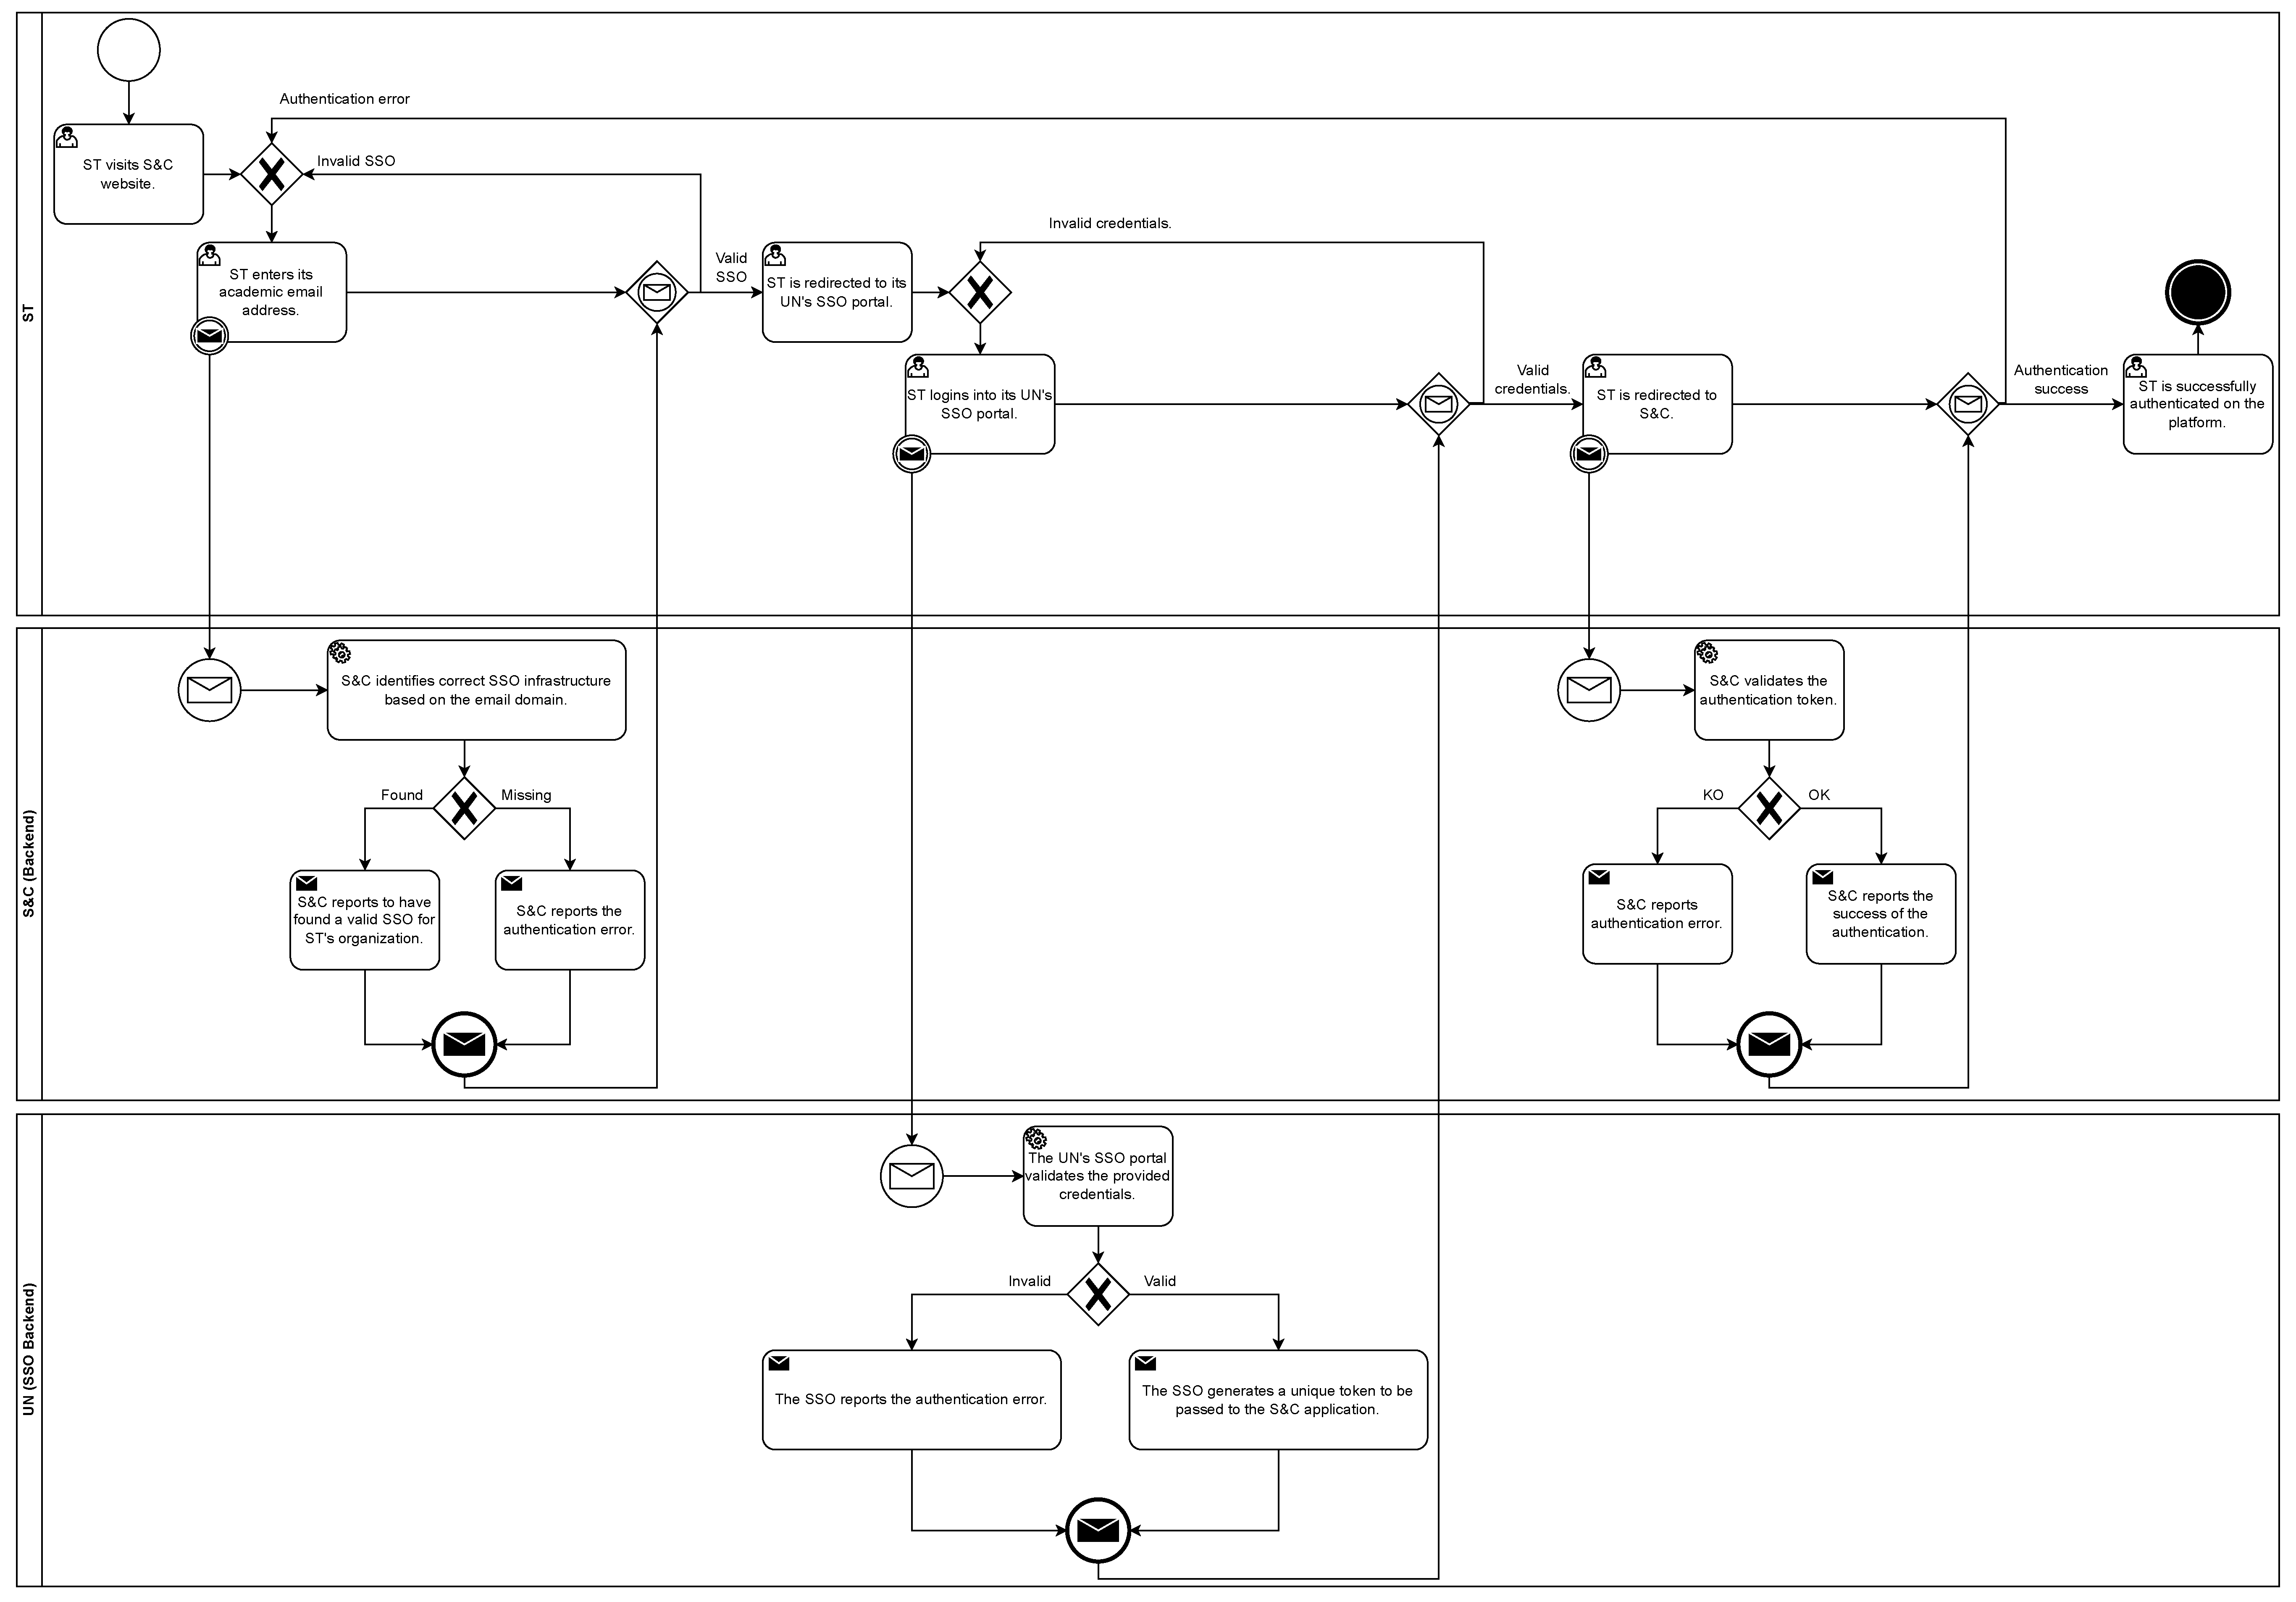
\includegraphics[width=1.0\textwidth]{Images/BPMN_1A.pdf}
                  \caption{ST Enrollment Diagram - Product Function}
                  \label{fig:st_enrollment_diagram}
            \end{figure}

            % F. 2
      \item \textbf{Account improvements suggestions}:
            S\&C offers an improvement guide by providing to both students and companies ideas on how to improve their
            profile / the internships offers to make them more appealing.

            \begin{figure}[H]
                  \centering
                  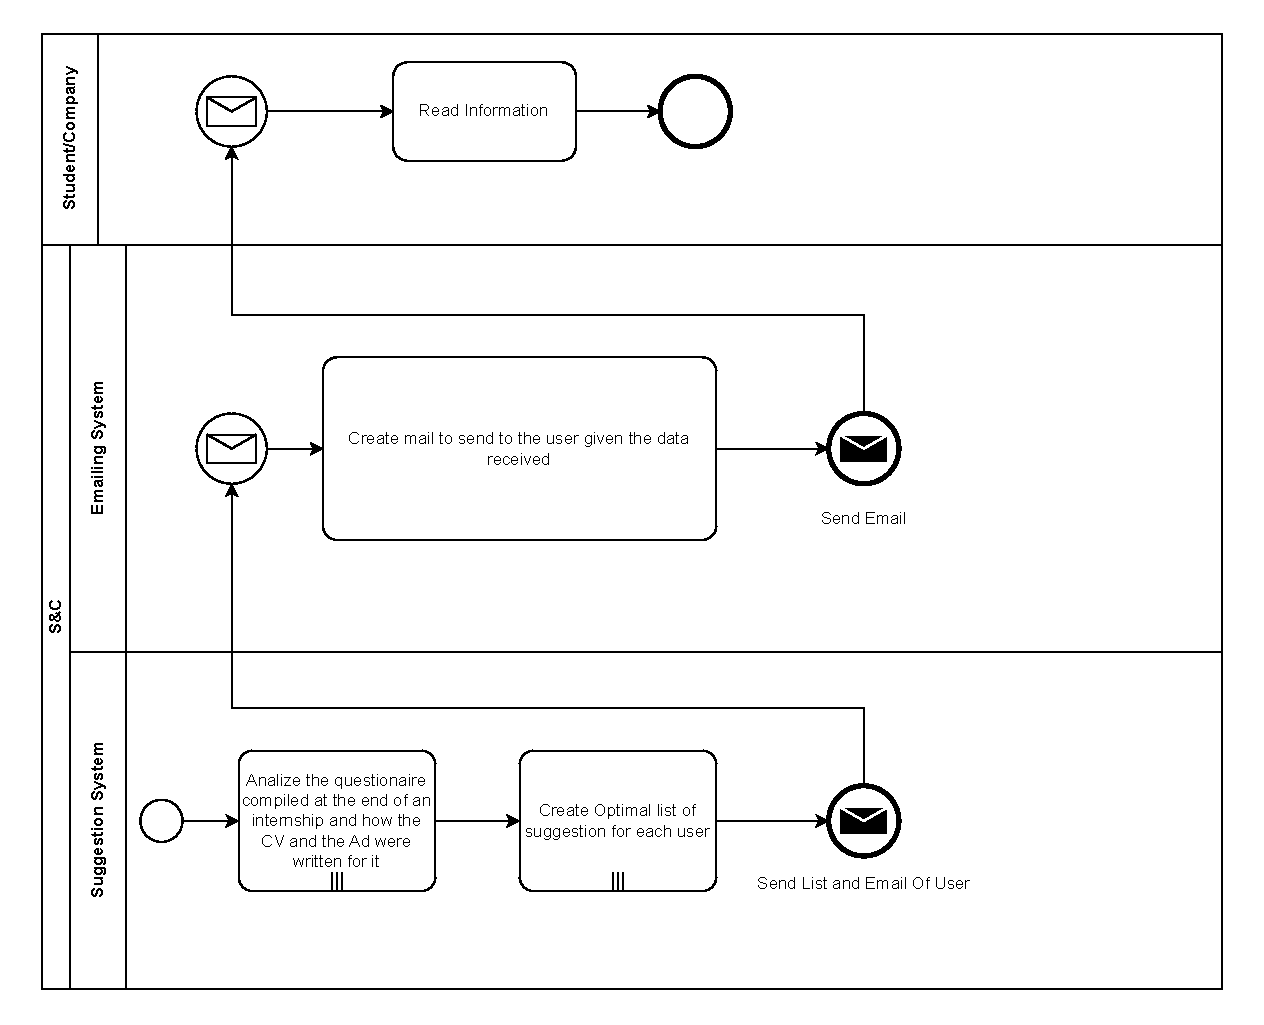
\includegraphics[width=1.0\textwidth]{Images/BPMN_2.pdf}
                  \caption{Account Improvements Suggestions Diagram - Product Function}
                  \label{fig:account_improvements_suggestions_diagram}
            \end{figure}
\end{itemize}

\par\textbf{Student POV Functionalities}

\begin{itemize}
      % F. 3
      \item \textbf{Edit personal data and add extra information}: This includes the possibility to upload/modify the
            CV at any time.

            \begin{figure}[H]
                  \centering
                  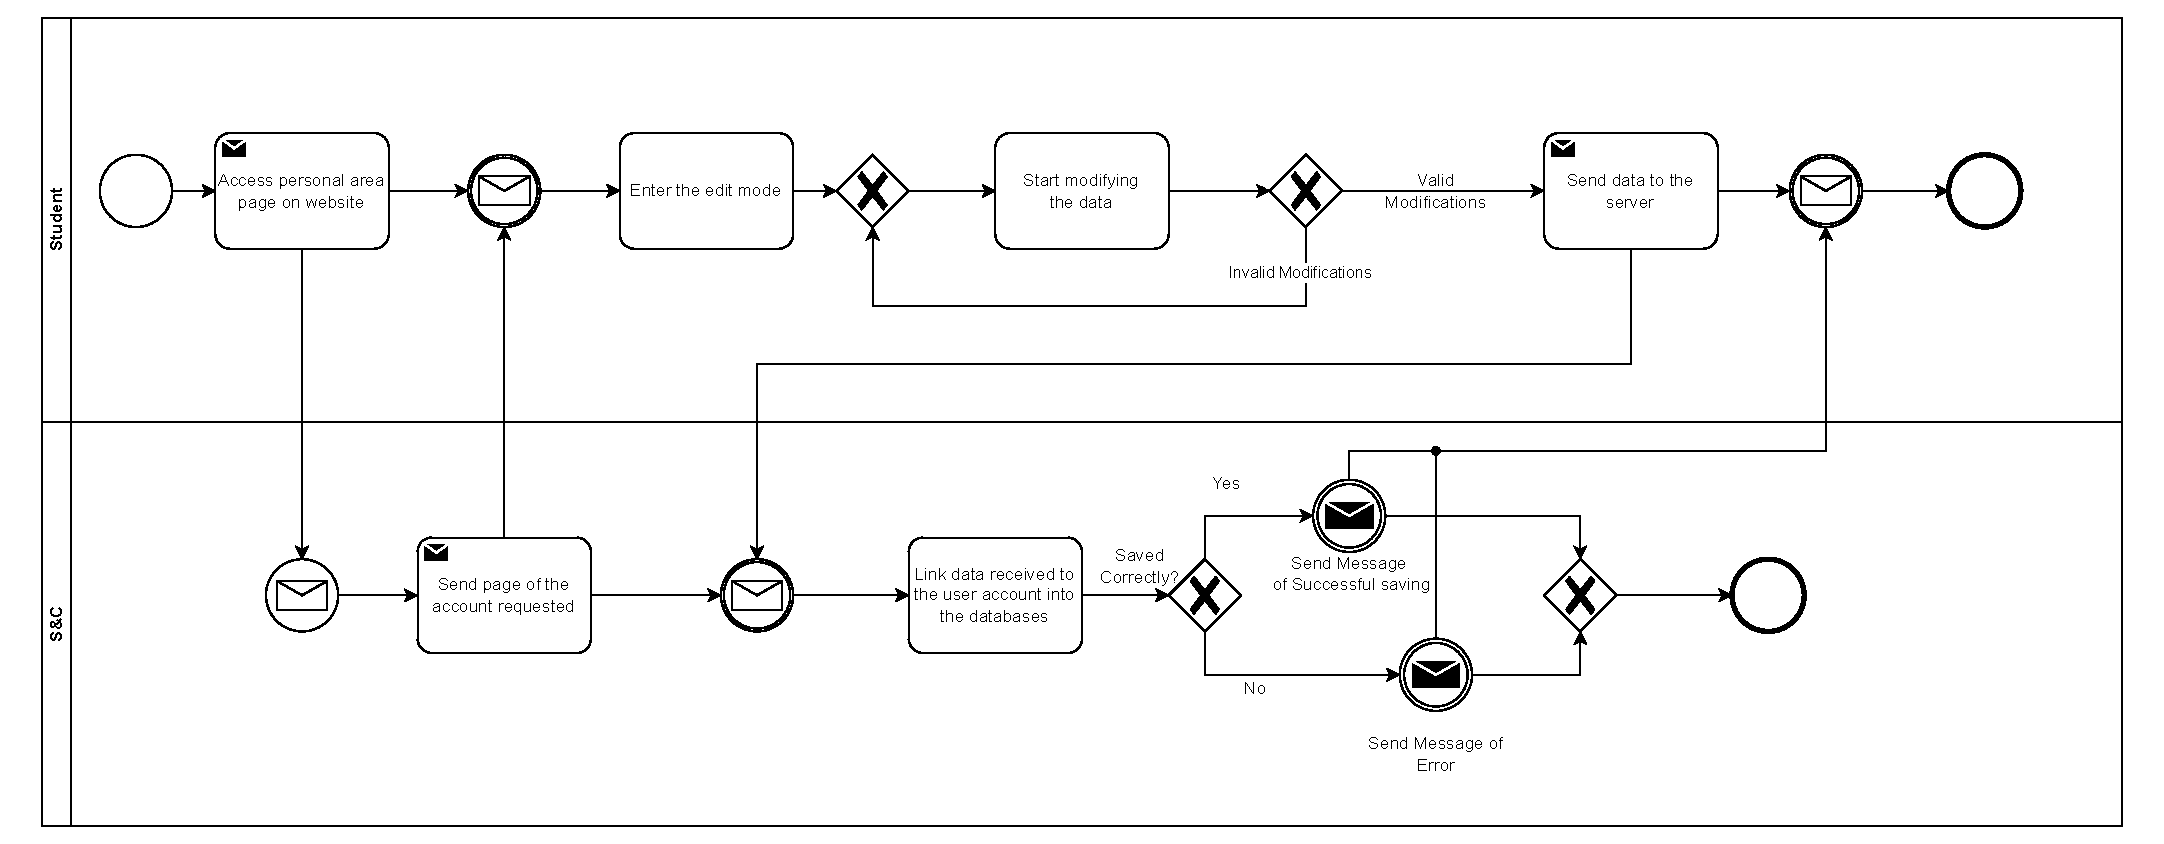
\includegraphics[width=1.0\textwidth]{Images/BPMN_3.pdf}
                  \caption{Edit Personal Data Diagram - Product Function}
                  \label{fig:edit_personal_data_diagram}
            \end{figure}

            % F. 4
      \item \textbf{Search and apply for internship on the app}: This can be conducted by simple keyword search, but
            there are also more advanced search functionalities to better refine the results. This includes advanced
            search filters, and suggestions based on recent searches. Applying for an internship will also activate
            notifications to the user whenever the application gets accepted/rejected and whenever the questionnaire
            (see next point) from the company is available.

            \begin{figure}[H]
                  \centering
                  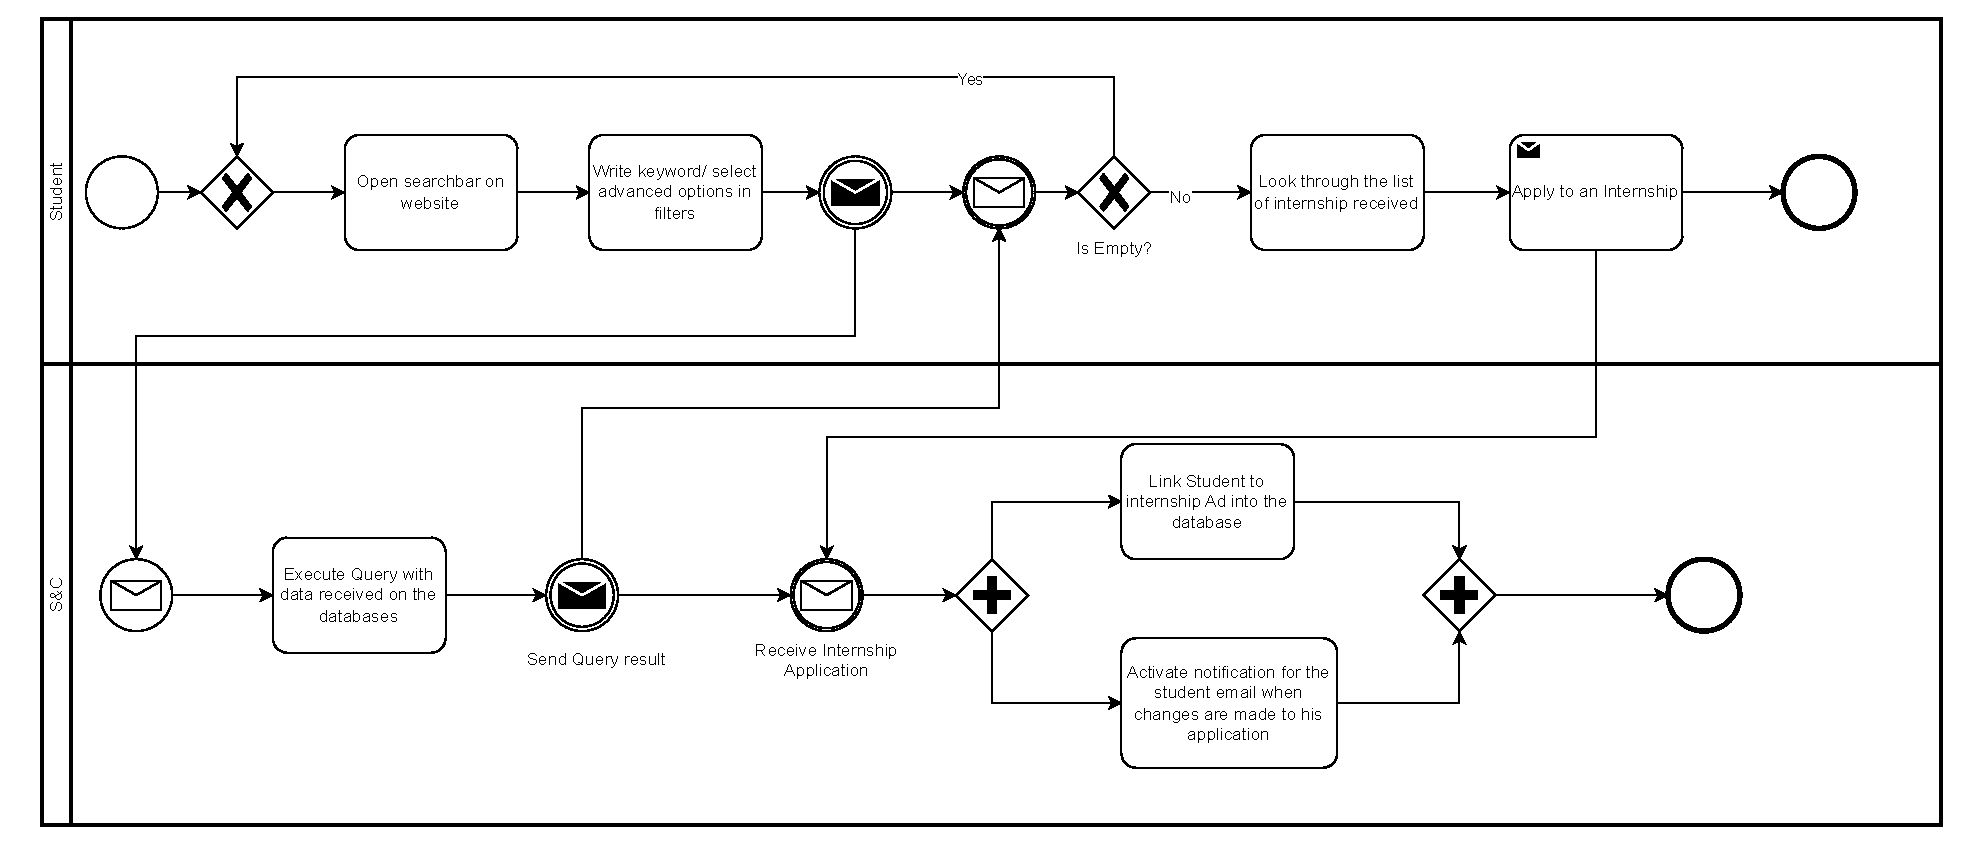
\includegraphics[width=1.0\textwidth]{Images/BPMN_4.pdf}
                  \caption{Search and Apply for Internship Diagram - Product Function}
                  \label{fig:search_and_apply_for_internship_diagram}
            \end{figure}

            % F. 5
      \item \textbf{Compilation of the questionnaire}: The process of selecting students for an internship is carried
            out through questionnaires. S\&C allows students to compile such questionnaire inside the app and maintain
            partial answers between sessions. Whenever the company has gathered all the results and published them a
            notification will alert the user.

            \begin{figure}[H]
                  \centering
                  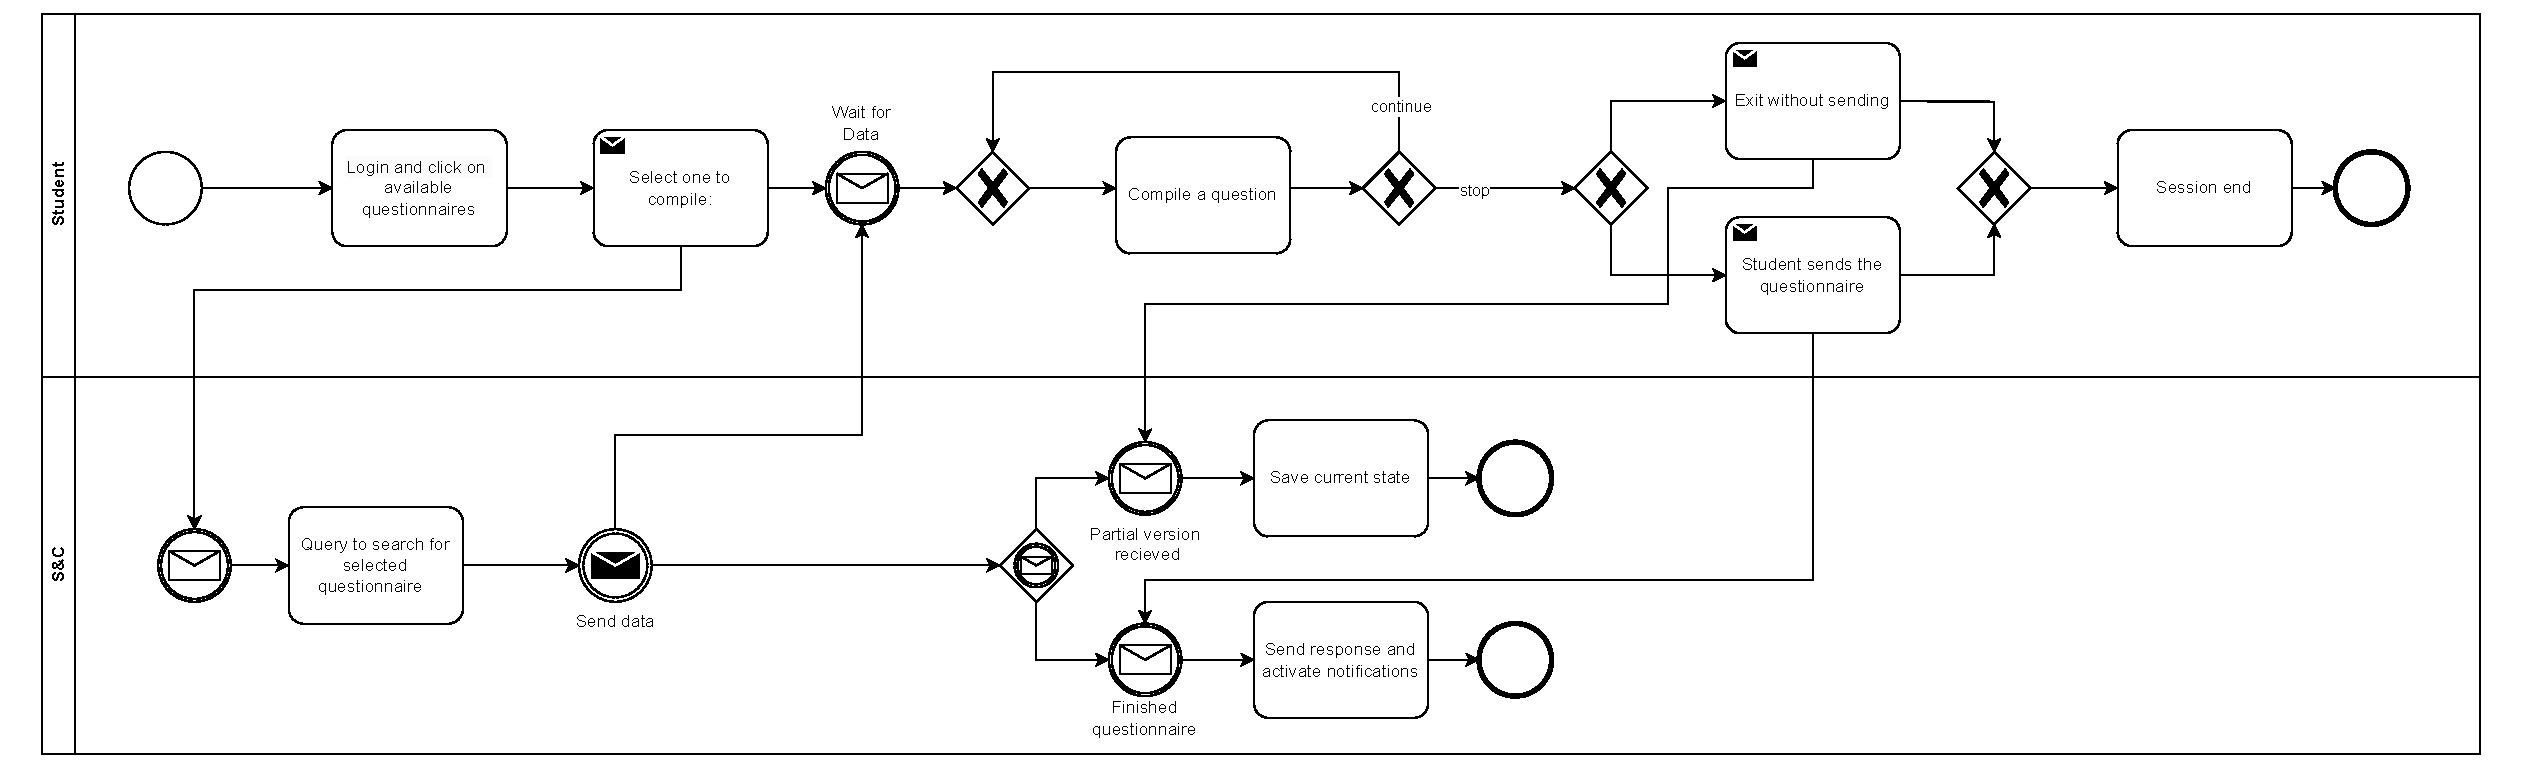
\includegraphics[width=1.0\textwidth]{Images/BPMN_5.pdf}
                  \caption{Compilation of Questionnaire Diagram - Product Function}
                  \label{fig:compilation_of_the_questionnaire_diagram}
            \end{figure}
            % F. 6
      \item \textbf{Profiling/Recommendation}: This is an advanced functionality that allows students to run an
            algorithm on their personal data and extract structured data regarding their user profile. This data allows
            S\&C to find internships that might interest the student with a Data Driven approach. Student will also get
            notifications from S\&C whenever a new internship that might interest the student gets published.

            \begin{figure}[H]
                  \centering
                  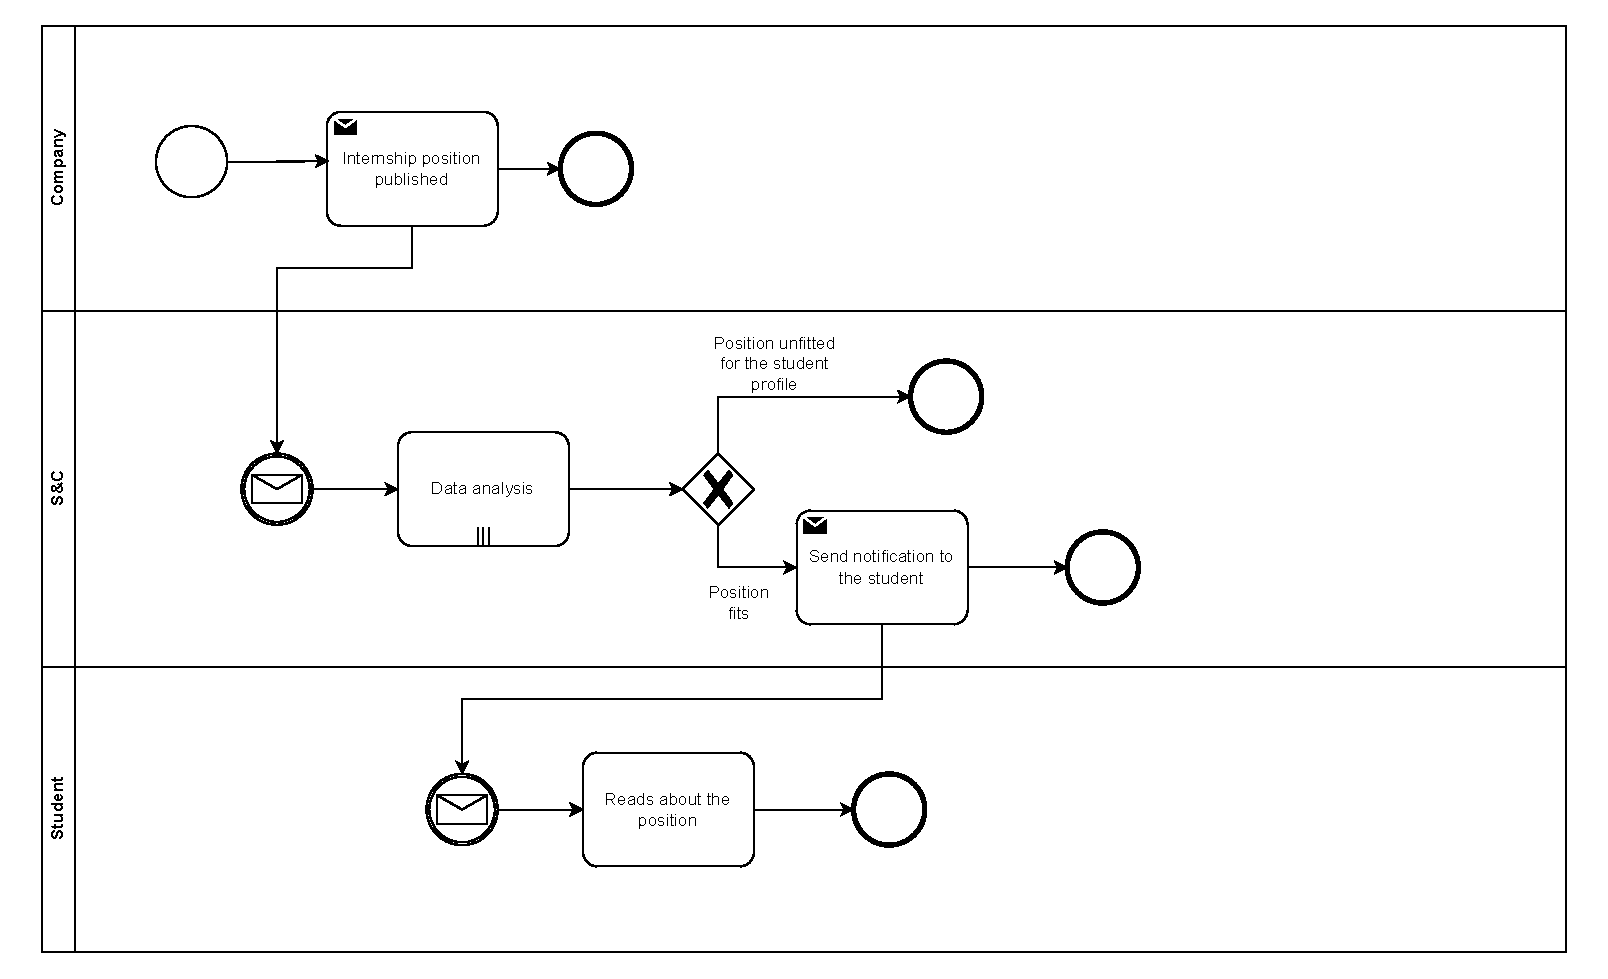
\includegraphics[width=1.0\textwidth]{Images/BPMN_6.pdf}
                  \caption{Profiling/Recommendation Diagram - Product Function}
                  \label{fig:profiling_recommendation_diagram}
            \end{figure}

\end{itemize}

\pagebreak

\par\textbf{Company POV Functionalities}

\begin{itemize}
      % F. 8
      \item \textbf{Edit the company profile}: The company can edit the profile by adding extra descriptive data. The
            aim of this is to allow students to decide where to apply based on the available data. This data also
            supports the suggestion mechanism of S\&C.

            \begin{figure}[H]
                  \centering
                  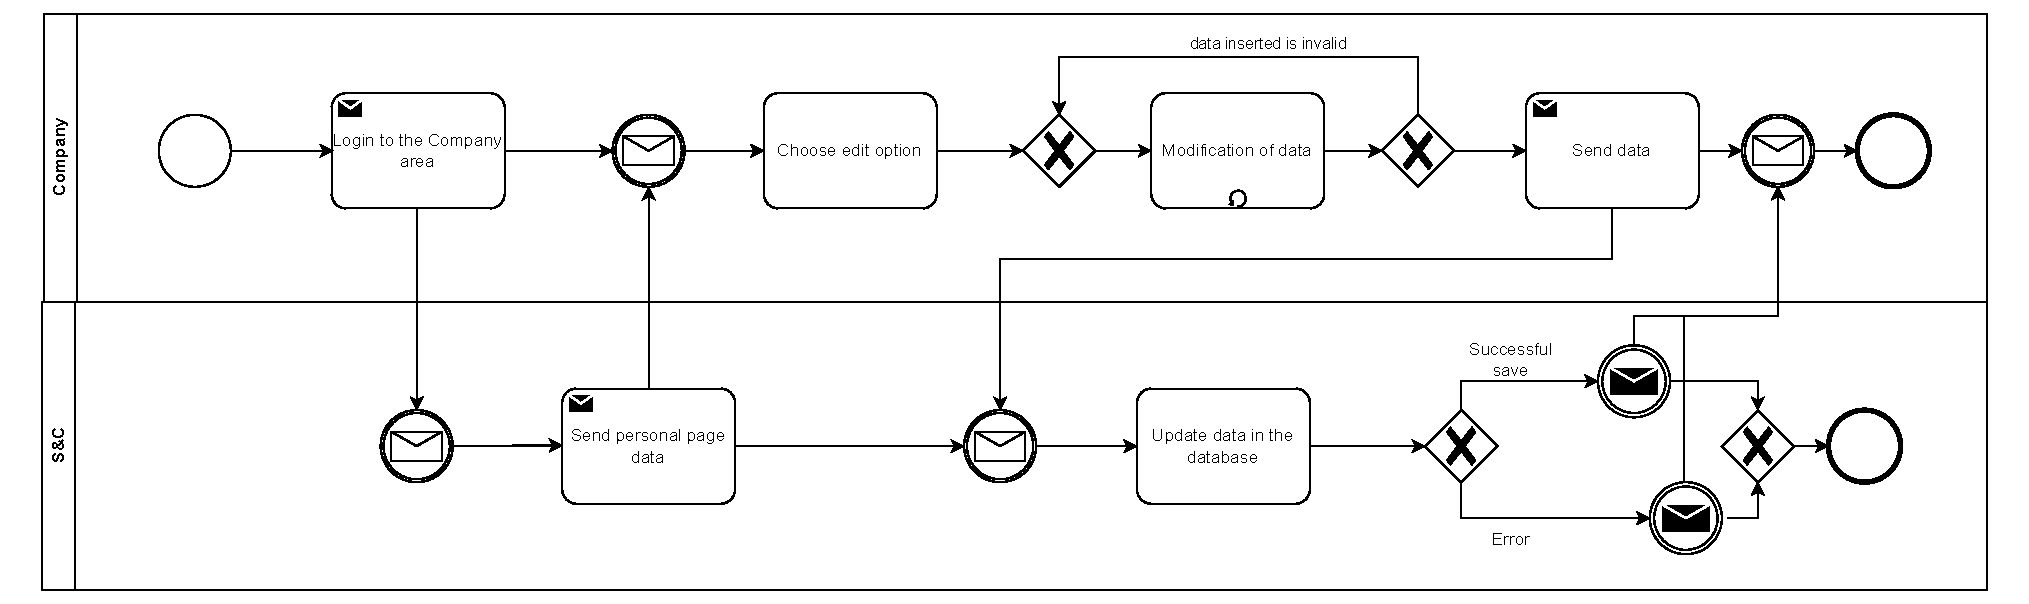
\includegraphics[width=1.0\textwidth]{Images/BPMN_8.pdf}
                  \caption{Edit the CO Profile Diagram - Product Function}
                  \label{fig:edit_the_company_profile_diagram}
            \end{figure}

            % F. 9
      \item \textbf{Open an internship position}: The main feature of S\&C is the possibility for the company to
            publish information about open positions and advertise them. Interested students are free to apply to them.
            To publish a position the company needs to provide a comprehensive description of the position to guide
            decisions. This is referred to students but also the recommendation system that will try to match
            internships with students. The company also needs to specify a deadline for applications.

            \begin{figure}[H]
                  \centering
                  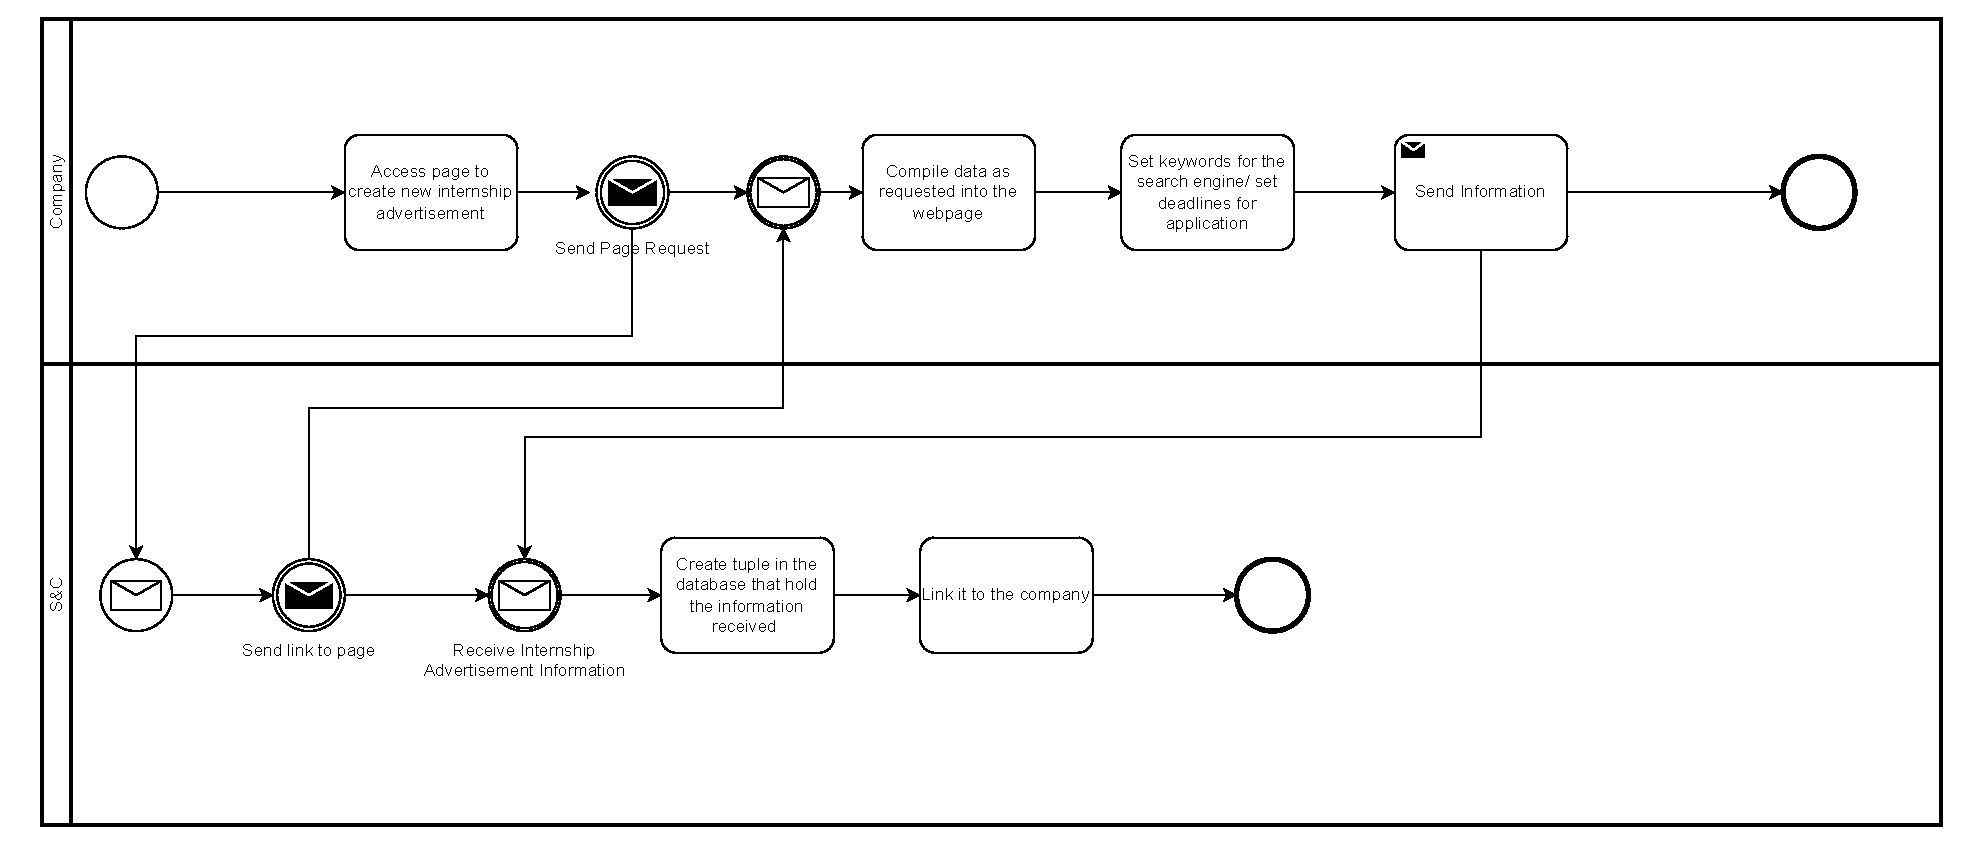
\includegraphics[width=1.0\textwidth]{Images/BPMN_9.pdf}
                  \caption{Open an Internship Position Diagram - Product Function}
                  \label{fig:open_an_internship_position_diagram}
            \end{figure}

            % F. 10
      \item \textbf{Search suitable students}: The recommendation system previously described in the student section
            works also for companies but with some differences. For privacy reasons companies will see the matched
            students data in an anonymous way. With this feature, companies can invite suitable students to take part
            in the selection process. To gain access to more information about the student, including contact
            information, the selection process must go through, this means the student must take the questionnaire and
            get selected.

            \begin{figure}[H]
                  \centering
                  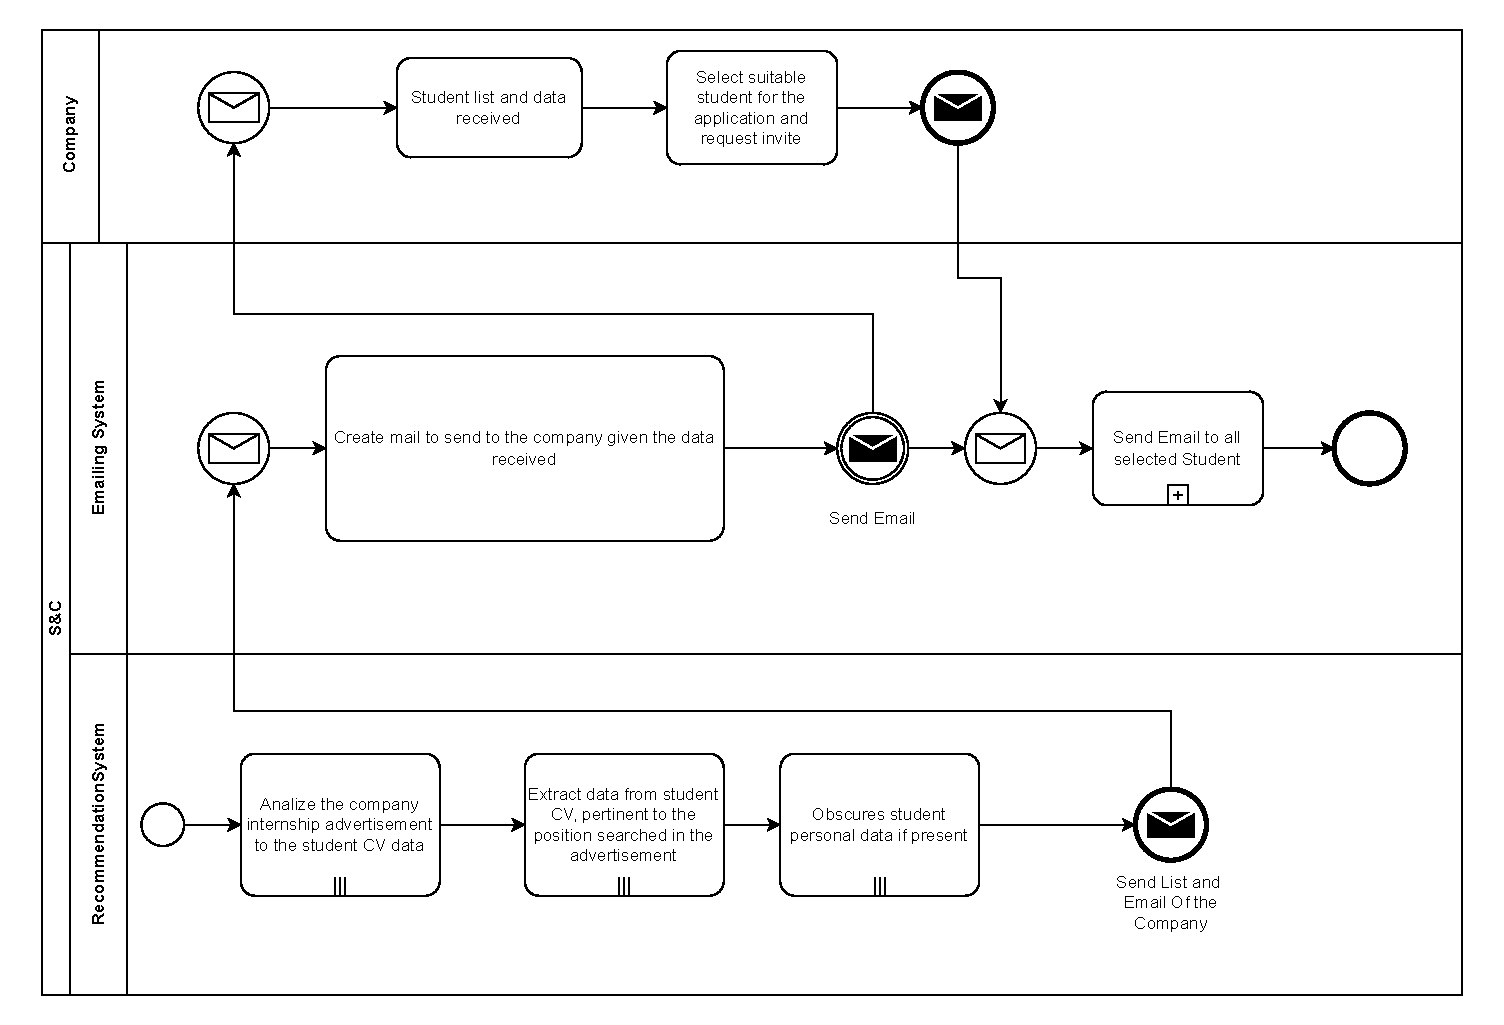
\includegraphics[width=1.0\textwidth]{Images/BPMN_10.pdf}
                  \caption{Search Suitable STs Diagram - Product Function}
                  \label{fig:search_suitable_students_diagram}
            \end{figure}

            % F. 11
      \item \textbf{Create and post personalized questionnaires for the selection phase}: S\&C allows creating and
            customizing questionnaires inside the application to later give them to students as part of the selection
            process. The S\&C application also gathers the answers provided by the students and allows viewing them in
            a structured manner so that the company can easily filter/sort/analyze them and choose the candidates.

            \begin{figure}[H]
                  \centering
                  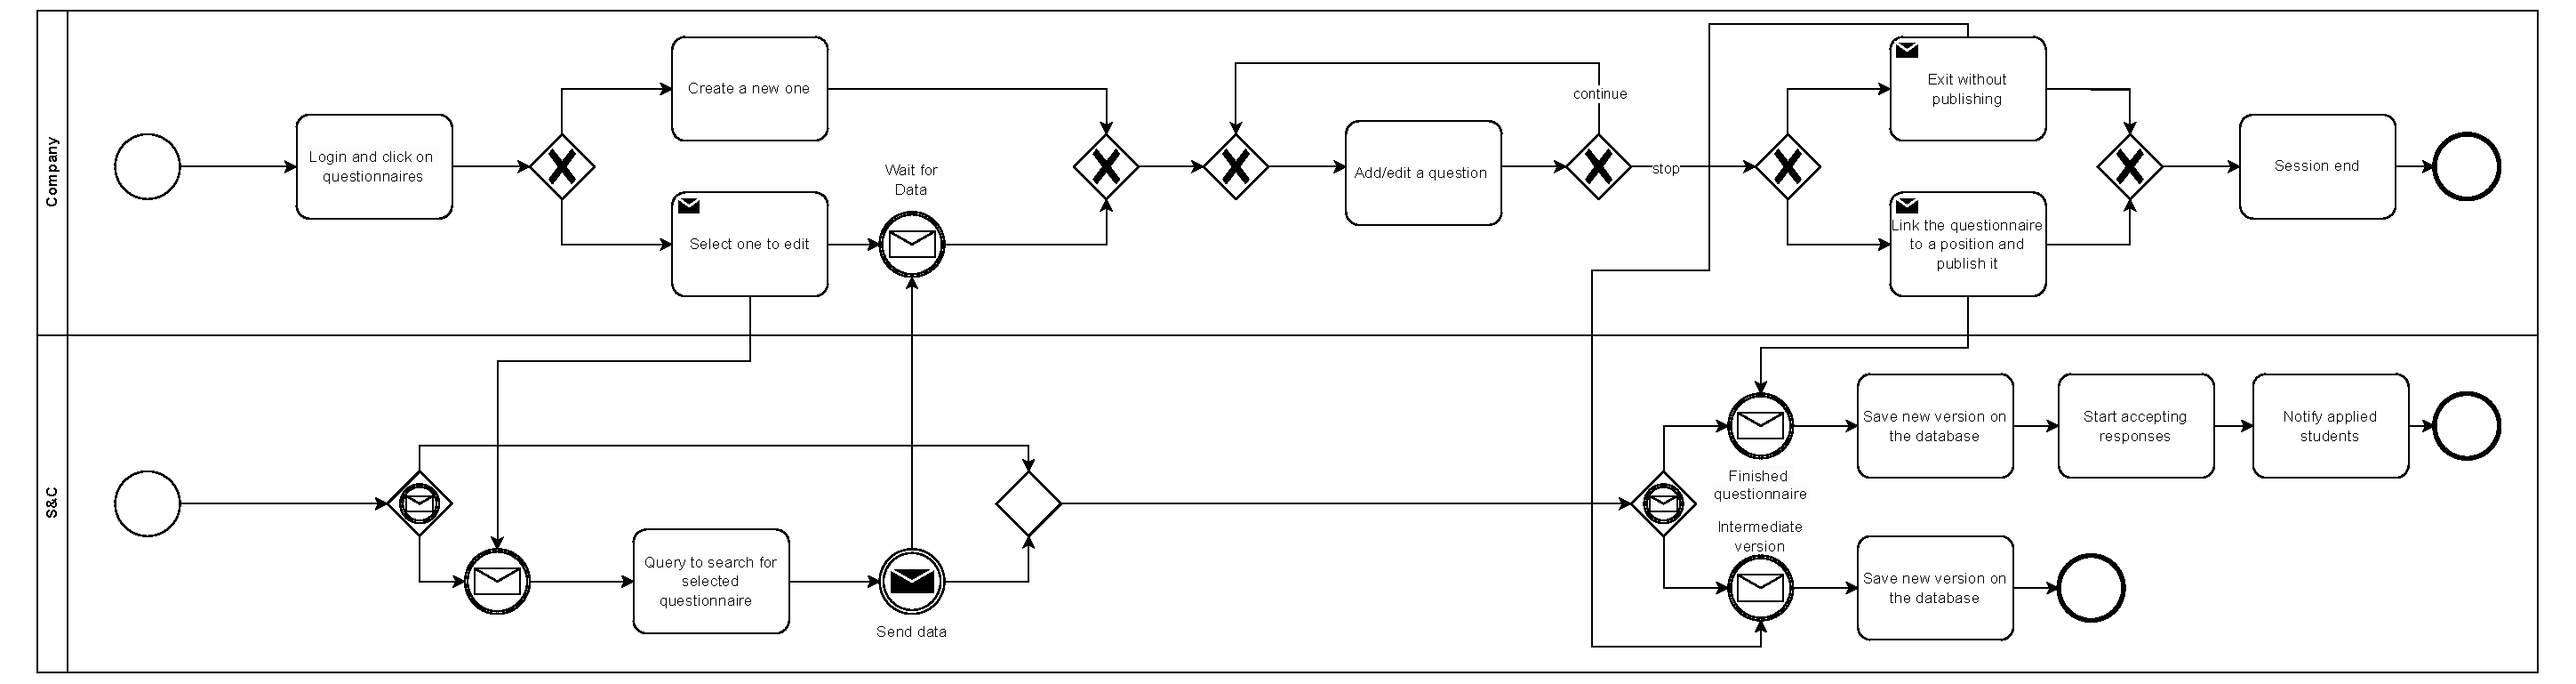
\includegraphics[width=1.0\textwidth]{Images/BPMN_11.pdf}
                  \caption{Create and Post Personalized Questionnaires for the Selection Phase Diagram - Product Function}
                  \label{fig:create_and_post_personalized_questionnaires_for_the_selection_phase_diagram}
            \end{figure}

            % F. 13
      \item \textbf{Monitoring}: This functionality is used by the company to keep track of all the internships
            currently active and monitor how they are going (e.g., if there were complaints, etc.), but also see all
            the past internships for historical data.

            \begin{figure}[H]
                  \centering
                  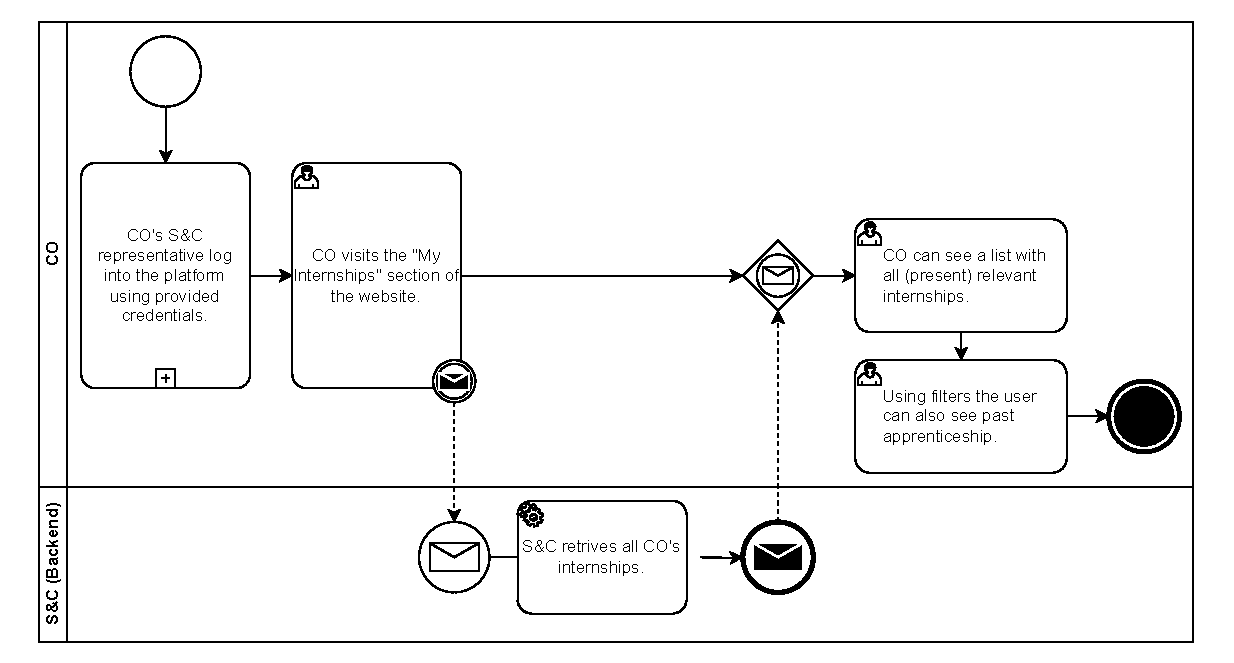
\includegraphics[width=1.0\textwidth]{Images/BPMN_13.pdf}
                  \caption{CO Monitoring Diagram - Product Function}
                  \label{fig:co_monitoring_diagram}
            \end{figure}

\end{itemize}

\par\textbf{University POV Functionalities}

\begin{itemize}
      % F. 14
      \item \textbf{Monitoring}: S\&C keeps track of all the interactions between students and companies (applications
            and internships). The universities can access the portion of this data regarding their own students for
            analysis.

            \begin{figure}[H]
                  \centering
                  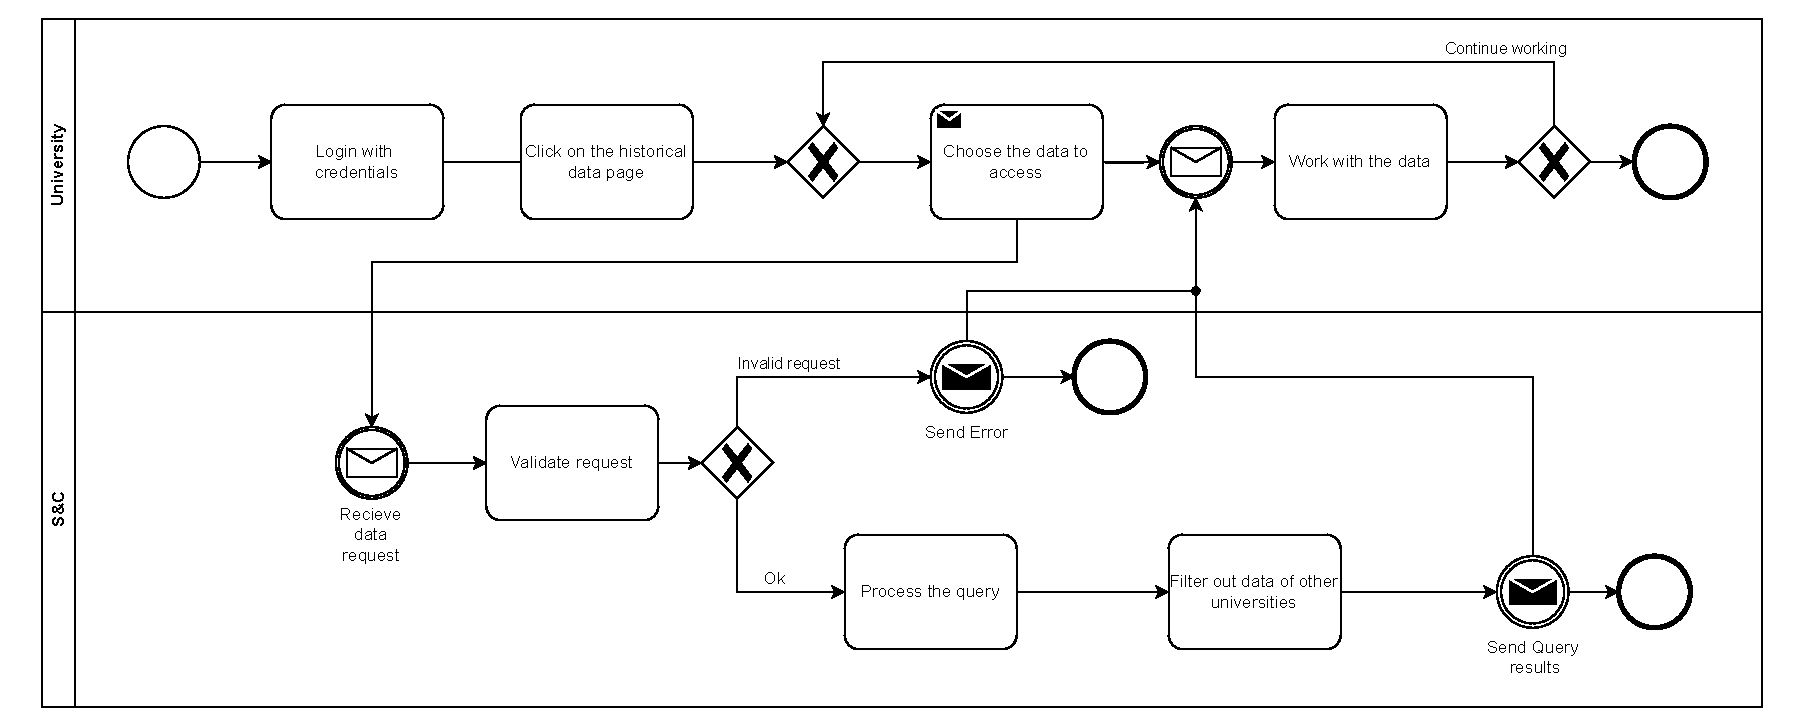
\includegraphics[width=1.0\textwidth]{Images/BPMN_14.pdf}
                  \caption{UN Monitoring Diagram - Product Function}
                  \label{fig:un_monitoring_diagram}
            \end{figure}
            % F. 15
      \item \textbf{Complaint handling}: Universities play an important role in the interaction between students and
            companies during the internship period. If any problem arises during such a period, a student can open a
            complaint ticket. The university steps in to handle the problem by acting as a third party. In the
            worst-case scenario, the suspension or cancellation of the internship is an available option to the
            university.

            \begin{figure}[H]
                  \centering
                  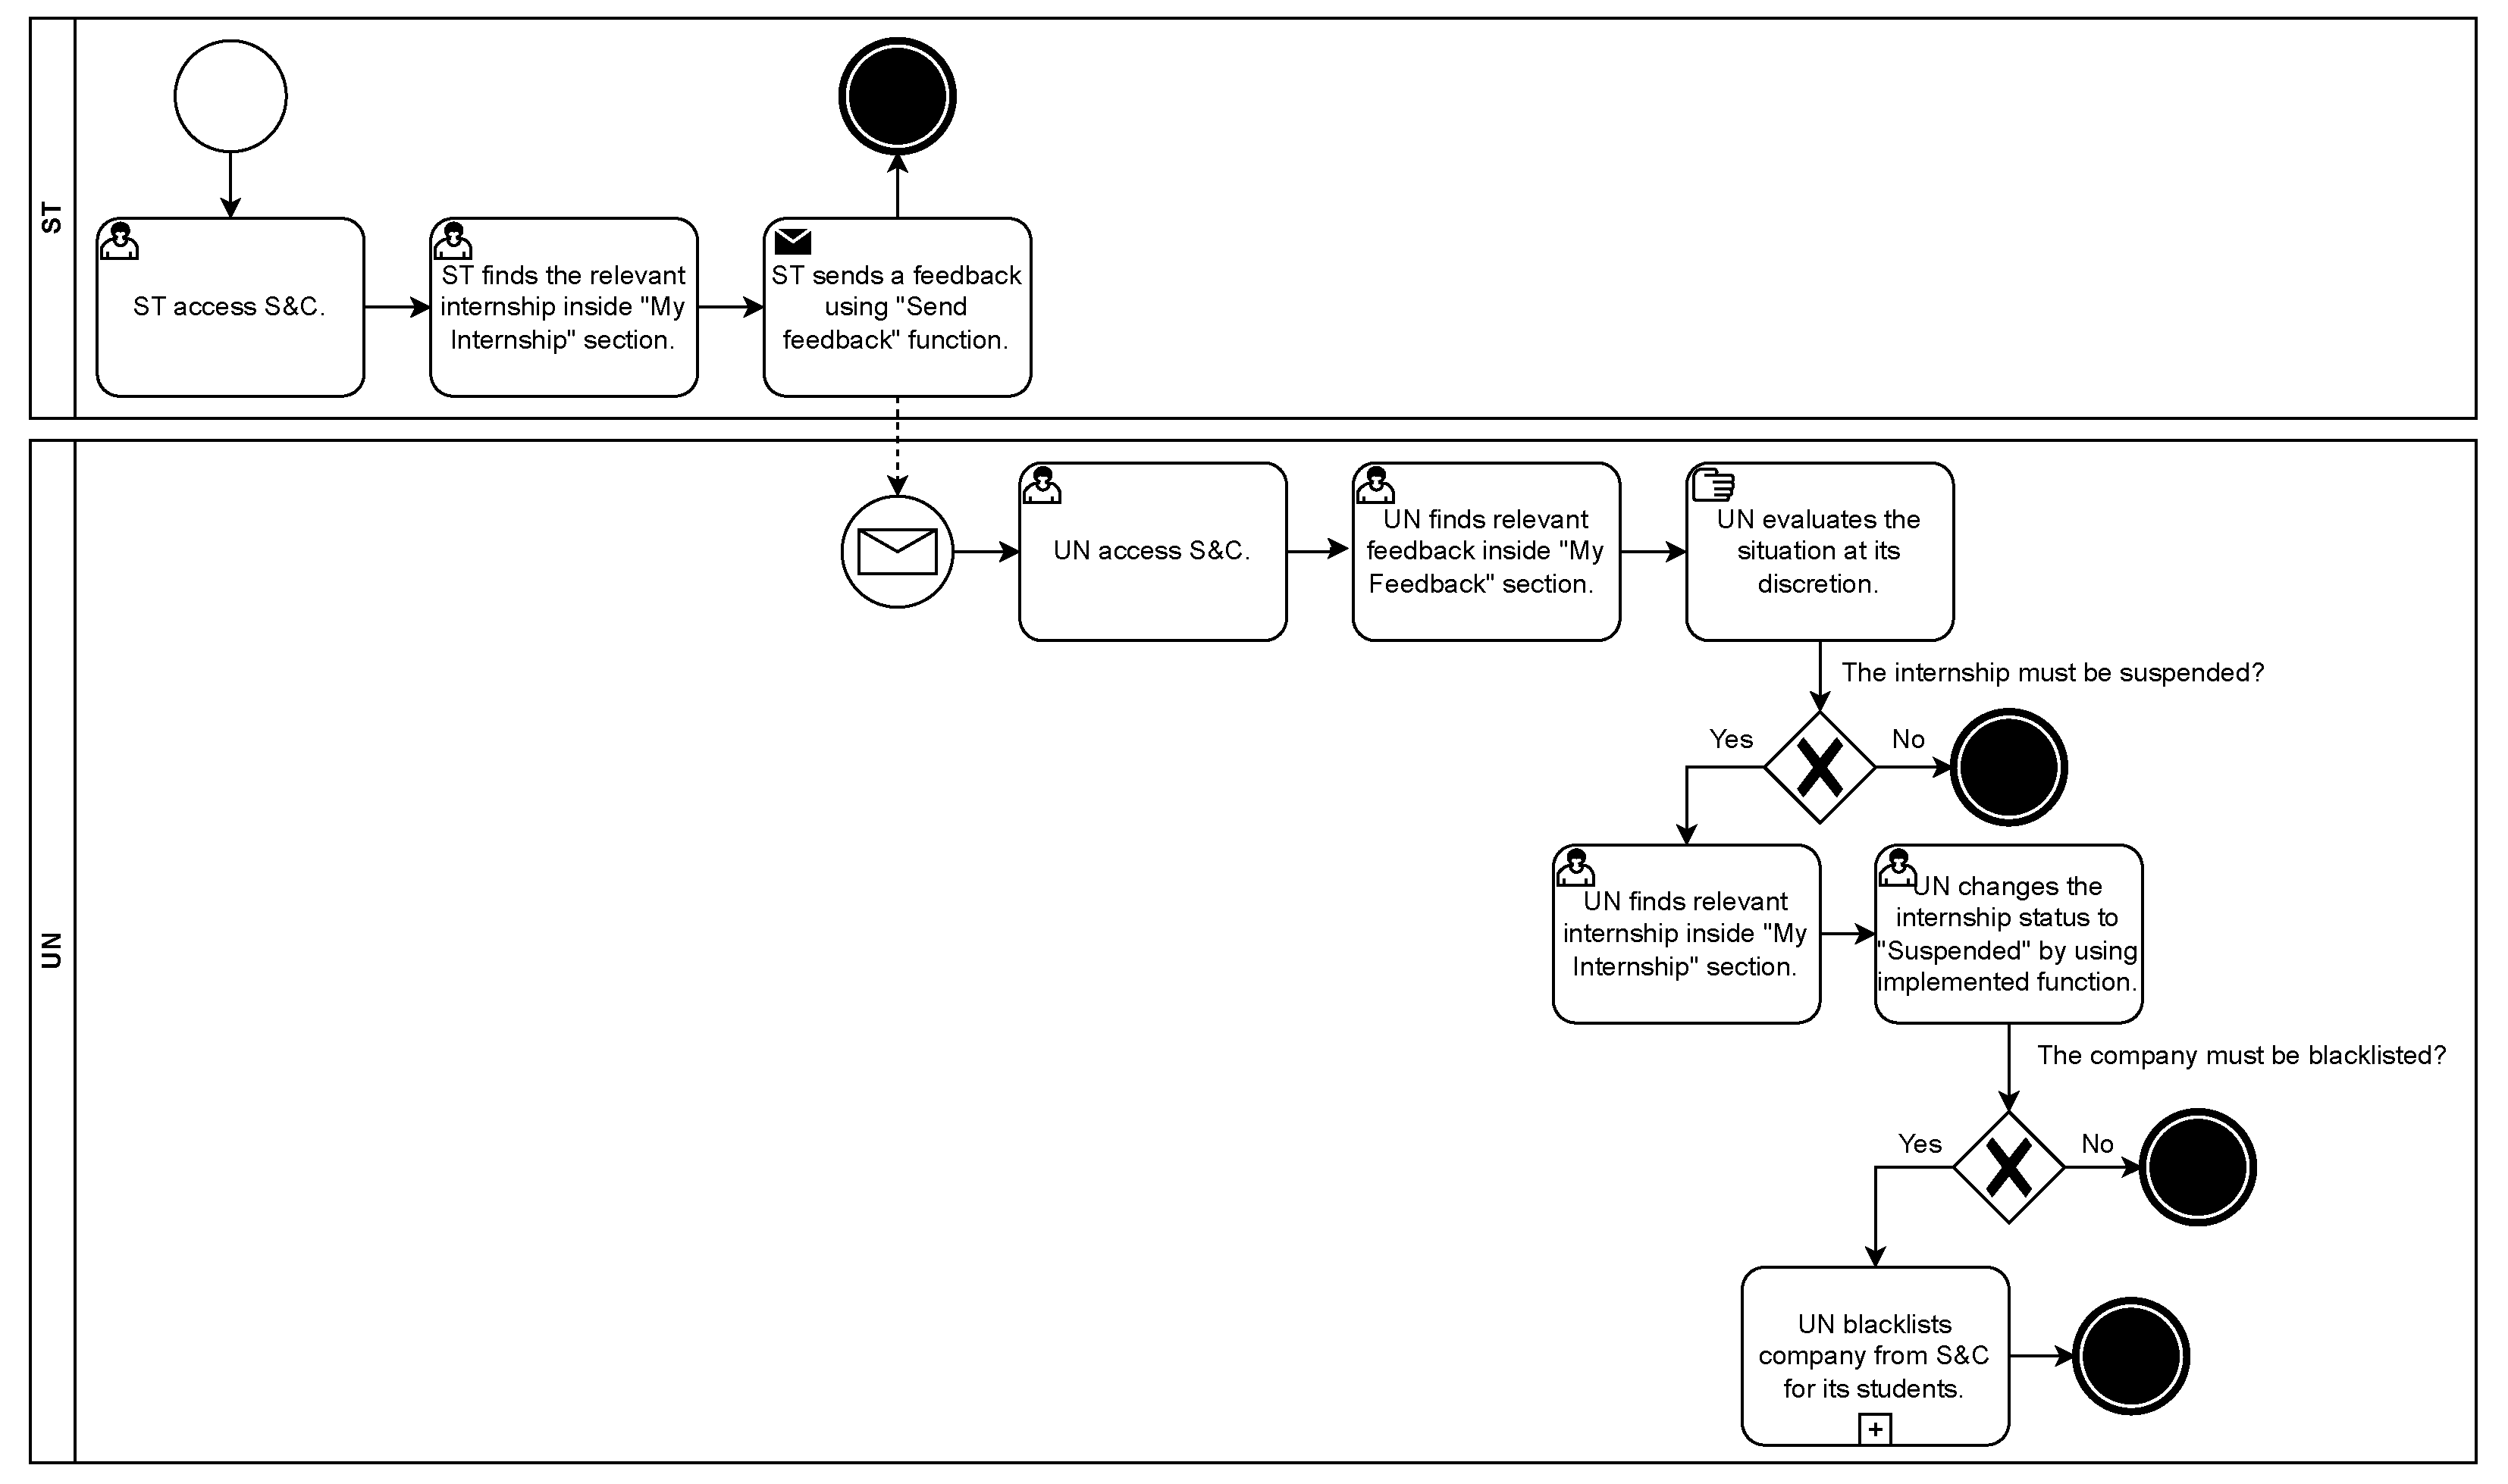
\includegraphics[width=1.0\textwidth]{Images/BPMN_15.pdf}
                  \caption{UN Complaint Handling Diagram - Product Function}
                  \label{fig:un_complaint_handling_diagram}
            \end{figure}

            \pagebreak

            % F. 16
      \item \textbf{Blacklisting}: If the university deems a company untrustworthy or has been subject to multiple
            complaints, it can blacklist it. This ensures that students at such university can’t see the company and
            vice versa, the company can’t see the university students.

            \begin{figure}[H]
                  \centering
                  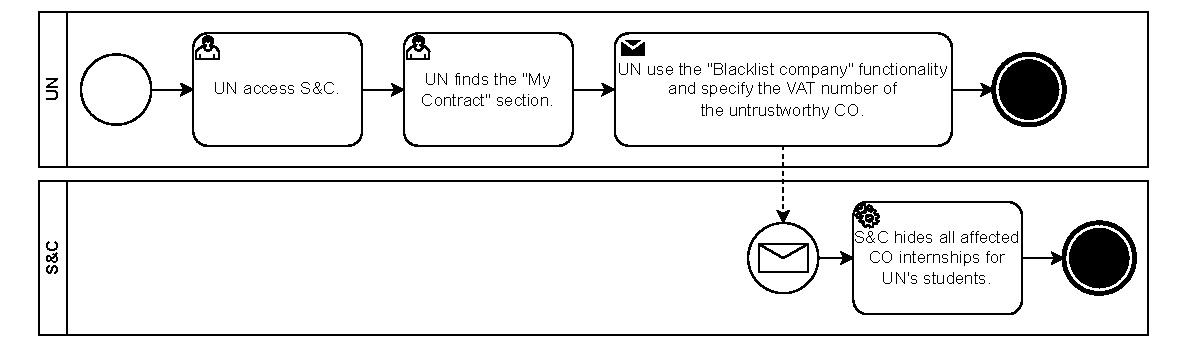
\includegraphics[width=1.0\textwidth]{Images/BPMN_16.pdf}
                  \caption{UN Blacklisting Diagram - Product Function}
                  \label{fig:un_blacklisting_diagram}
            \end{figure}

\end{itemize}

\section{User Characteristics}
\label{sec:user_characteristics}%

\par The system is designed to be used by three main actors: students, companies, and universities.

\begin{enumerate}
      \item \textbf{Students (STs)}: are verified users who access S\&C through their university credentials to find and
            apply for internships.
            \begin{enumerate}
                  \item They manage their profiles, upload CVs, and participate in company selection processes through
                        questionnaires.
                  \item The platform helps them by suggesting CV improvements and recommending relevant opportunities,
                        while also allowing them to provide feedback on their internship experiences.
            \end{enumerate}
      \item \textbf{Companies (COs)}: join S\&C through formal contracts and use the platform to post internship
            opportunities and recruit students.
            \begin{enumerate}
                  \item They maintain a corporate presence on the platform by creating detailed company profiles that
                        showcase their organization to potential interns.
                  \item They create detailed job listings, evaluate candidates through customized questionnaires, and
                        access anonymized student profiles that match their requirements (and can invite them to apply to
                        their job posting).
                  \item The platform allows them to manage the entire recruitment process, from selection to internship
                        completion, and can provide performance feedback if needed.
            \end{enumerate}
      \item \textbf{Universities (UNs)}: act as overseers of the platform, protecting their students' interests while
            monitoring internship activities.
            \begin{enumerate}
                  \item They have the authority to handle complaints, suspend internships, and blacklist problematic
                        companies.
                  \item Through their integration with S\&C, they can track their students' professional experiences and
                        provide secure authentication for student access by leveraging their existing infrastructure.
            \end{enumerate}
\end{enumerate}

\section{Assumptions, Dependencies and Constraints}
\label{sec:assumptions_dependencies_and_constraints}%

\subsection{Assumptions}
\label{sub:assumptions}%

\begin{longtable}{|l|p{0.9\textwidth}|}
      \hline
      \textbf{Assumption} & \textbf{Description}                                                                   \\
      \hline
      A01                 & Universities designate an individual to manage interactions with the website.          \\
      \hline
      A02                 & Companies have a designated HR representative to manage interactions with the website. \\
      \hline
      A03                 & Companies create internship advertisements based on positions that need to be filled.  \\
      \hline
      A04                 & Students create their CVs using standard templates to facilitate analysis.             \\
      \hline

      \caption{Domain Assumptions Table}
      \label{tab:domain_assumptions}
\end{longtable}

\subsection{Dependencies}
\label{sub:dependencies}%

\begin{longtable}{|l|p{0.9\textwidth}|}
      \hline
      \textbf{Dependency} & \textbf{Description}                                                          \\
      \hline
      D01                 & The website requires the University's Single Sign-On (SSO) for secure access. \\
      \hline
      D02                 & S\&C needs to communicate correctly with the emailing system.                 \\
      \hline

      \caption{Domain Dependencies Table}
      \label{tab:domain_dependencies}
\end{longtable}

\pagebreak

\subsection{Constraints}
\label{sub:constraints}%

\begin{longtable}{|l|p{0.9\textwidth}|}
      \hline
      \textbf{Constraint} & \textbf{Description}                                            \\
      \hline
      C01                 & All users must have the adequate devices to access the website. \\
      \hline

      \caption{Domain Constraints Table}
      \label{tab:domain_constraints}
\end{longtable}


\chapter{Specific Requirements}
\label{chap:specific-requirements}%

\par This chapter provides detailed specifications for the requirements previously mentioned that may require
additional clarification for the development team's implementation.

\section{External Interface Requirements}
\label{sec:external-interface-requirements}%

\subsection{User Interfaces}
\label{subsec:user-interfaces}%

\par The user interface of S\&C is implemented as a web-based application, making it accessible through standard web
browsers. No specialized software installation is required - users only need a web browser and an internet connection
to access all platform features.

\subsection{Hardware Interfaces}
\label{subsec:hardware-interfaces}%

\par S\&C – being a web application – will be available on all devices, connected to the internet, capable of running a
modern browser. Users can use S\&C on laptops, desktops, smartphones, tablets, ...

\subsection{Software Interfaces}
\label{subsec:software-interfaces}%

\par The system will primarily function as a standalone application. The only external dependency is the SSO portals of
the various UN organizations that have requested enrollment in S\&C, which will provide access to UN personnel and STs.

\subsection{Communication Interfaces}
\label{subsec:communication-interfaces}%

\par The system primarily relies on HTTPS for secure communication. This includes communication between users and the
frontend, as well as between the frontend and backend, and between the backend and the various SSO portals.

\par The SMTP protocol is also used to send notifications to the user's email address when necessary.

\section{Functional Requirements}
\label{sec:functional-requirements}%

\subsection{Requirements List}
\label{subsec:requirements-list}%

% Define a new counter to add an unique ID to each requirement.
\newcounter{requirementCounter}
\setcounter{requirementCounter}{0}
% Define a new command to increment the counter and return the ID (R01, R02, ...).
\newcommand{\nextRequirementID}{
    \stepcounter{requirementCounter}R\ifnum\value{requirementCounter}<10 0\fi\arabic{requirementCounter}
}

\begin{longtable}{|l|p{0.9\textwidth}|}
    \hline
    \textbf{ID}        & \textbf{Requirement}                                                                                              \\
    \hline \hline
    \nextRequirementID & S\&C integrates with UN single sign-on (SSO) systems for authentication.                                          \\
    \hline
    \nextRequirementID & S\&C enables authorized internal staff to register users as UN representatives.                                   \\
    \hline
    \nextRequirementID & S\&C enables authorized internal staff to create login credentials for CO representatives.                        \\
    \hline
    \nextRequirementID & S\&C supports new ST registration through their UN's SSO system.                                                  \\
    \hline
    \nextRequirementID & S\&C enables existing ST users to log in through their UN's SSO system.                                           \\
    \hline
    \nextRequirementID & S\&C enables registered CO representatives to log in using their assigned credentials.                            \\
    \hline
    \nextRequirementID & S\&C enables registered UN representatives to log in through their UN's SSO system.                               \\
    \hline
    \nextRequirementID & S\&C enables STs to upload and store their CVs on the platform.                                                   \\
    \hline
    \nextRequirementID & S\&C provides automated CV feedback and improvement suggestions to STs.                                           \\
    \hline
    \nextRequirementID & S\&C allows STs to browse all publicly available internship opportunities.                                        \\
    \hline
    \nextRequirementID & S\&C provides filtering capabilities (by keyword, company, etc.) for internship searches.                         \\
    \hline
    \nextRequirementID & S\&C implements a recommendation system to suggest relevant internships to STs.                                   \\
    \hline
    \nextRequirementID & S\&C sends email notifications to STs about recommended internships.                                              \\
    \hline
    \nextRequirementID & S\&C displays comprehensive internship information for each listing.                                              \\
    \hline
    \nextRequirementID & S\&C integrates CO profiles within internship listing details.                                                    \\
    \hline
    \nextRequirementID & S\&C enables STs to submit internship applications before specified deadlines.                                    \\
    \hline
    \nextRequirementID & S\&C notifies STs when COs request questionnaire completion.                                                      \\
    \hline
    \nextRequirementID & S\&C allows STs to complete CO-specific questionnaires when requested.                                            \\
    \hline
    \nextRequirementID & S\&C provides a system for STs to submit concerns or complaints during their internship.                          \\
    \hline
    \nextRequirementID & S\&C notifies STs of any resolution or changes resulting from their submitted complaints.                         \\
    \hline
    \nextRequirementID & S\&C facilitates post-internship feedback collection from STs.                                                    \\
    \hline
    \nextRequirementID & S\&C enables COs to create and publish internship listings.                                                       \\
    \hline
    \nextRequirementID & S\&C allows COs to specify application deadlines for internship positions.                                        \\
    \hline
    \nextRequirementID & S\&C provides automated suggestions to improve internship listing content.                                        \\
    \hline
    \nextRequirementID & S\&C displays ST's anonymized CVs to be seen by COs.                                                              \\
    \hline
    \nextRequirementID & S\&C enables COs to create evaluation questionnaires for applicants.                                              \\
    \hline
    \nextRequirementID & S\&C allows COs to distribute questionnaires to selected candidates.                                              \\
    \hline
    \nextRequirementID & S\&C provides COs access to completed questionnaire responses.                                                    \\
    \hline
    \nextRequirementID & S\&C enables COs to update the status of their internship listings.                                               \\
    \hline
    \nextRequirementID & S\&C provides a system for COs to submit concerns or complaints during internships.                               \\
    \hline
    \nextRequirementID & S\&C notifies COs of any changes regarding their internship statues.                                              \\
    \hline
    \nextRequirementID & S\&C facilitates post-internship feedback collection from COs.                                                    \\
    \hline
    \nextRequirementID & S\&C enables UNs to monitor the status of all its STs internships.                                                \\
    \hline
    \nextRequirementID & S\&C provides UNs access to feedback of their STs internship from both COs and STs, including submitted details.  \\
    \hline
    \nextRequirementID & S\&C notifies UNs when new feedback is submitted by any party.                                                    \\
    \hline
    \nextRequirementID & S\&C allows UNs to block COs that violate platform guidelines or trust.                                           \\
    \hline
    \nextRequirementID & S\&C enables UNs to modify the status of internship positions.                                                    \\
    \hline
    \nextRequirementID & S\&C notifies STs of any changes to their internship status.                                                      \\
    \hline
    \nextRequirementID & S\&C allows COs to see the full CV of STs once they have been evaluated by the questionnaires.                    \\
    \hline
    \nextRequirementID & S\&C allows COs to edit their company profile to be seen by STs.                                                  \\
    \hline
    \nextRequirementID & S\&C computes for each internship a pool of recommended candidates.                                               \\
    \hline
    \nextRequirementID & S\&C notifies COs when new recommended candidates are available. And they have not yet applied to the internship. \\
    \hline
    \nextRequirementID & S\&C allows COs to asks - to the recommended candidates - to apply to the internship.                             \\
    \hline
    \caption{Requirements Table}
    \label{tab:requirements-table}
\end{longtable}

\subsection{Use Case Diagrams}
\label{subsec:use-case-diagrams}

\begin{figure}[H]
    \centering
    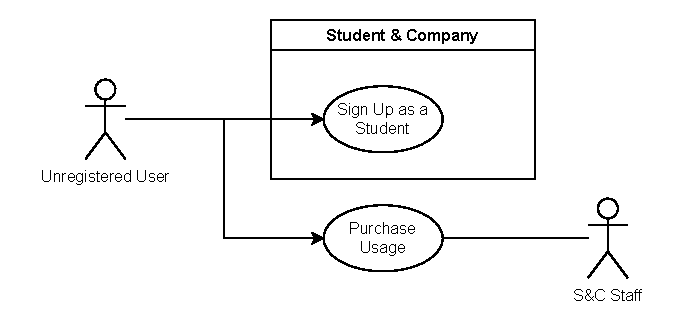
\includegraphics[width=1.0\textwidth]{Images/UC_Unregistered_User.pdf}
    \caption{Use Case Diagram for Unregistered Users}
    \label{fig:use-case-diagram-unregistered-user}
\end{figure}

\begin{figure}[H]
    \centering
    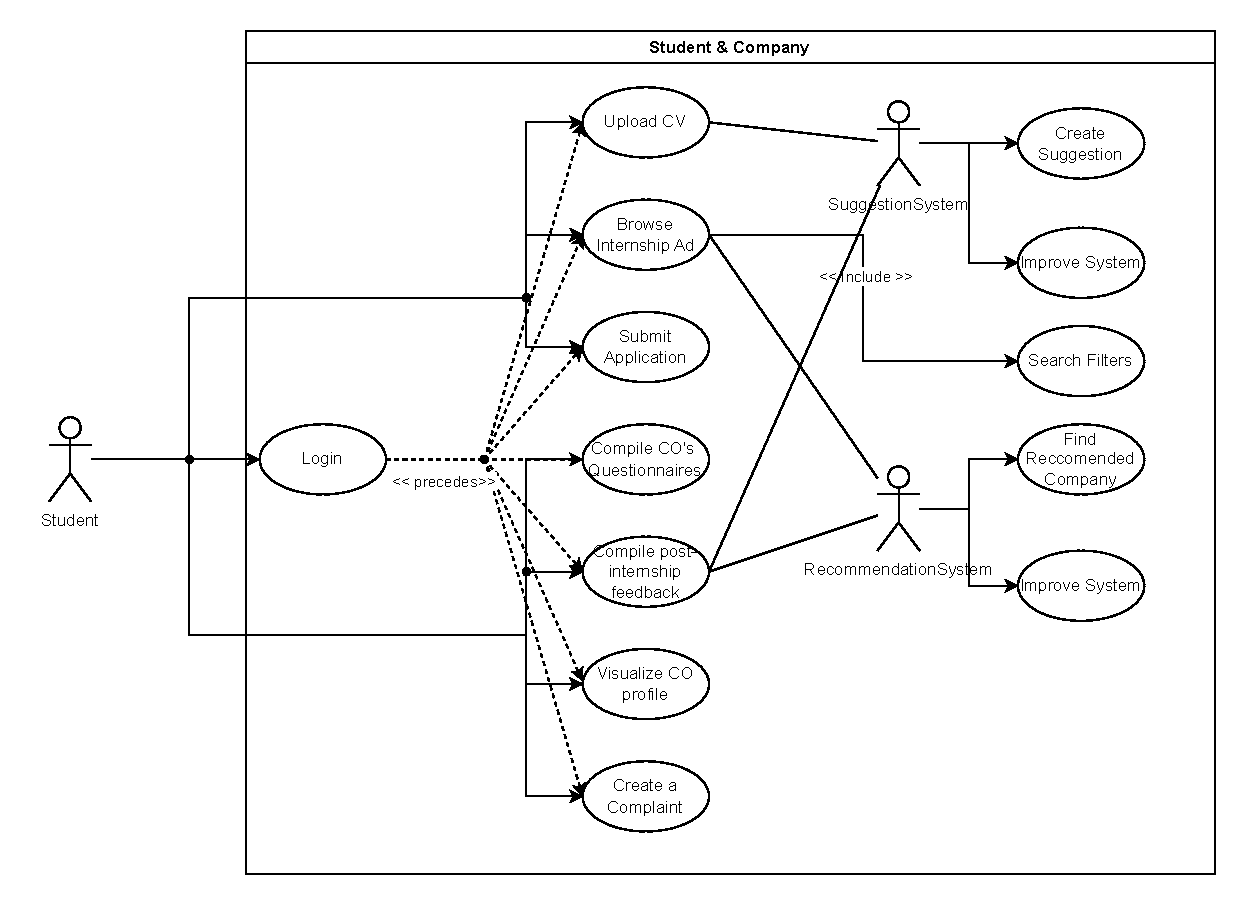
\includegraphics[width=1.0\textwidth]{Images/UC_Student.pdf}
    \caption{Use Case Diagram for Students}
    \label{fig:use-case-diagram-students}
\end{figure}

\begin{figure}[H]
    \centering
    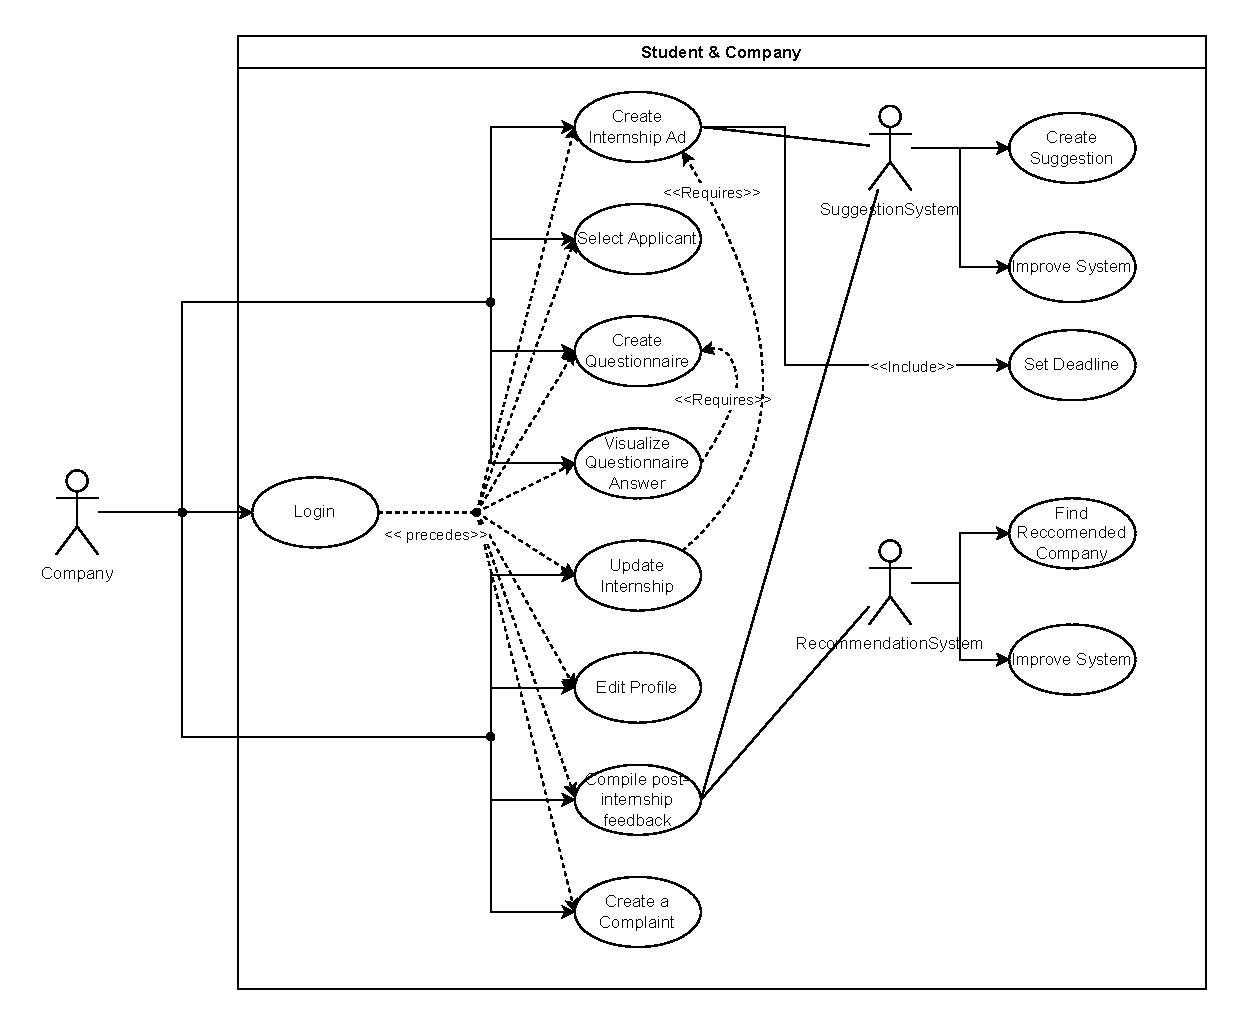
\includegraphics[width=1.0\textwidth]{Images/UC_Company.pdf}
    \caption{Use Case Diagram for Companies}
    \label{fig:use-case-diagram-companies}
\end{figure}

\begin{figure}[H]
    \centering
    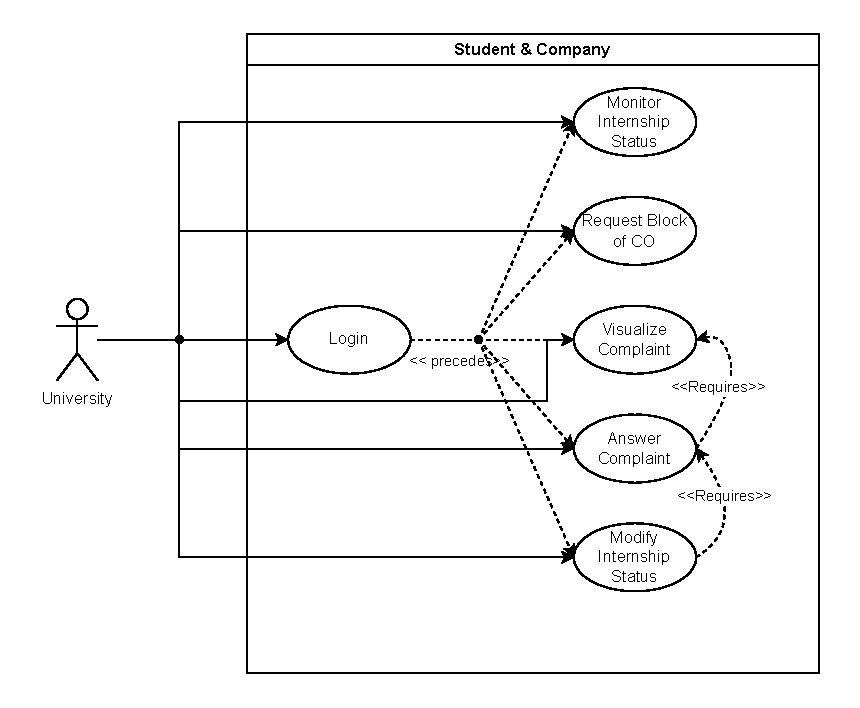
\includegraphics[width=1.0\textwidth]{Images/UC_University.pdf}
    \caption{Use Case Diagram for Universities}
    \label{fig:use-case-diagram-universities}
\end{figure}

\subsection{Use Cases}
\label{subsec:use-cases}

\par In this section, a detailed description of the main use cases of the system is presented.
Each use case is described by a table containing the actors, entry conditions, flow of events, exit conditions, and exceptions.
The use case diagram shows the messages exchanged between the actors and the system and the functions called by them.

% 01

\subsubsection{UC01: Student login}
\label{subsubsec:student-login}
\begin{center}
    \begin{longtable}{|l|p{0.75\linewidth}|}
        \hline
        \textbf{Actors:}           & ST                                                                            \\
        \hline
        \textbf{Entry Conditions:} & The student university is subscribed to S\&C services.                        \\
        \hline
        \textbf{Flow of Events:}   & \begin{enumerate}
                                         \item ST searches for the URL of the S\&C login page.
                                         \item S\&C sends the login web page to the ST.
                                         \item ST inserts the username and password used to log in to their university.
                                         \item S\&C receives the credentials.
                                         \item S\&C forwards the credentials to the university database.
                                         \item The university database validates the credentials.
                                         \item S\&C returns a session token to the ST.
                                     \end{enumerate} \\
        \hline
        \textbf{Exit condition:}   & ST has logged in successfully to S\&C.                                        \\
        \hline
        \textbf{Exceptions:}       & \begin{enumerate}
                                         \item The credentials are wrong.
                                         \item The ST was blocked by the S\&C staff.
                                         \item S\&C generated an internal error.
                                     \end{enumerate}                                    \\
        \hline
    \end{longtable}
\end{center}

\begin{figure}[H]
    \centering
    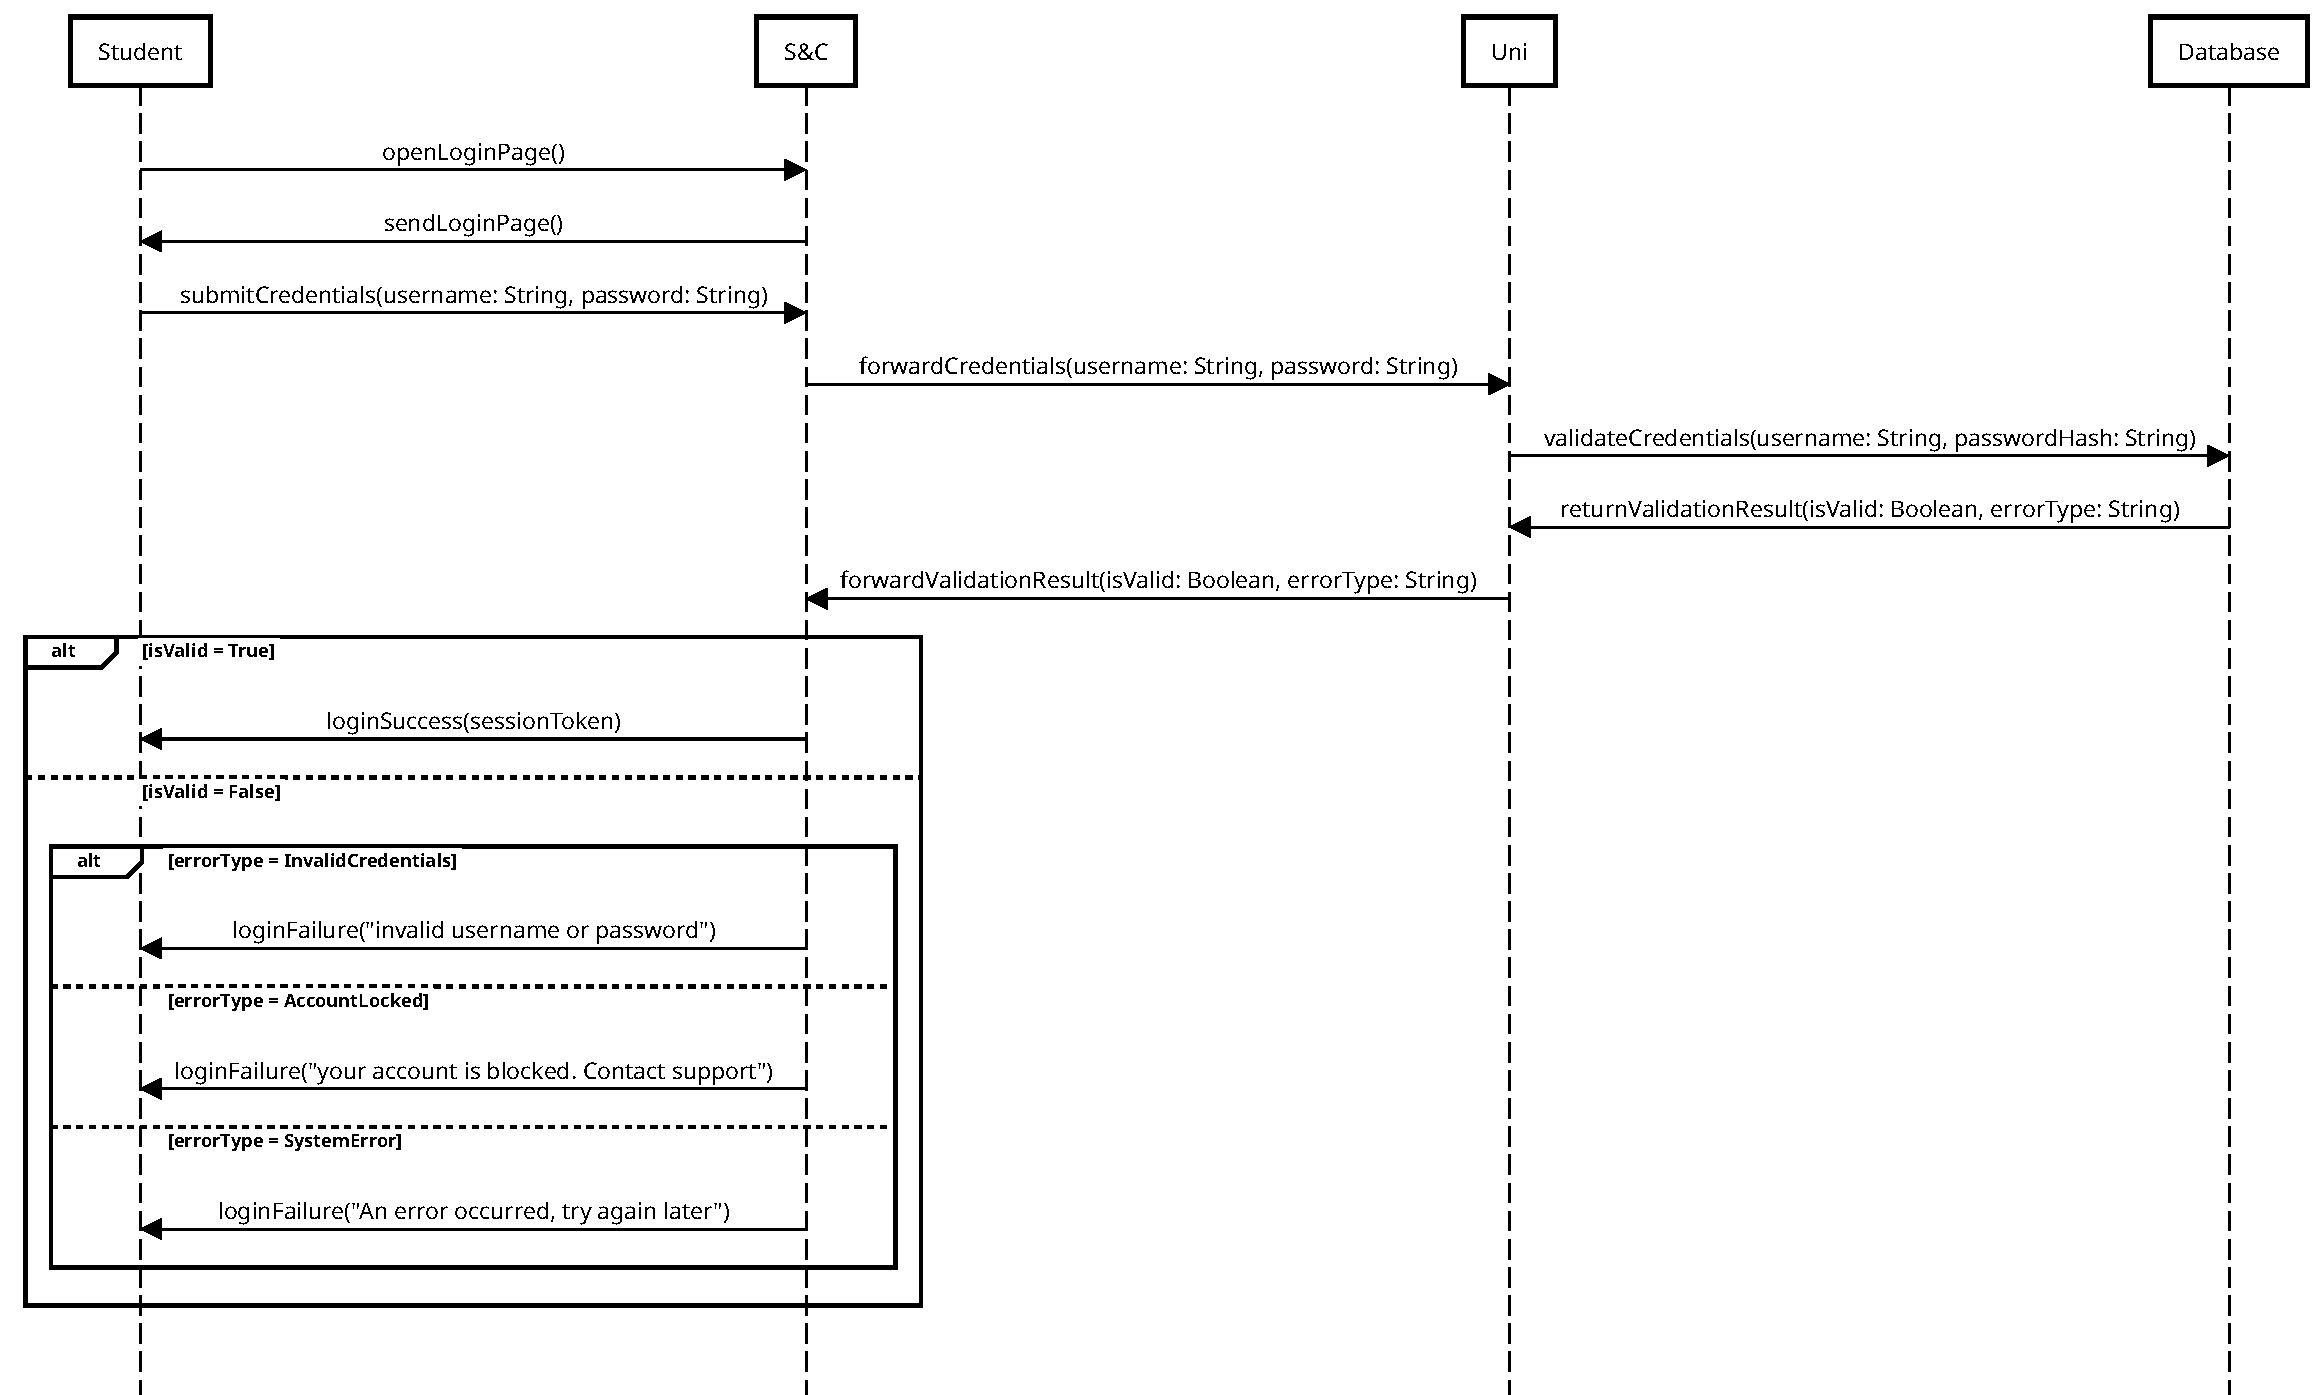
\includegraphics[width=1.0\textwidth]{Images/UC_1.pdf}
    \caption{Student Login - Use Case Diagram}
    \label{fig:use-case-diagram-1}
\end{figure}

% 2

\subsubsection{UC02: Student uploads its CV and receives suggestions}
\label{subsubsec:studend-upload-CV}
\begin{center}
    \begin{longtable}{|l|p{0.75\linewidth}|}
        \hline
        \textbf{Actors:}           & ST                                                                                                    \\
        \hline
        \textbf{Entry Conditions:} & ST is correctly logged in to S\&C.                                                                    \\
        \hline
        \textbf{Flow of Events:}   & \begin{enumerate}
                                         \item ST visits the "My CV" page.
                                         \item ST uploads the CV file to S\&C.
                                         \item S\&C stores the CV in the database.
                                         \item The insert/update operation on the S\&C database triggers the CV suggestion system.
                                         \item The suggestion system fetches the CV from the database and analyzes it.
                                         \item The suggestion system generates feedback and improvement suggestions and stores them.
                                         \item The ST can see the suggestions by clicking on the "Show suggestions" button on the "My CV" page.
                                     \end{enumerate} \\
        \hline
        \textbf{Exit Conditions:}  & ST has successfully uploaded the CV and received suggestions.                                         \\
        \hline
        \textbf{Exceptions:}       & The ST tries to get the suggestions before they are ready.                                            \\                                                      \\
        \hline
    \end{longtable}
\end{center}

\begin{figure}[H]
    \centering
    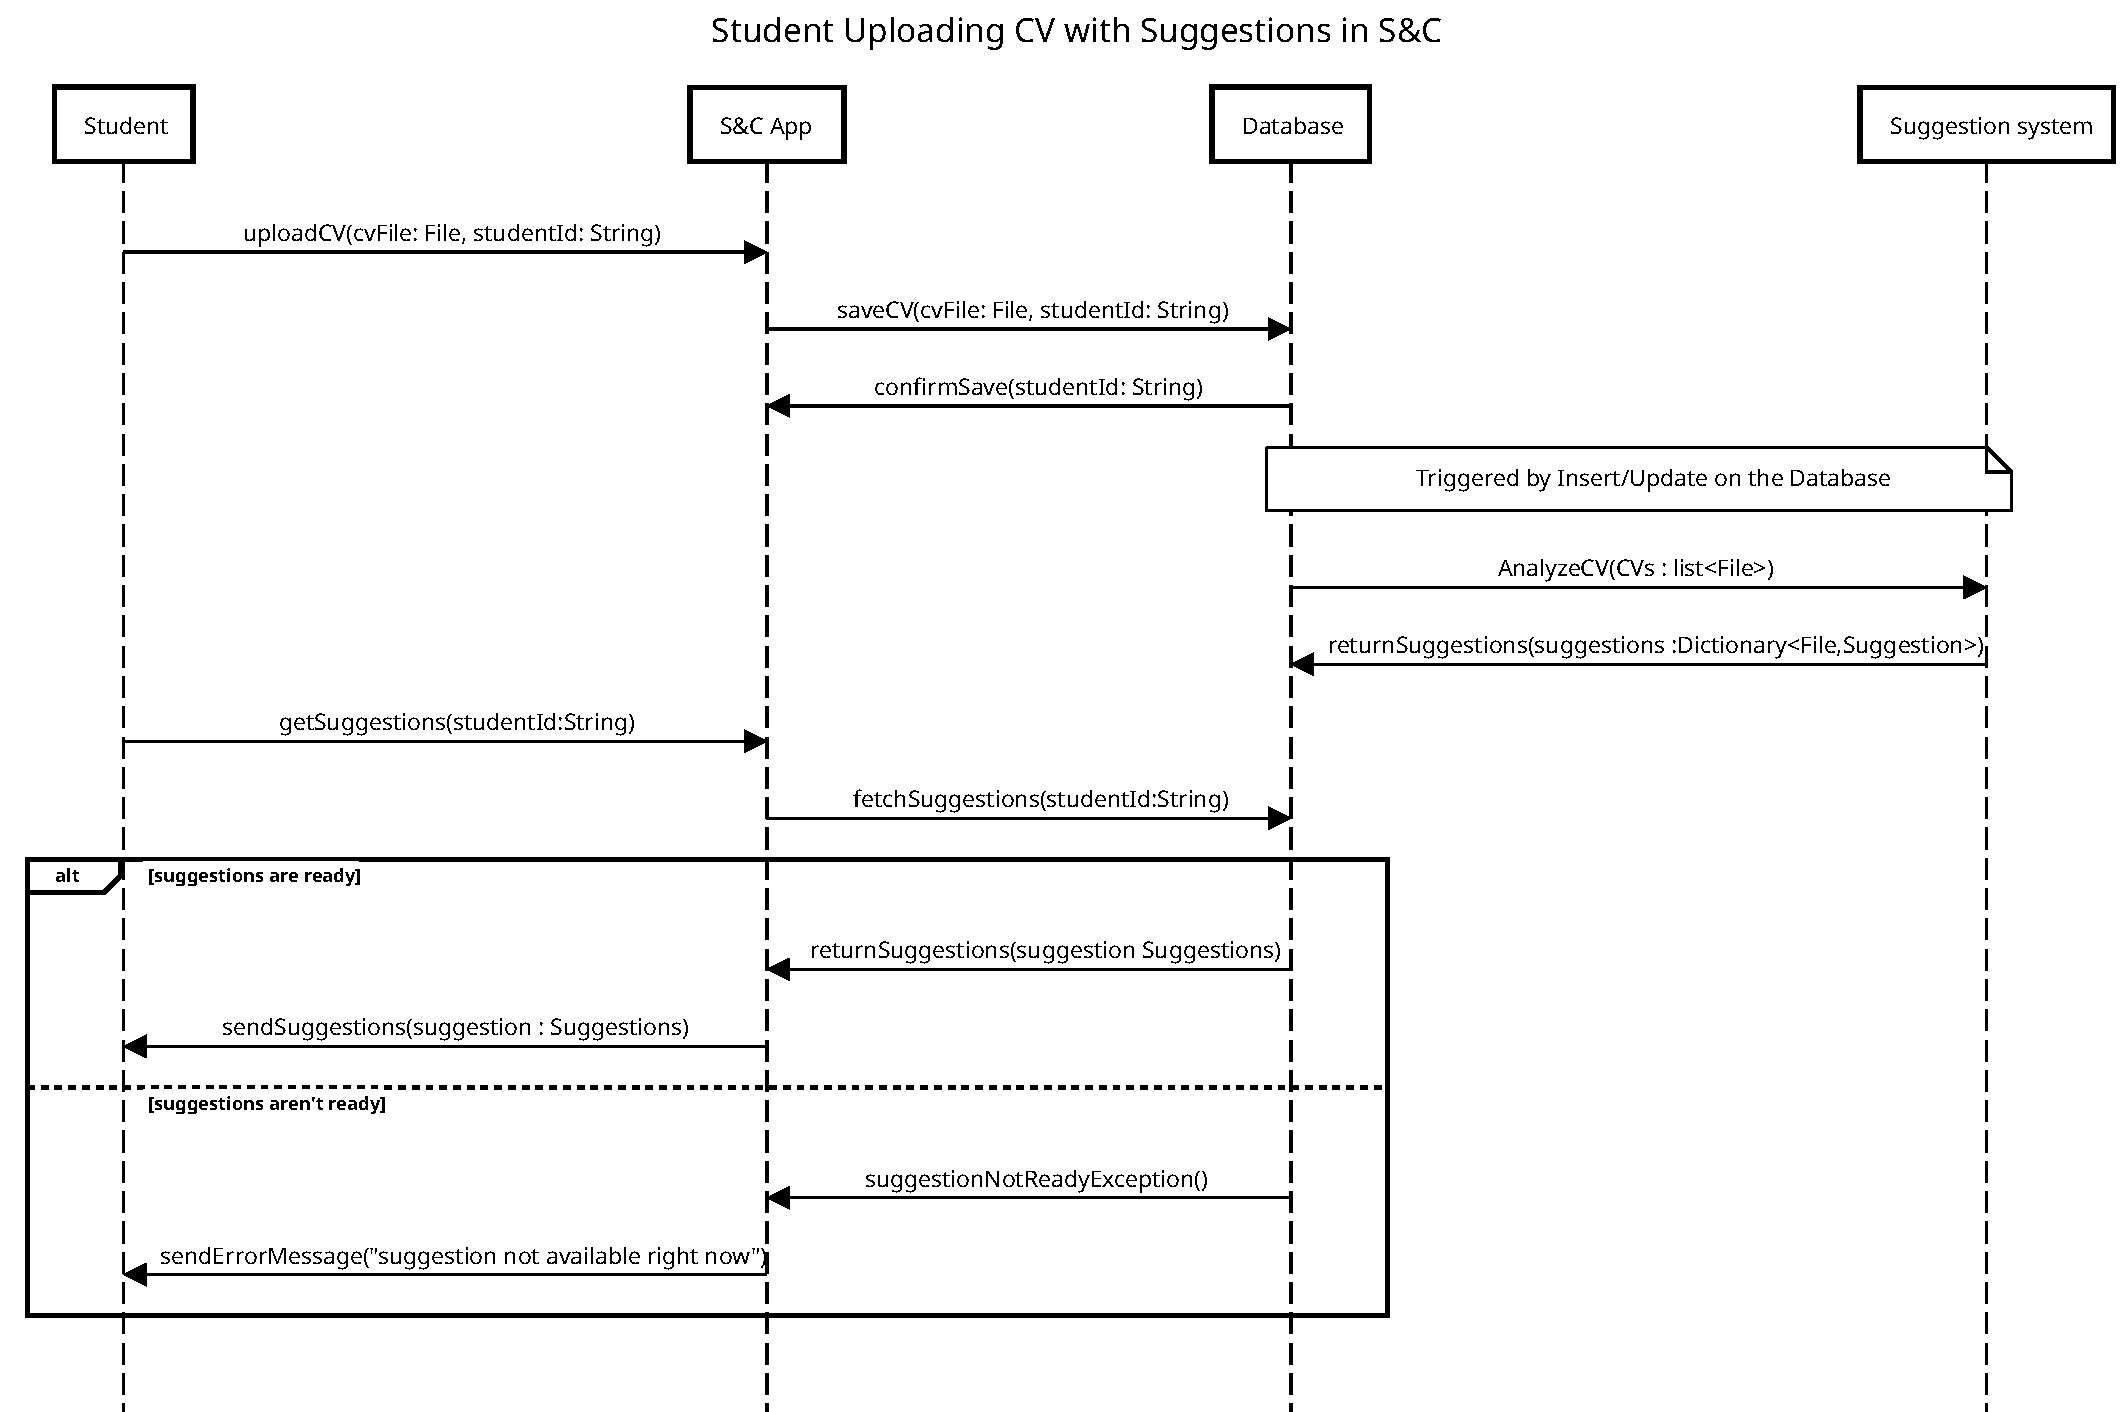
\includegraphics[width=1.0\textwidth]{Images/UC_2.pdf}
    \caption{Student Uploads its CV and Receives Suggestions - Use Case Diagram}
    \label{fig:use-case-diagram-2}
\end{figure}

% 3

\subsubsection{UC03: Student internship advertisement search}
\label{subsubsec:student-internship-advertisement-search}

\begin{center}
    \begin{longtable}{|l|p{0.75\linewidth}|}
        \hline
        \textbf{Actors:}           & ST                                                        \\
        \hline
        \textbf{Entry Conditions:} & ST is correctly logged in.                                \\
        \hline
        \textbf{Flow of Events:}   & \begin{enumerate}
                                         \item ST visits the "Internships" page.
                                         \item S\&C fetch the internships from the database.
                                         \item S\&C shows the internships to the ST.
                                         \item ST filters the internships by keyword, company, etc.
                                         \item S\&C shows the filtered internships to the ST.
                                         \item ST selects an internship to view the details.
                                         \item S\&C fetch the internship details from the database.
                                         \item S\&C shows the internship details to the ST.
                                     \end{enumerate} \\
        \hline
        \textbf{Exit Conditions:}  & ST has successfully viewed the internships.               \\
        \hline
        \textbf{Exceptions:}       & S\&C generated an internal error.                         \\
        \hline
    \end{longtable}
\end{center}

\begin{figure}[H]
    \centering
    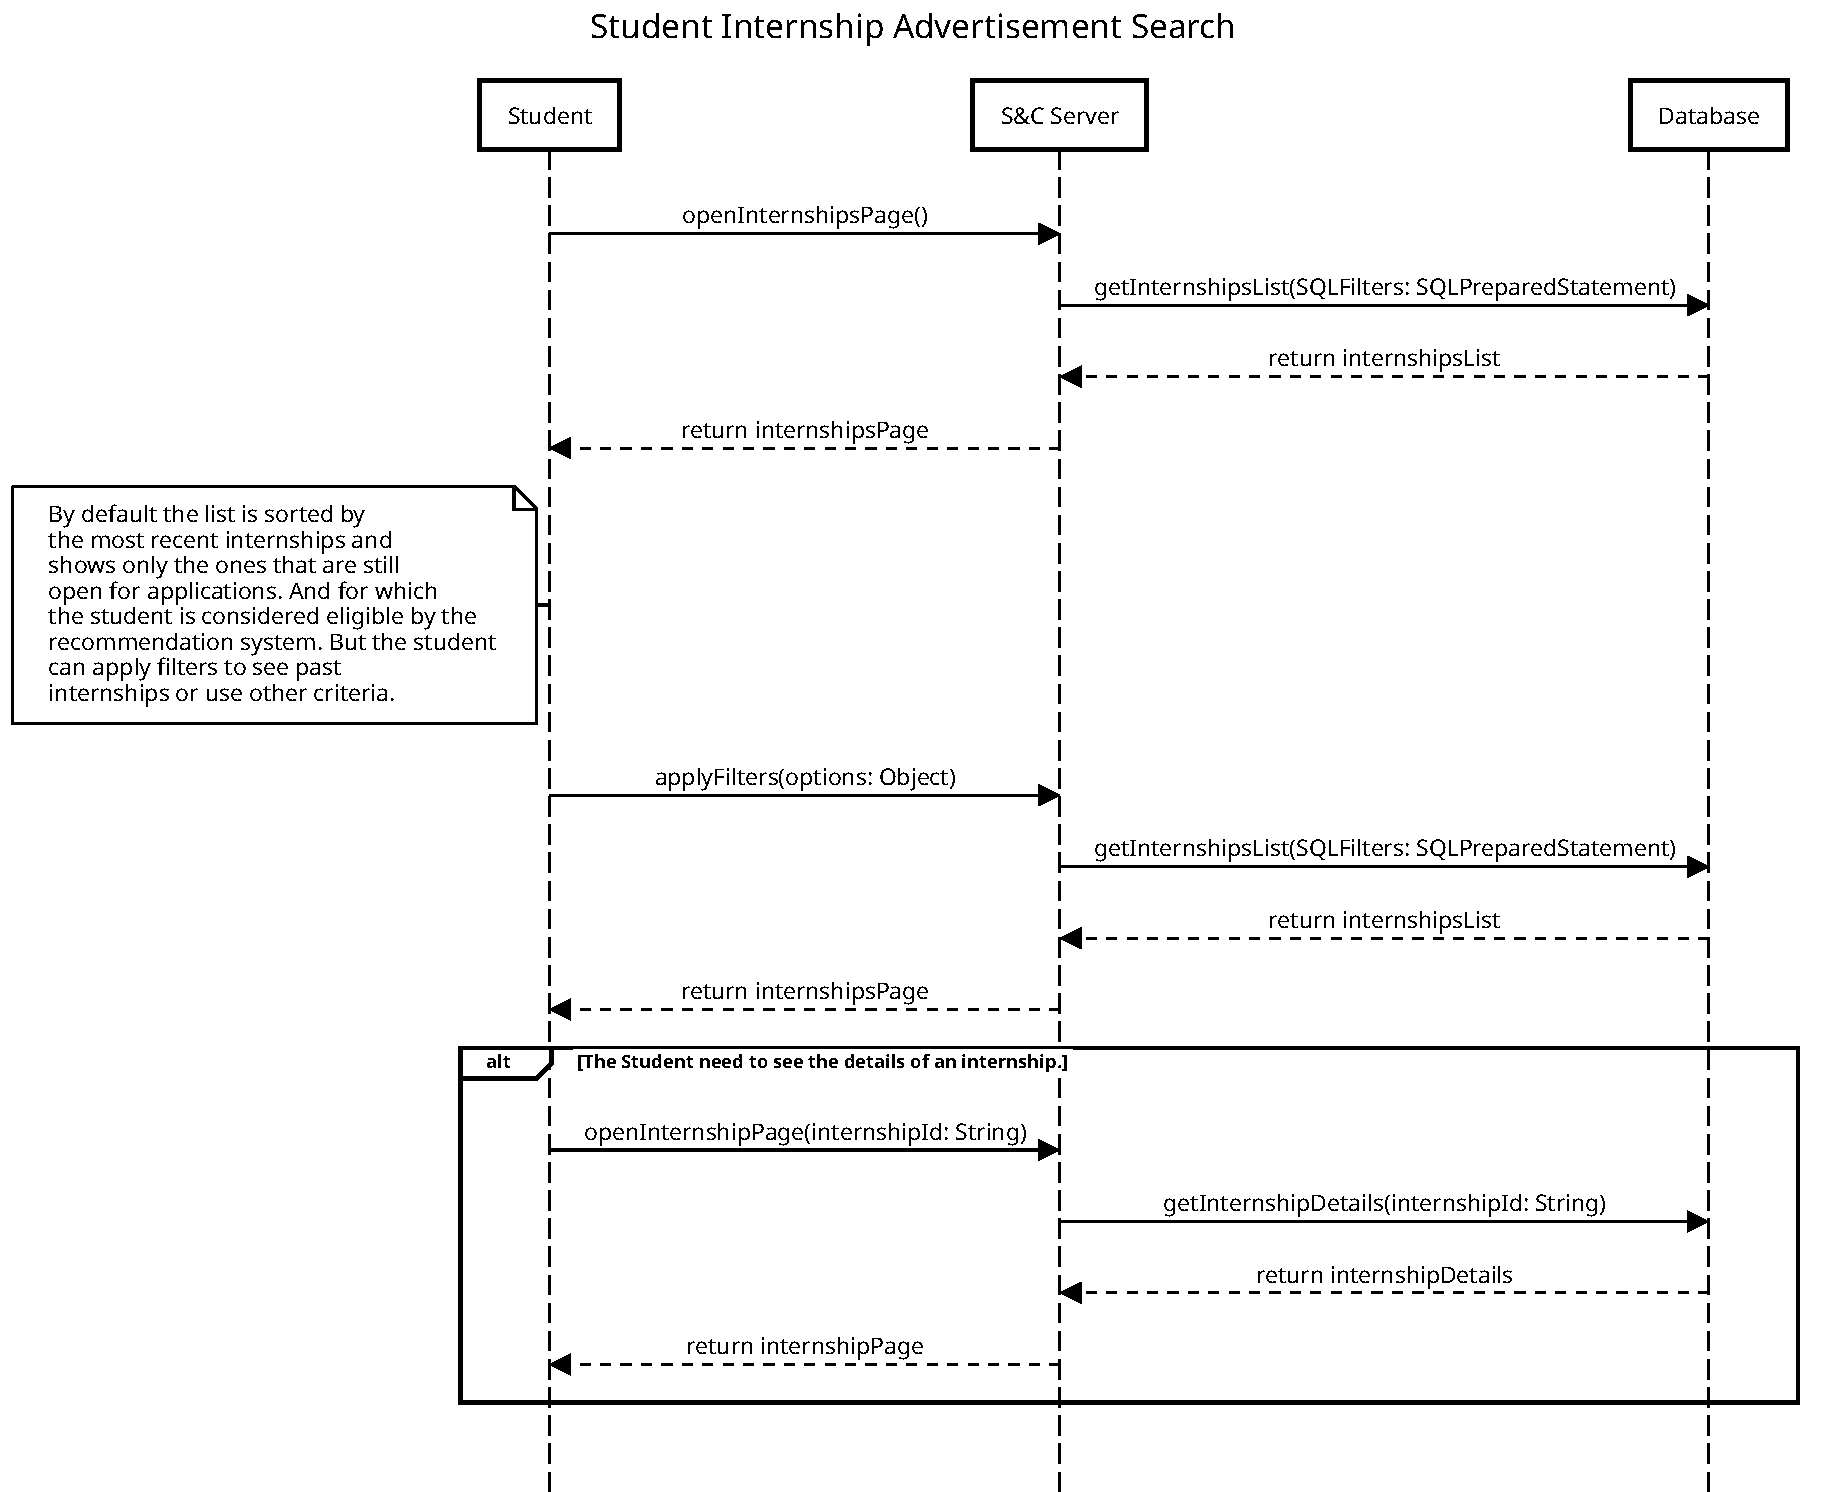
\includegraphics[width=1.0\textwidth]{Images/UC_3.pdf}
    \caption{Student Internship Advertisement Search - Use Case Diagram}
    \label{fig:use-case-diagram-3}
\end{figure}

% 4

\subsubsection{UC04: Student applies to an internship}
\label{subsubsec:student-applies-to-an-internship}

\begin{center}
    \begin{longtable}{|l|p{0.75\linewidth}|}
        \hline
        \textbf{Actors:}           & ST, CO                                                               \\
        \hline
        \textbf{Entry Conditions:} & ST is correctly logged in.                                           \\
        \hline
        \textbf{Flow of Events:}   & \begin{enumerate}
                                         \item ST visits the "Internships" page.
                                         \item S\&C fetch the internships from the database.
                                         \item S\&C shows the internships to the ST.
                                         \item ST selects an internship to view the details.
                                         \item S\&C fetch the internship details from the database.
                                         \item S\&C shows the internship details to the ST.
                                         \item ST clicks on the "Apply" button.
                                         \item S\&C stores the application in the database.
                                         \item S\&C notifies the CO that the ST has applied to the internship.
                                     \end{enumerate} \\
        \hline
        \textbf{Exit Conditions:}  & ST has successfully applied to the internship.                       \\
        \hline
        \textbf{Exceptions:}       & S\&C generated an internal error.                                    \\
        \hline
    \end{longtable}
\end{center}

\begin{figure}[H]
    \centering
    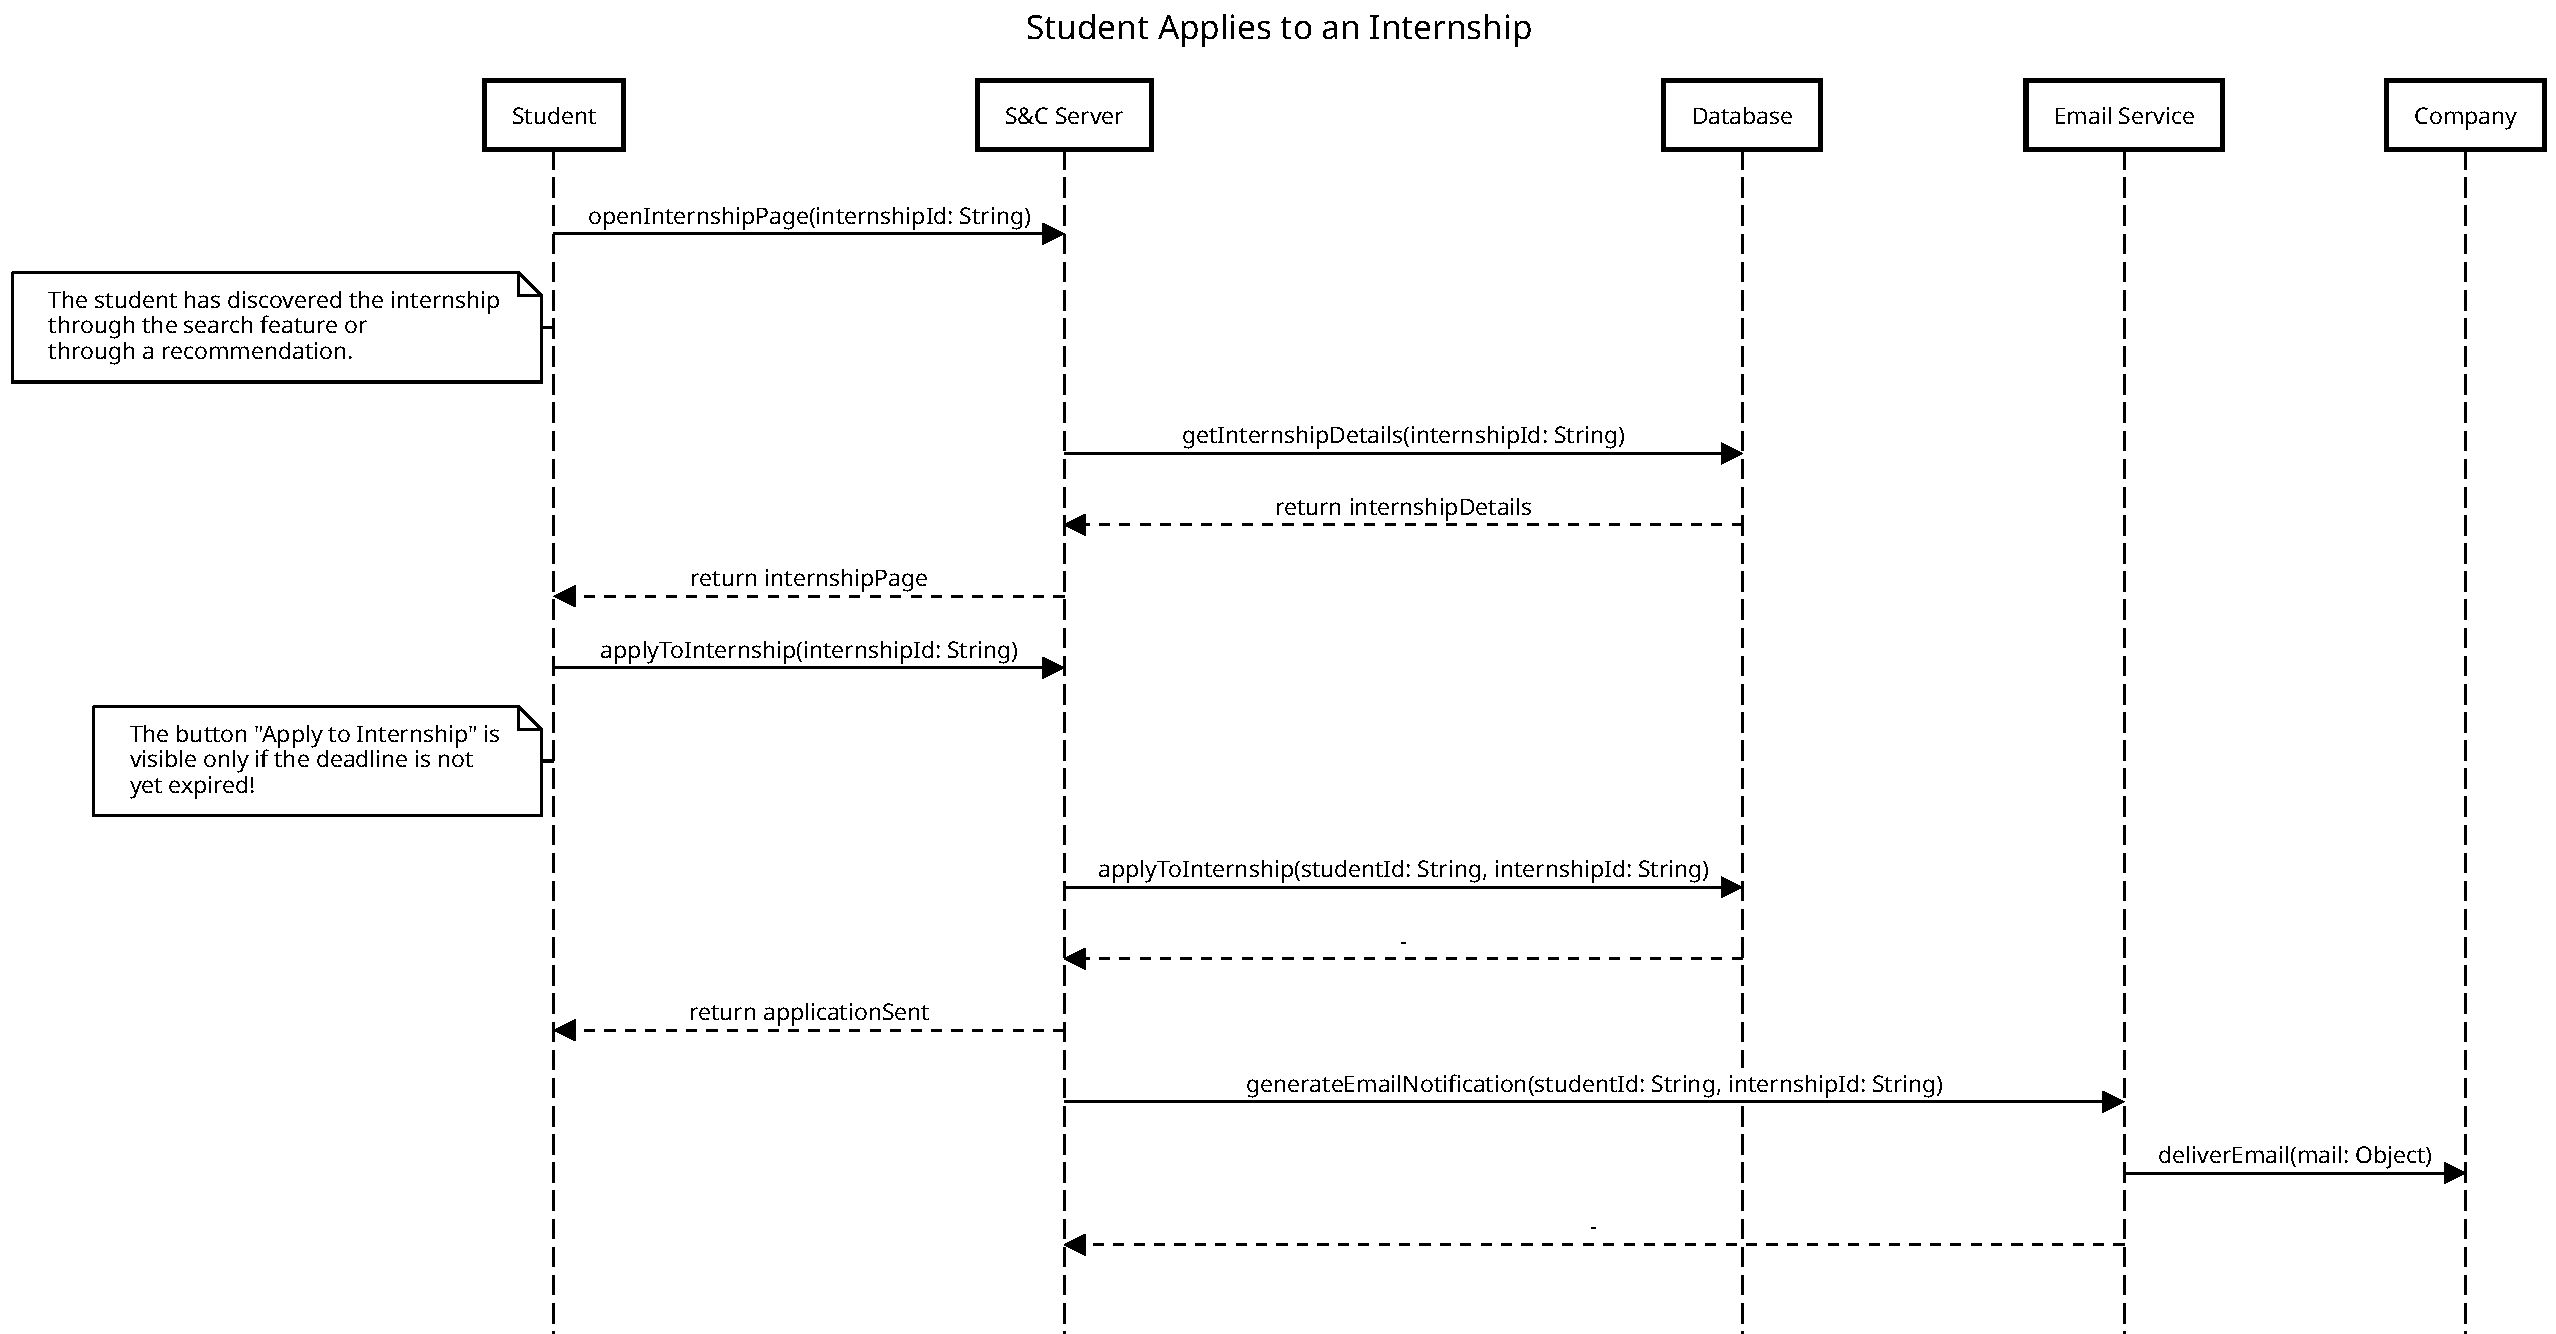
\includegraphics[width=1.0\textwidth]{Images/UC_4.pdf}
    \caption{Student Applies to an Internship - Use Case Diagram}
    \label{fig:use-case-diagram-4}
\end{figure}

% 5

\subsubsection{UC05: Student answers a company questionnaire}
\label{subsubsec:student-answers-a-company-questionnaire}

\begin{center}
    \begin{longtable}{|l|p{0.75\linewidth}|}
        \hline
        \textbf{Actors:}           & ST, CO                                                                             \\
        \hline
        \textbf{Entry Conditions:} & CO has requested ST to fill a questionnaire.                                       \\
        \hline
        \textbf{Flow of Events:}   & \begin{itemize}
                                         \item (opt. 1) ST uses the link sent by S\&C via email to access the questionnaire.
                                               \begin{enumerate}
                      \item S\&C verify if the link is valid.
                            \begin{itemize}
                                \item Link valid and not expired: the flow continues.
                                \item Link invalid or expired: ST is redirected to the questionnaire page.
                            \end{itemize}
                  \end{enumerate}
                                         \item (opt. 2) ST finds the questionnaire directly on the S\&C platform.
                                               \begin{enumerate}
                      \item ST visits the "My Internships" page.
                      \item S\&C fetch the internships from the database.
                      \item S\&C shows the internships to the ST.
                      \item ST selects an internship to view the details.
                      \item S\&C fetch the internship details from the database.
                      \item S\&C shows the internship details to the ST.
                      \item ST clicks on the "Compile the Questionnaire" button.
                      \item ST is redirected to the questionnaire page.
                  \end{enumerate}
                                         \item S\&C fetch the questionnaire from the database.
                                         \item S\&C shows the questionnaire to the ST.
                                         \item ST starts to fill the questionnaire. For each question:
                                               \begin{enumerate}
                      \item ST gives an answer.
                      \item S\&C stores the answer in the database.
                  \end{enumerate}
                                         \item ST ends its job and submits the questionnaire.
                                         \item S\&C stores that the questionnaire was submitted.
                                         \item S\&C notifies the CO that the questionnaire was successfully submitted.
                                         \item S\&C evaluates the answers and compute the final score.
                                         \item S\&C the final score is stored to be consulted by the CO later.
                                     \end{itemize} \\
        \hline
        \textbf{Exit Conditions:}  & ST has successfully filled the questionnaire.                                      \\
        \hline
        \textbf{Exceptions:}       & S\&C generated an internal error. The link is invalid or expired.                  \\
        \hline
    \end{longtable}
\end{center}

\begin{figure}[H]
    \centering
    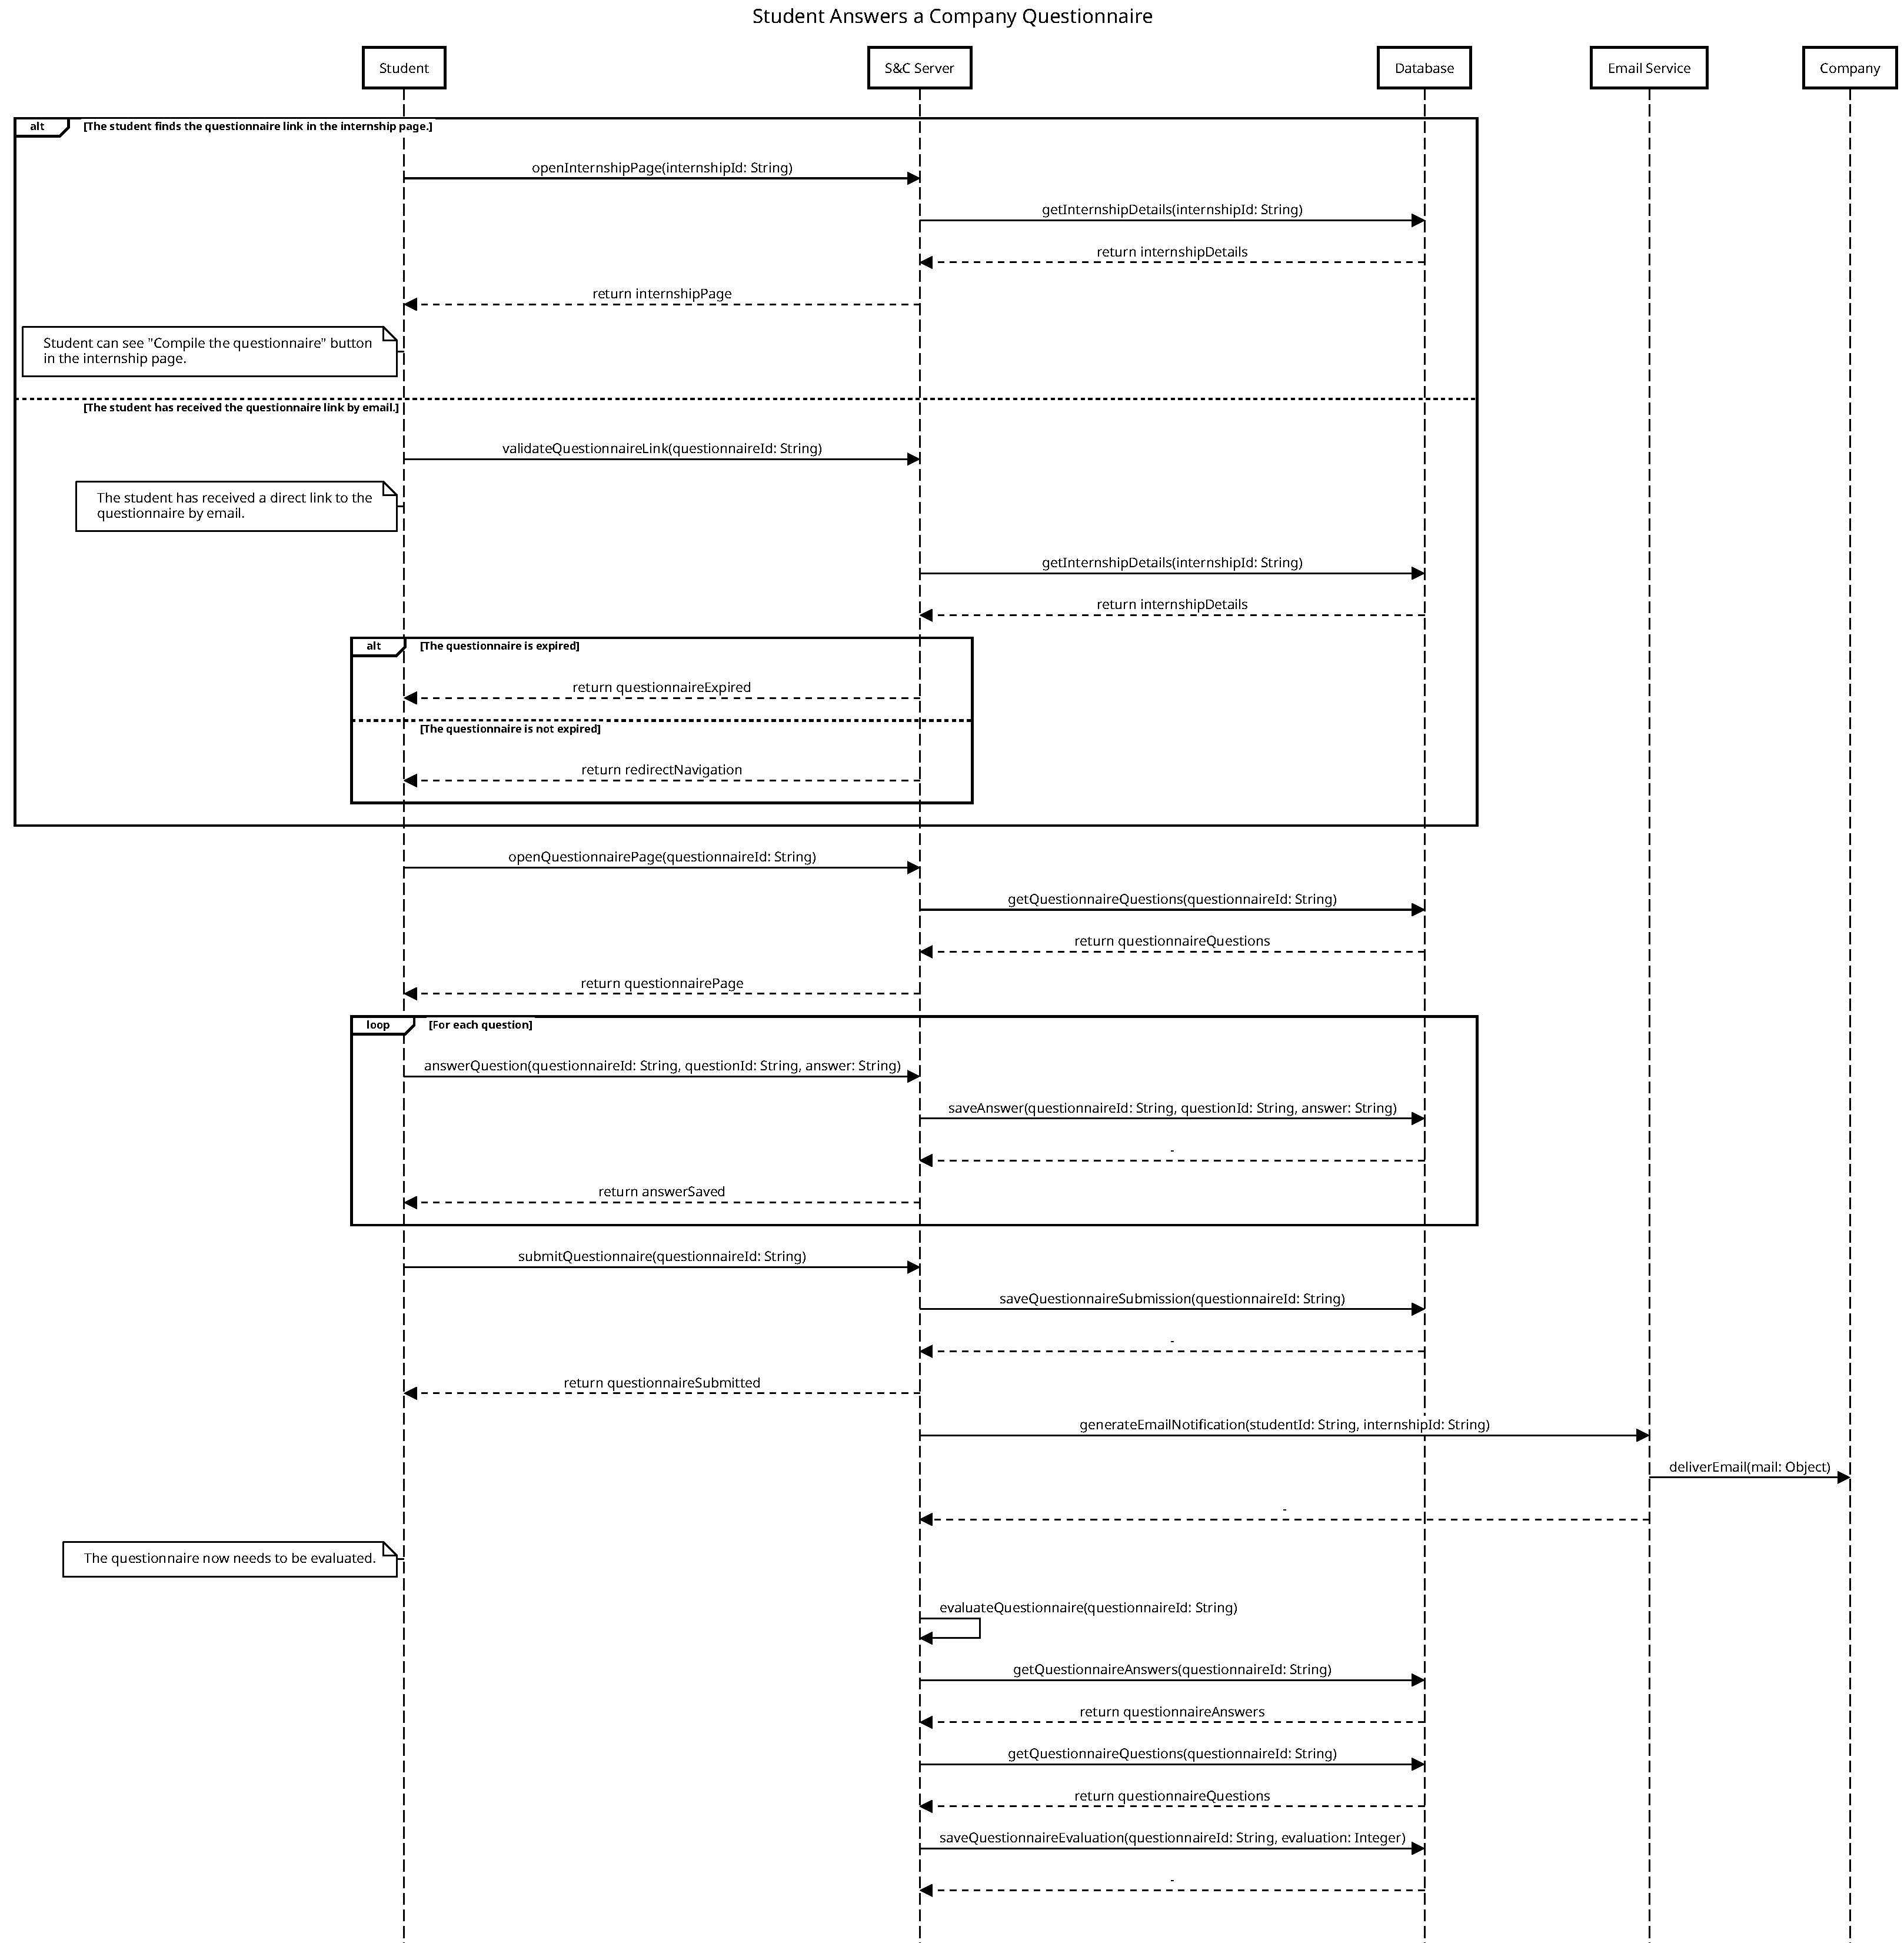
\includegraphics[width=1.0\textwidth]{Images/UC_5.pdf}
    \caption{Student Answers a Company Questionnaire - Use Case Diagram}
    \label{fig:use-case-diagram-5}
\end{figure}

% 6	

\subsubsection{UC06: Student creates a complaints}
\label{subsubsec:student-creates-a-complaints}

\begin{center}
    \begin{longtable}{|l|p{0.75\linewidth}|}
        \hline
        \textbf{Actors:}           & ST, (opt) UN                                                                                                                     \\
        \hline
        \textbf{Entry Conditions:} & The ST is correctly logged in. The ST had decided to create a complaint about the internship he's doing.                         \\
        \hline
        \textbf{Flow of Events:}   & \begin{enumerate}
                                         \item ST clicks on the "Create Complaint" button.
                                         \item S\&C send to the ST a form to fill with the complaint details.
                                         \item ST fills the form and submits it.
                                         \item S\&C stores the complaint in the database.
                                         \item S\&C request to the Emailing system to send an email to the UN about a new complaint about an internship of one of it's ST.
                                         \item The Emailing system sends the email to the UN.
                                         \item S\&C notifies the ST that the complaint was successfully submitted.
                                         \item (opt) UN acknowledges the complaint.
                                         \item (opt) S\&C change the status of the complaint to "Acknowledged".
                                     \end{enumerate} \\
        \hline
        \textbf{Exit Conditions:}  & ST receive the confirmation of the complaint being saved correctly.                                                              \\
        \hline
        \textbf{Exceptions:}       & S\&C generated an internal error.                                                                                                \\
        \hline
    \end{longtable}
\end{center}

\begin{figure}[H]
    \centering
    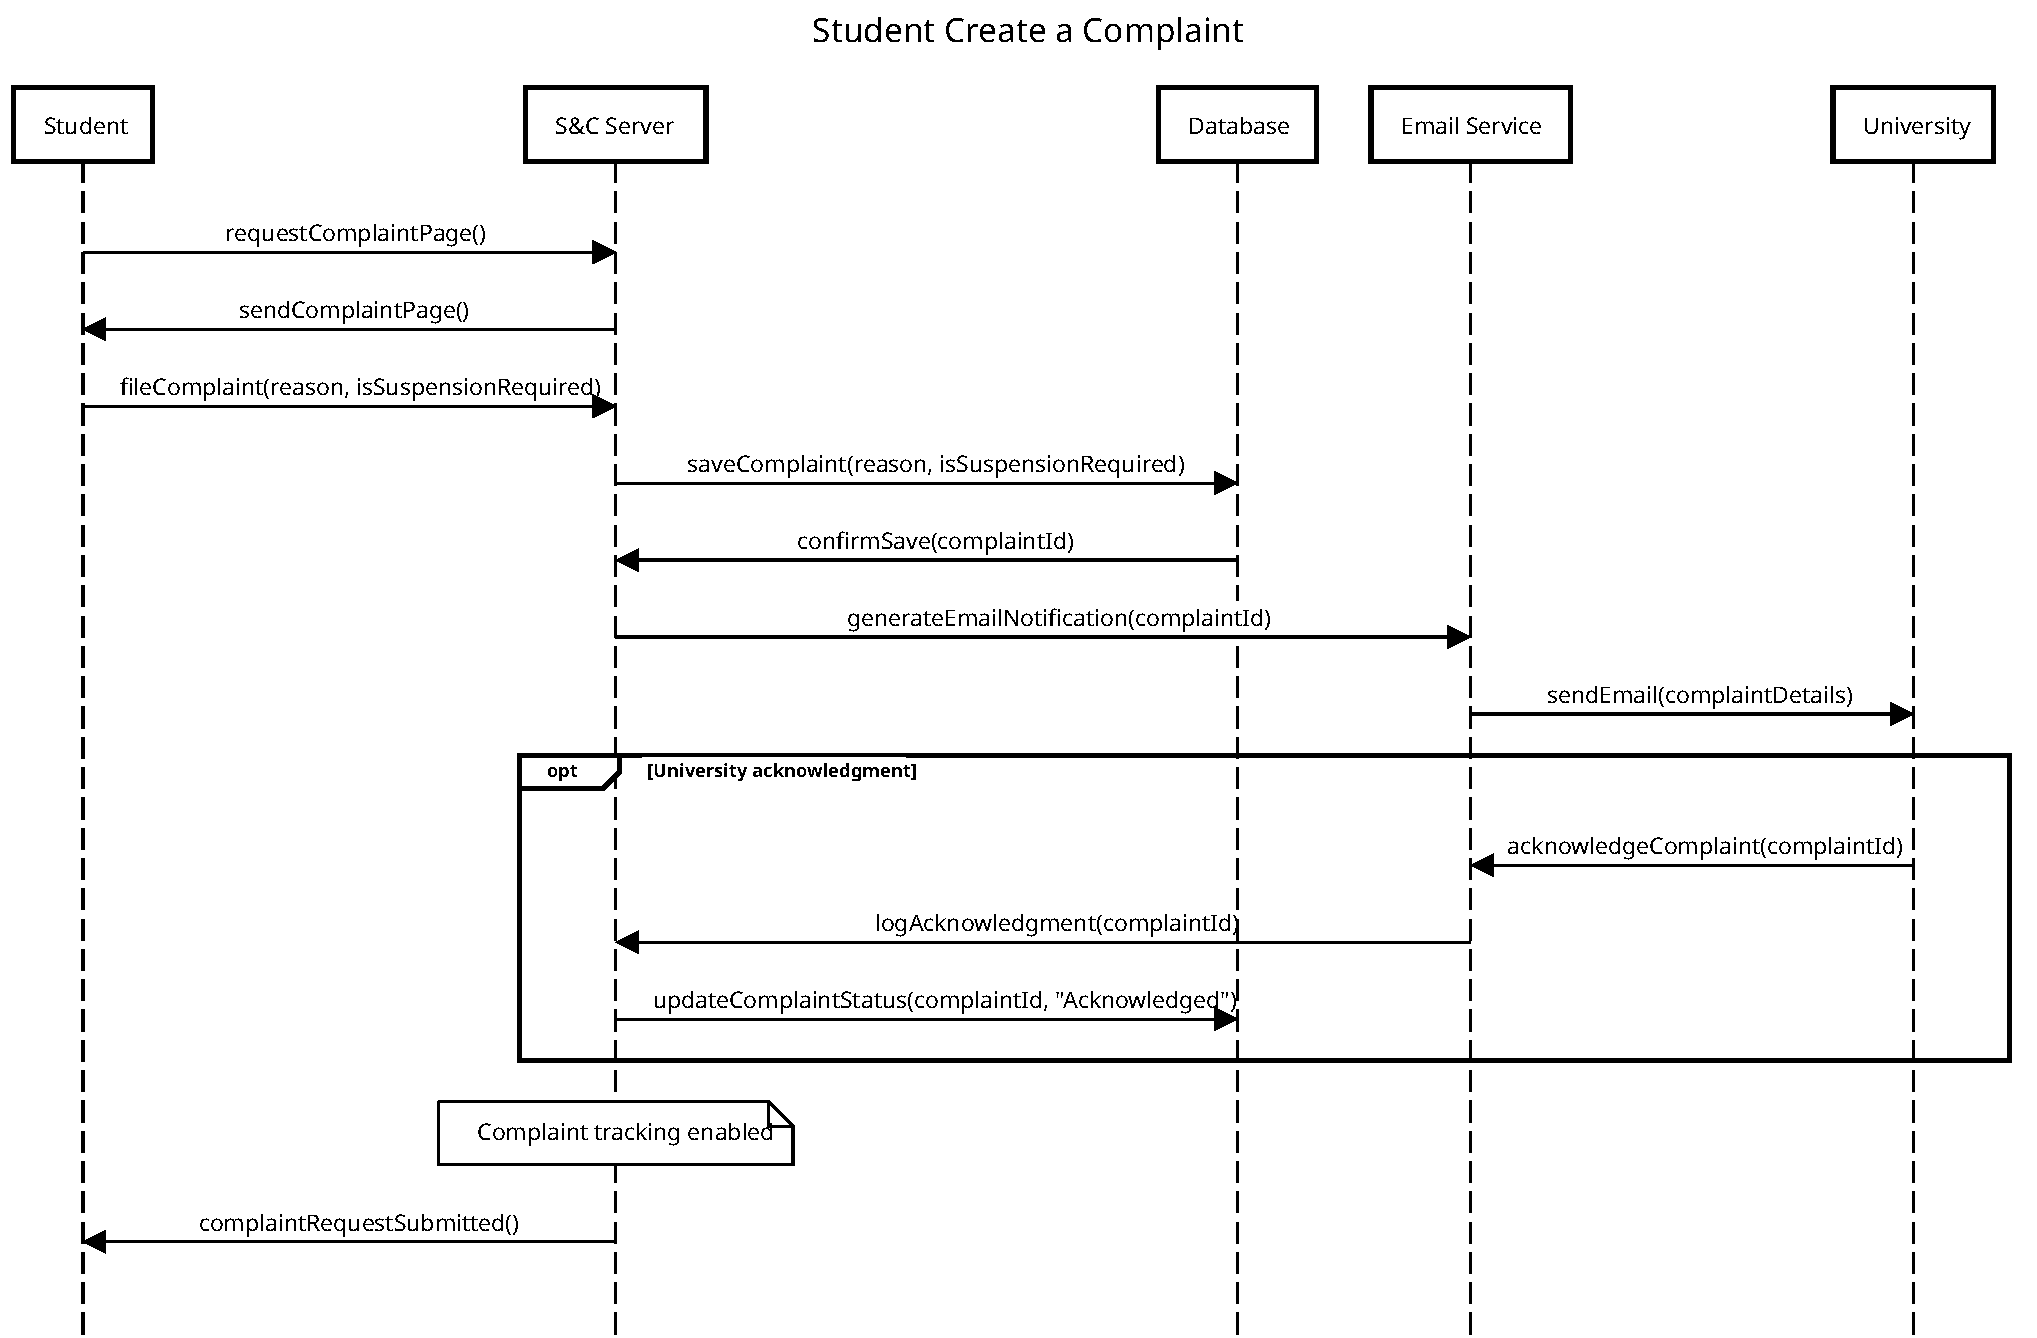
\includegraphics[width=1.0\textwidth]{Images/UC_6.pdf}
    \caption{Student Creates a Complaint - Use Case Diagram}
    \label{fig:use-case-diagram-6}
\end{figure}

% 7

\subsubsection{UC07: Student answers questionnaire at internship completion}
\label{subsubsec:student-answers-questionnaire-at-internship-completion}

\begin{center}
    \begin{longtable}{|l|p{0.75\linewidth}|}
        \hline
        \textbf{Actors:}           & ST                                                                                                     \\
        \hline
        \textbf{Entry Conditions:} & ST is correctly logged in. The related internship has ended.                                           \\
        \hline
        \textbf{Flow of Events:}   & \begin{enumerate}
                                         \item ST clicks on the "Fill Questionnaire" button.
                                         \item S\&C fetch the questionnaire from its database.
                                         \item S\&C gives the questionnaire to the ST.
                                         \item ST fills the questions and submits them.
                                         \item S\&C stores the answers to the questionnaire in the database.
                                         \item S\&C feeds the answers of the questionnaire to the suggestion system to learn from this new data.
                                     \end{enumerate} \\
        \hline
        \textbf{Exit Conditions:}  & ST receive the confirmation of the questionnaire being saved correctly.                                \\
        \hline
        \textbf{Exceptions:}       & Possible invalid formats for the answers submitted by the ST.                                          \\
        \hline
    \end{longtable}
\end{center}

\begin{figure}[H]
    \centering
    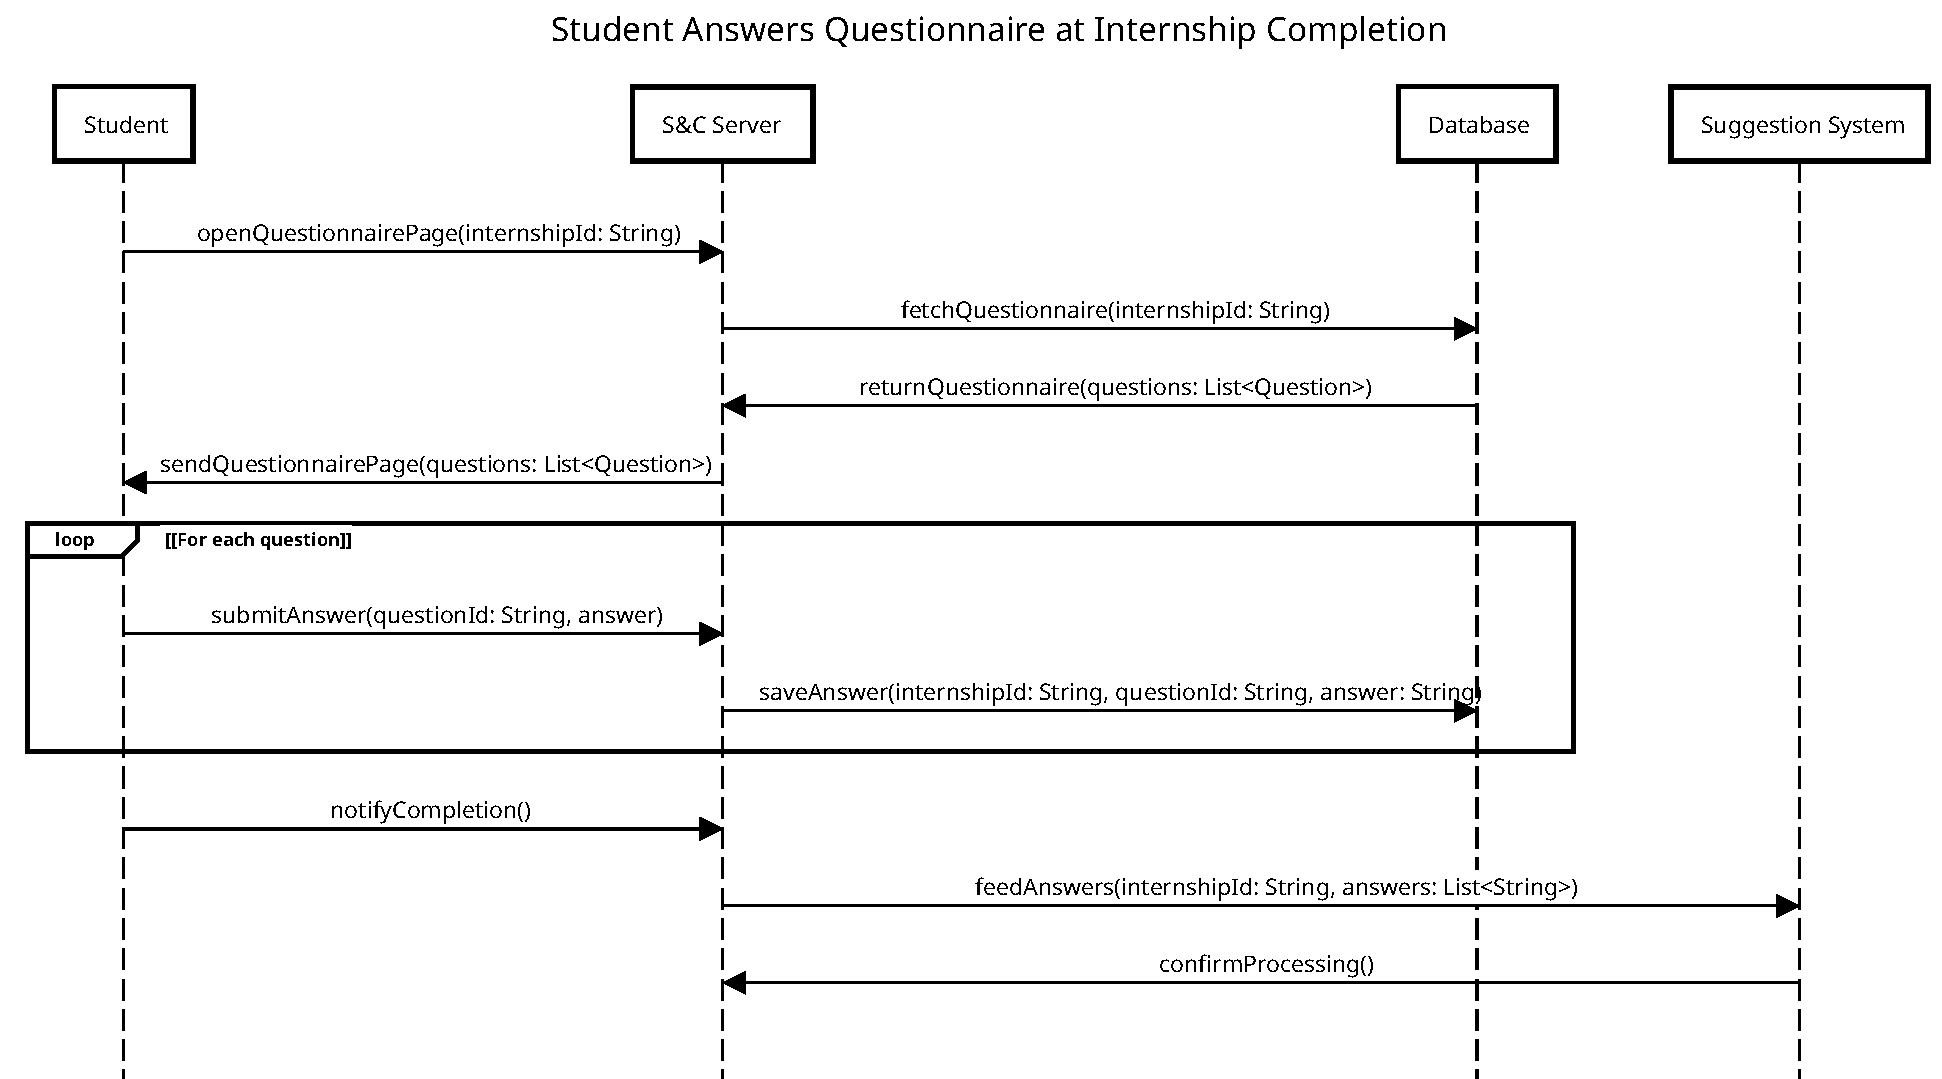
\includegraphics[width=1.0\textwidth]{Images/UC_7.pdf}
    \caption{Student Answers Questionnaire at Internship Completion - Use Case Diagram}
    \label{fig:use-case-diagram-7}
\end{figure}

\pagebreak

% 8

\subsubsection{UC08: Company login}
\label{subsubsec:company-login}

\begin{center}
    \begin{longtable}{|l|p{0.75\linewidth}|}
        \hline
        \textbf{Actors:}           & CO                                                                                            \\
        \hline
        \textbf{Entry Conditions:} & CO has received the credentials by S\&C staff after the payment for the usage of the Website. \\
        \hline
        \textbf{Flow of Events:}   & \begin{enumerate}
                                         \item CO search the URL of S\&C login page.
                                         \item S\&C send to CO the login web page.
                                         \item CO inserts the username and password received.
                                         \item S\&C validates the credentials.
                                         \item S\&C sends the CO to the CO dashboard.
                                     \end{enumerate}                                           \\
        \hline
        \textbf{Exit Conditions:}  & CO is redirected to the CO dashboard.                                                         \\
        \hline
        \textbf{Exceptions:}       &
        \begin{itemize}
            \item The credentials are wrong.
            \item The CO is was blocked by the S\&C staff after a violation of the platform guidelines.
            \item S\&C generated an internal error.
        \end{itemize}                                 \\
        \hline
    \end{longtable}
\end{center}

\begin{figure}[H]
    \centering
    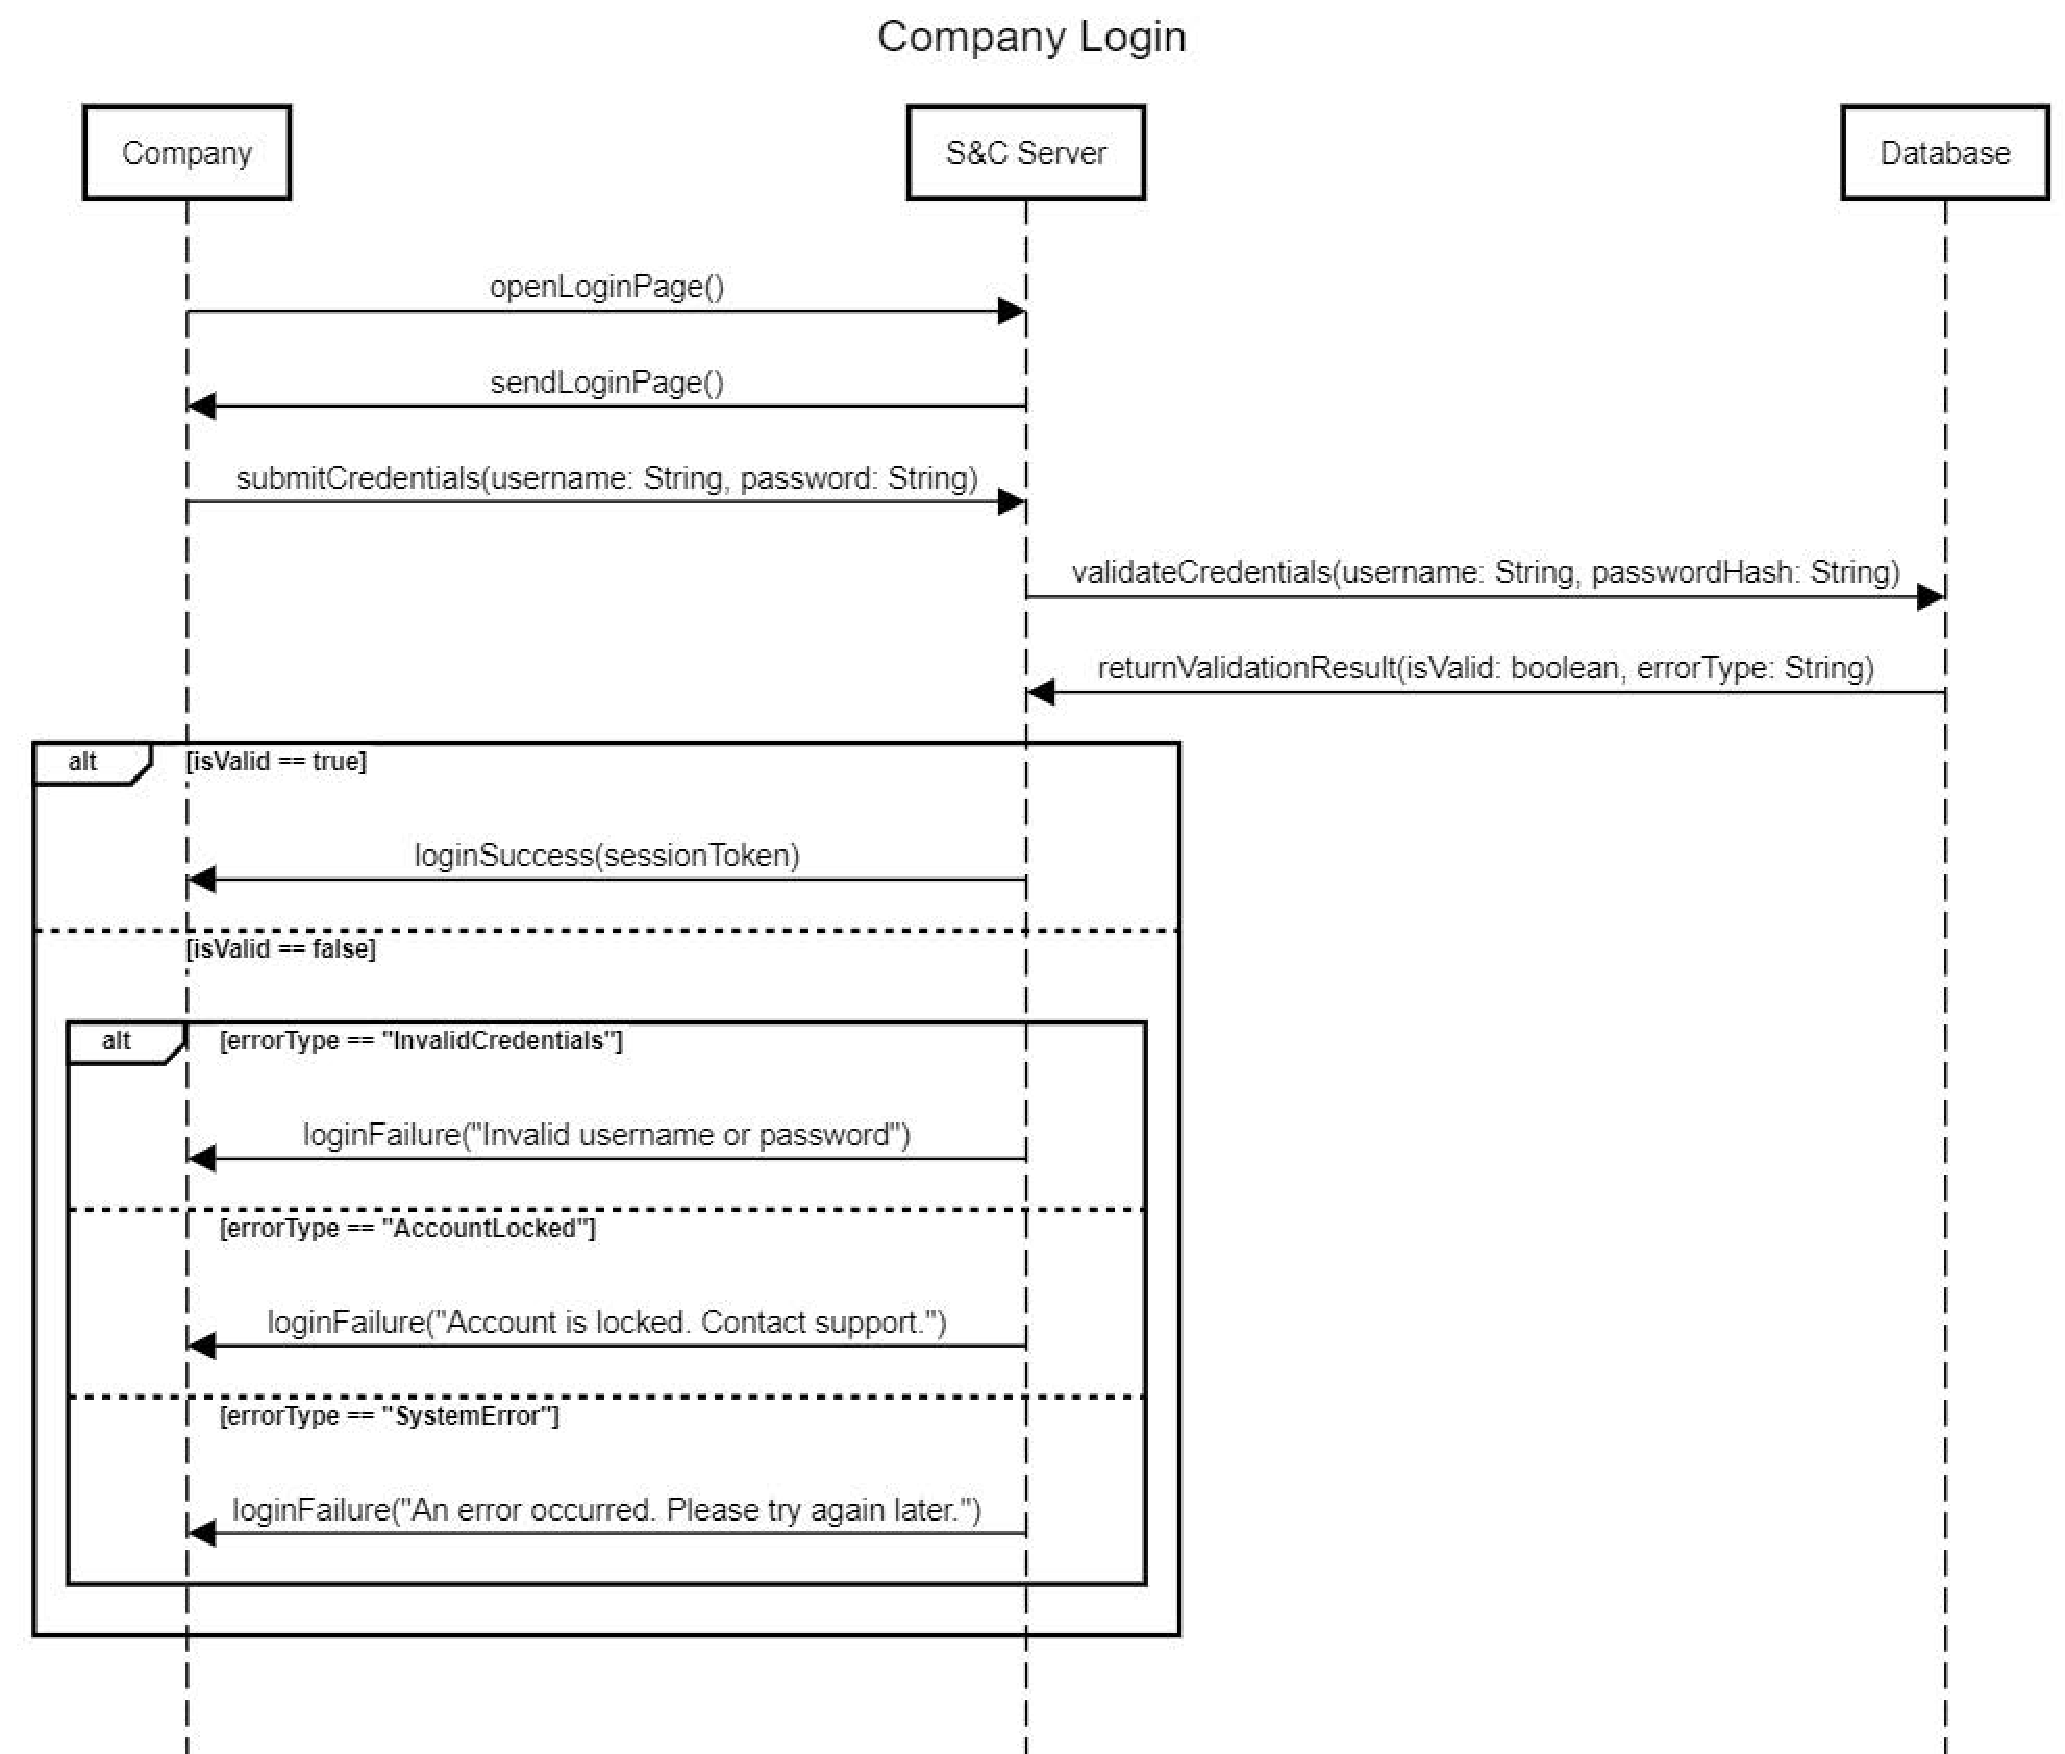
\includegraphics[width=1.0\textwidth]{Images/UC_8.pdf}
    \caption{Company Login - Use Case Diagram}
    \label{fig:use-case-diagram-8}
\end{figure}

% 9

\subsubsection{UC09: Company creates an internship announcement}
\label{subsubsec:company-creates-an-internship-announcement}

\begin{center}
    \begin{longtable}{|l|p{0.75\linewidth}|}
        \hline
        \textbf{Actors:}           & CO                                                                                                                                                 \\                                                                                       \\
        \hline
        \textbf{Entry Conditions:} & CO is correctly logged in.                                                                                                                         \\
        \hline
        \textbf{Flow of Events:}   & \begin{enumerate}
                                         \item CO opens the page "Create Internship".
                                         \item CO compiles all the required fields for the internship.
                                         \item S\&C saves the internship in the database, it is now visible to students.
                                         \item CO can at any time decide to open the internship and start receiving applications. CO is required to provide a Deadline for the applications.
                                         \item S\&C suggestion system provides to CO a set of candidates that could be suitable for the internship.
                                         \item When the deadline is reached, the internship is automatically closed.
                                     \end{enumerate} \\
        \hline
        \textbf{Exit Conditions:}  & CO has successfully created an internship announcement or a partial version was saved.                                                             \\
        \hline
        \textbf{Exceptions:}       & S\&C generated an internal error.                                                                                                                  \\
        \hline
    \end{longtable}
\end{center}

\begin{figure}[H]
    \centering
    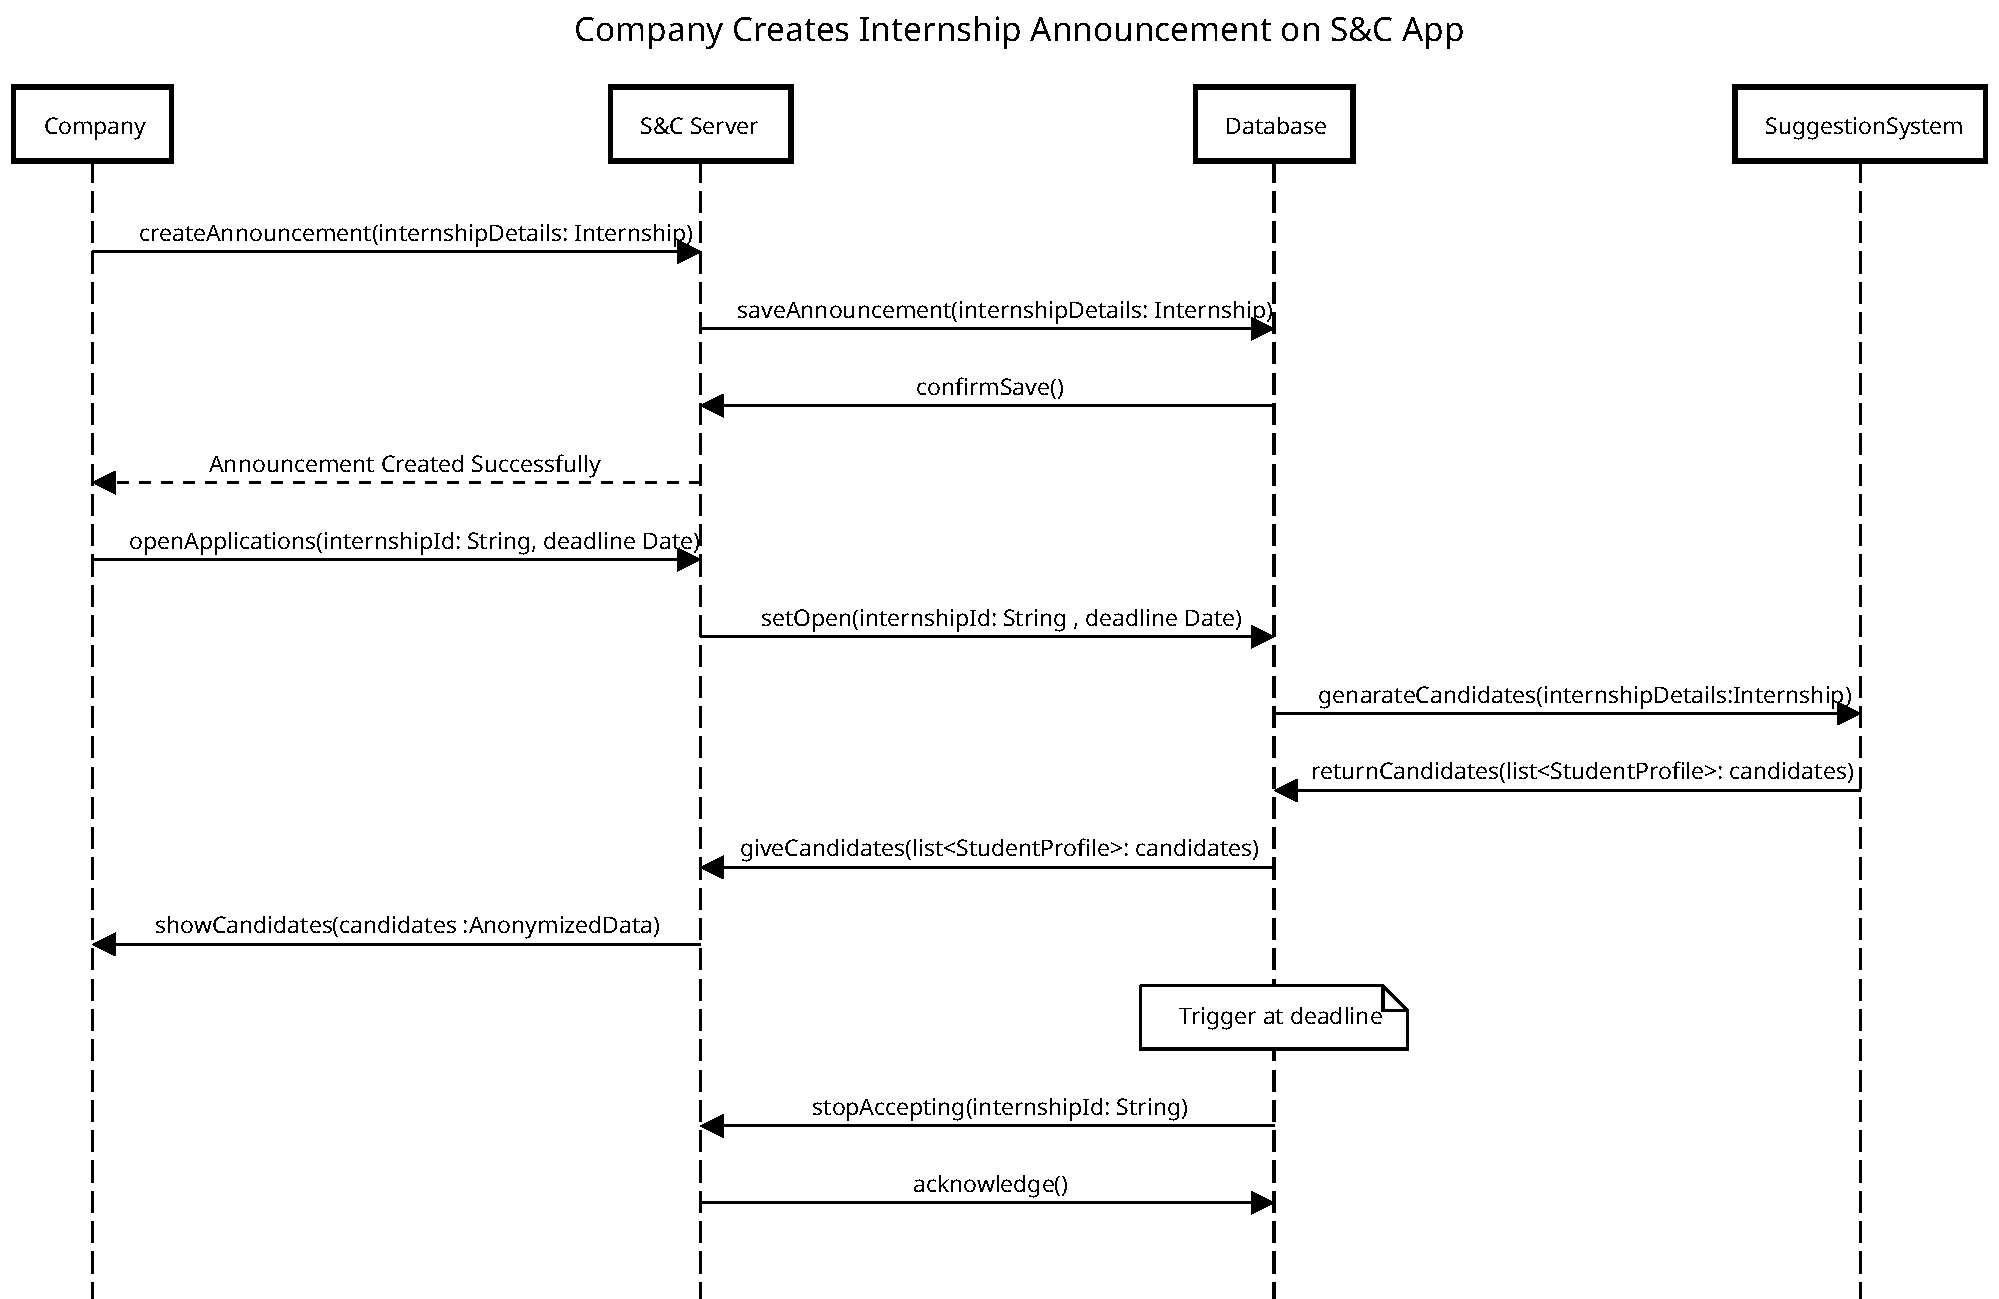
\includegraphics[width=1.0\textwidth]{Images/UC_9.pdf}
    \caption{Company Creates an Internship Announcement - Use Case Diagram}
    \label{fig:use-case-diagram-9}
\end{figure}

% 10

\subsubsection{UC10: Company looks for extra potential candidates through the recommendation system}
\label{subsubsec:company-looks-for-extra-potential-candidates-through-the-recommendation-system}

\begin{center}
    \begin{longtable}{|l|p{0.75\linewidth}|}
        \hline
        \textbf{Actors:}           & CO, ST                                                                                                                \\
        \hline
        \textbf{Entry Conditions:} & CO is correctly logged in. CO has published an internship listing.                                                    \\
        \hline
        \textbf{Flow of Events:}   & \begin{enumerate}
                                         \item CO selects an internship to view the details from the "My Internships" page.
                                         \item S\&C fetch the internship details from the database.
                                         \item S\&C shows the internship details to the CO.
                                         \item CO clicks on the "Applicants" button.
                                         \item S\&C fetch the applicants from the database.
                                         \item S\&C shows the applicants to the CO.
                                         \item CO clicks on "Recommended Candidates" button.
                                         \item (opt. 1) S\&C fetch the recommended candidates from the database.
                                         \item (opt. 2) The list of recommended candidates must be updated.
                                               \begin{enumerate}
                      \item The recommendation system fetches information about the internship.
                      \item The recommendation system computes a set of filters used to find the best candidates.
                      \item The recommendation system fetches the candidates from the database using the filters.
                      \item The recommendation system stores the list of "preferred" candidates in the database.
                  \end{enumerate}
                                         \item S\&C shows the recommended candidates to the CO.
                                         \item CO selects a candidate to view the details of.
                                         \item S\&C fetch the candidate details from the database.
                                         \item S\&C shows the candidate details to the CO.
                                         \item CO, if interested, can "suggests" the internship to the ST by clicking on the "Suggests this Internship" button.
                                         \item S\&C sends the ST a notification email about the internship suggestion.
                                         \item S\&C stores the CO interest for this particular ST.
                                     \end{enumerate} \\
        \hline
        \textbf{Exit Conditions:}  & CO has increased the number of potential candidates for the internship.                                               \\
        \hline
        \textbf{Exceptions:}       & S\&C generated an internal error.                                                                                     \\
        \hline
    \end{longtable}
\end{center}

\begin{figure}[H]
    \centering
    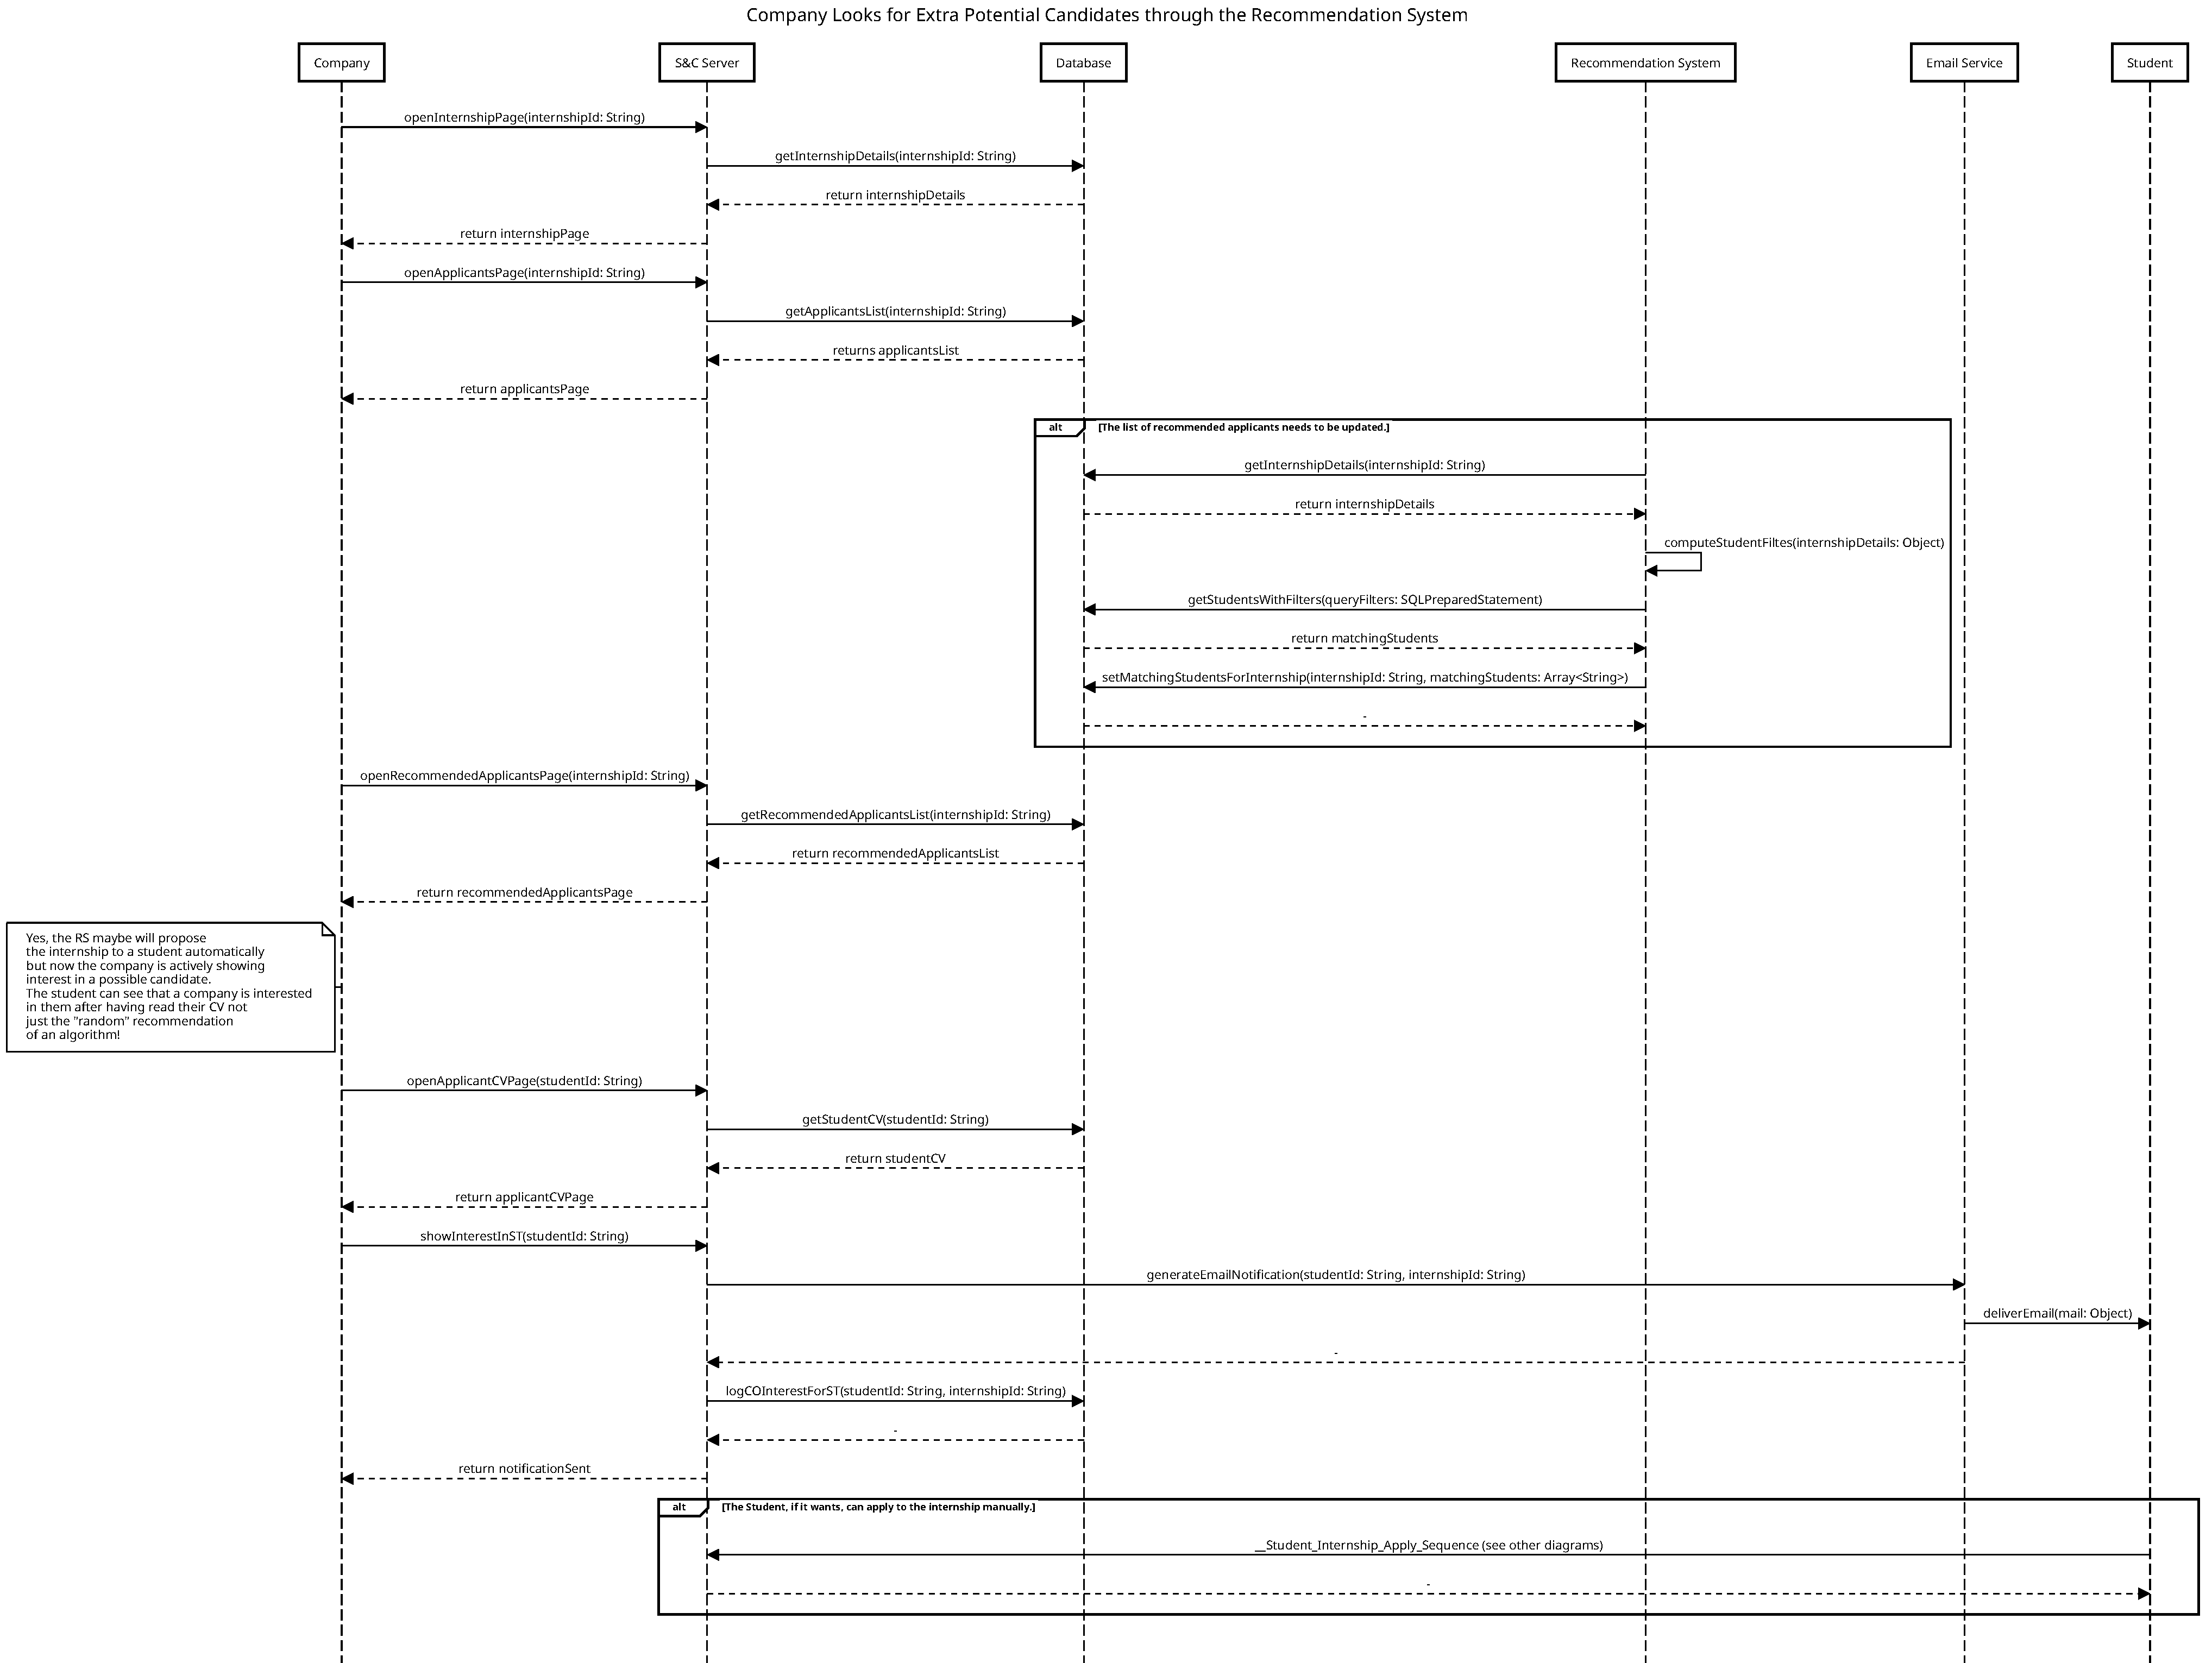
\includegraphics[width=1.0\textwidth]{Images/UC_10.pdf}
    \caption{Company Looks for Extra Potential Candidates through the Recommendation System - Use Case Diagram}
    \label{fig:use-case-diagram-10}
\end{figure}

% 11

\subsubsection{UC11: Company creates a questionnaire for the applicants}
\label{subsubsec:company-creates-a-questionnaire-for-the-applicants}

\begin{center}
    \begin{longtable}{|l|p{0.75\linewidth}|}
        \hline
        \textbf{Actors:}           & CO                                                                                                        \\
        \hline
        \textbf{Entry conditions:} & CO is correctly logged in. An internship has reached the deadline and now has to evaluate the candidates. \\                                                                                                  \\
        \hline
        \textbf{Flow of Events:}   & \begin{enumerate}
                                         \item CO visits the "My Internships" page.
                                         \item S\&C fetch the internships from the database.
                                         \item S\&C shows the internships to the CO.
                                         \item CO selects an internship to view the details.
                                         \item S\&C fetch the internship details from the database.
                                         \item S\&C shows the internship details to the CO.
                                         \item CO clicks on the "Create Questionnaire" button.
                                         \item S\&C sends the questionnaire template to the CO.
                                         \item CO fills the questionnaire  with relevant questions.
                                         \item S\&C stores the questionnaire in the database.
                                         \item S\&C notifies the CO that the questionnaire was successfully created.
                                     \end{enumerate}                                \\
        \hline
        \textbf{Exit Conditions:}  & CO has successfully created a questionnaire for the applicants or a partial version has been saved.       \\
        \hline
        \textbf{Exceptions:}       & S\&C generated an internal error.                                                                         \\
        \hline
    \end{longtable}
\end{center}

\begin{figure}[H]
    \centering
    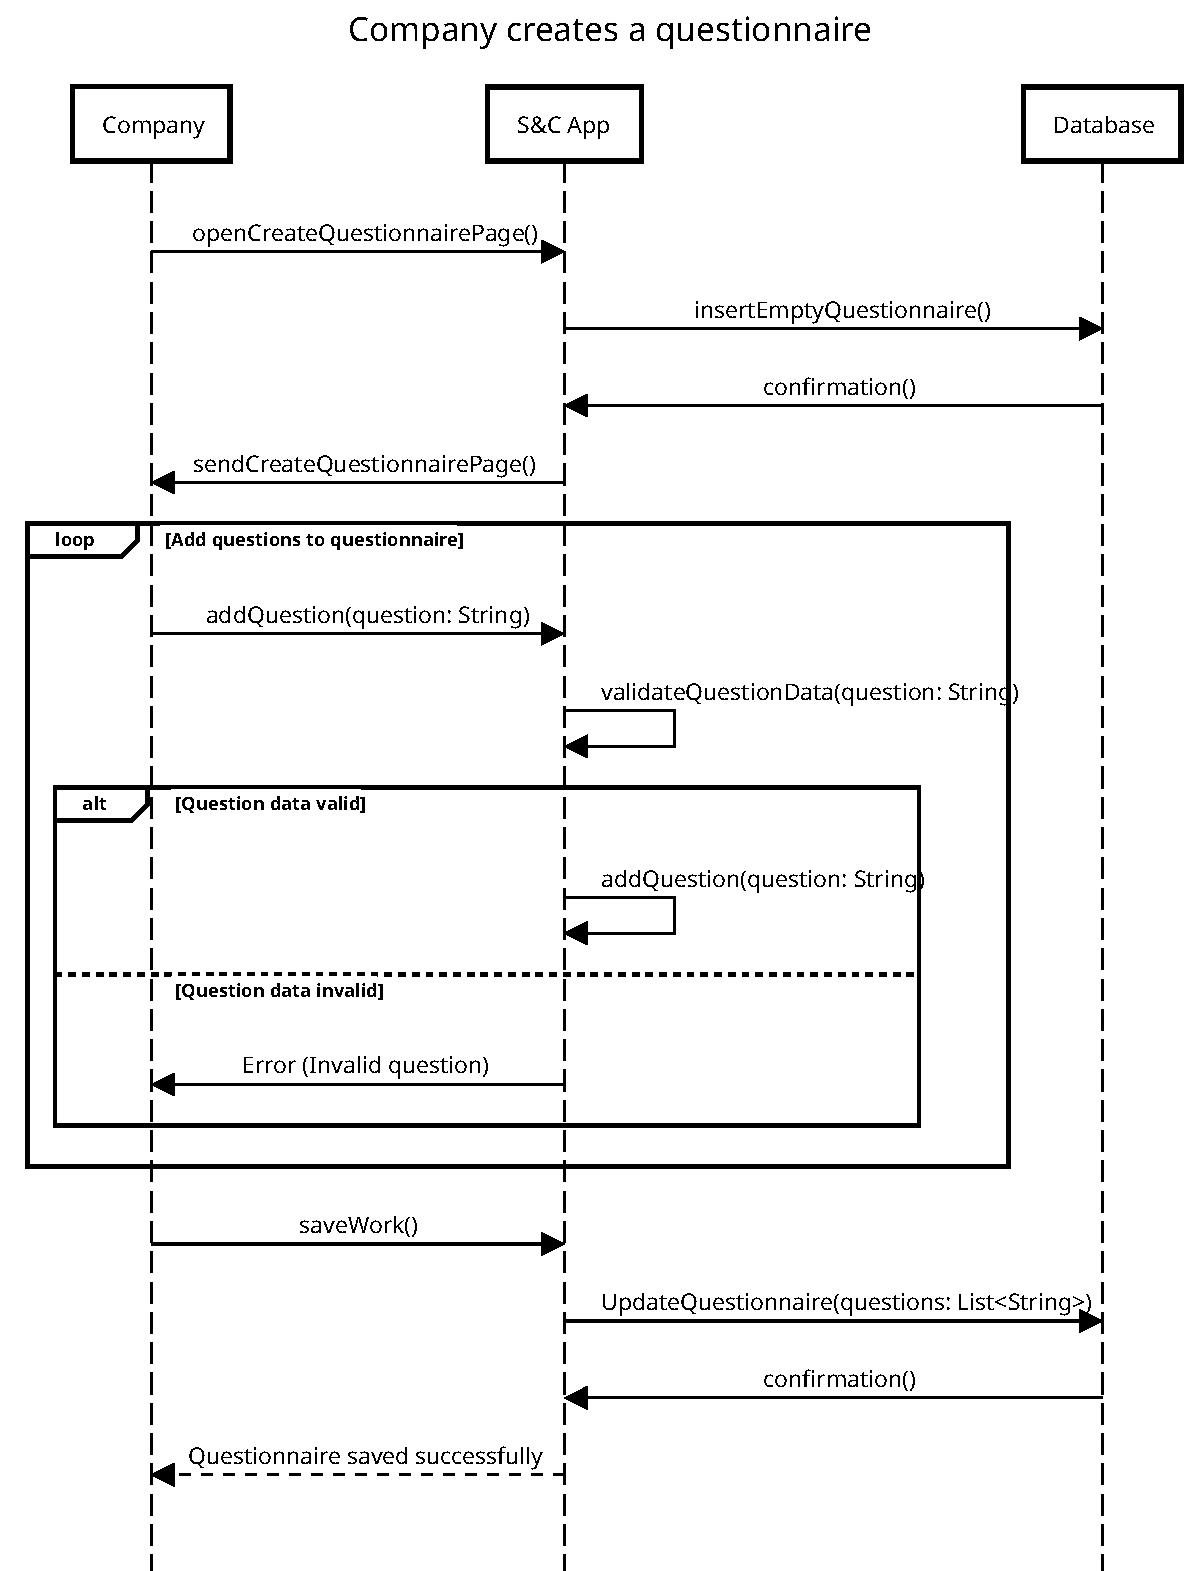
\includegraphics[width=1.0\textwidth]{Images/UC_11.pdf}
    \caption{Company Creates a Questionnaire for the Applicants - Use Case Diagram}
    \label{fig:use-case-diagram-11}
\end{figure}

% 12

\subsubsection{UC12: Company selects applicant student for its internship}
\label{subsubsec:company-select-applicant-student-for-its-internship}

\begin{center}
    \begin{longtable}{|l|p{0.75\linewidth}|}
        \hline
        \textbf{Actors:}           & CO                                                                                                                      \\
        \hline
        \textbf{Entry Conditions:} & CO is correctly logged in, has already created an internship listing, and has received applications from STs.
        CO has already loaded the questionnaire for the STs.CO is correctly logged in. CO has published an internship listing.                               \\
        \hline
        \textbf{Flow of Events:}   & \begin{enumerate}
                                         \item CO request the page that shows the applications for his internship.
                                         \item S\&C fetches the applications from the database.
                                         \item S\&C shows the applications to the CO.
                                         \item CO selects the STs he wants to send the questionnaire.
                                         \item S\&C store the selection of STs linked to the internship.
                                         \item CO confirm the questionnaire to be sent to the selected STs.
                                         \item S\&C notifies the selected STs that they have a questionnaire to fill, inherent to the CO's internship, via email.
                                     \end{enumerate} \\
        \hline
        \textbf{Exit Conditions:}  & CO receives a confirmation that S\&C has sent the questionnaire to the selected STs.                                    \\
        \hline
        \textbf{Exceptions:}       & S\&C generated an internal error.                                                                                       \\
        \hline
    \end{longtable}
\end{center}

\begin{figure}[H]
    \centering
    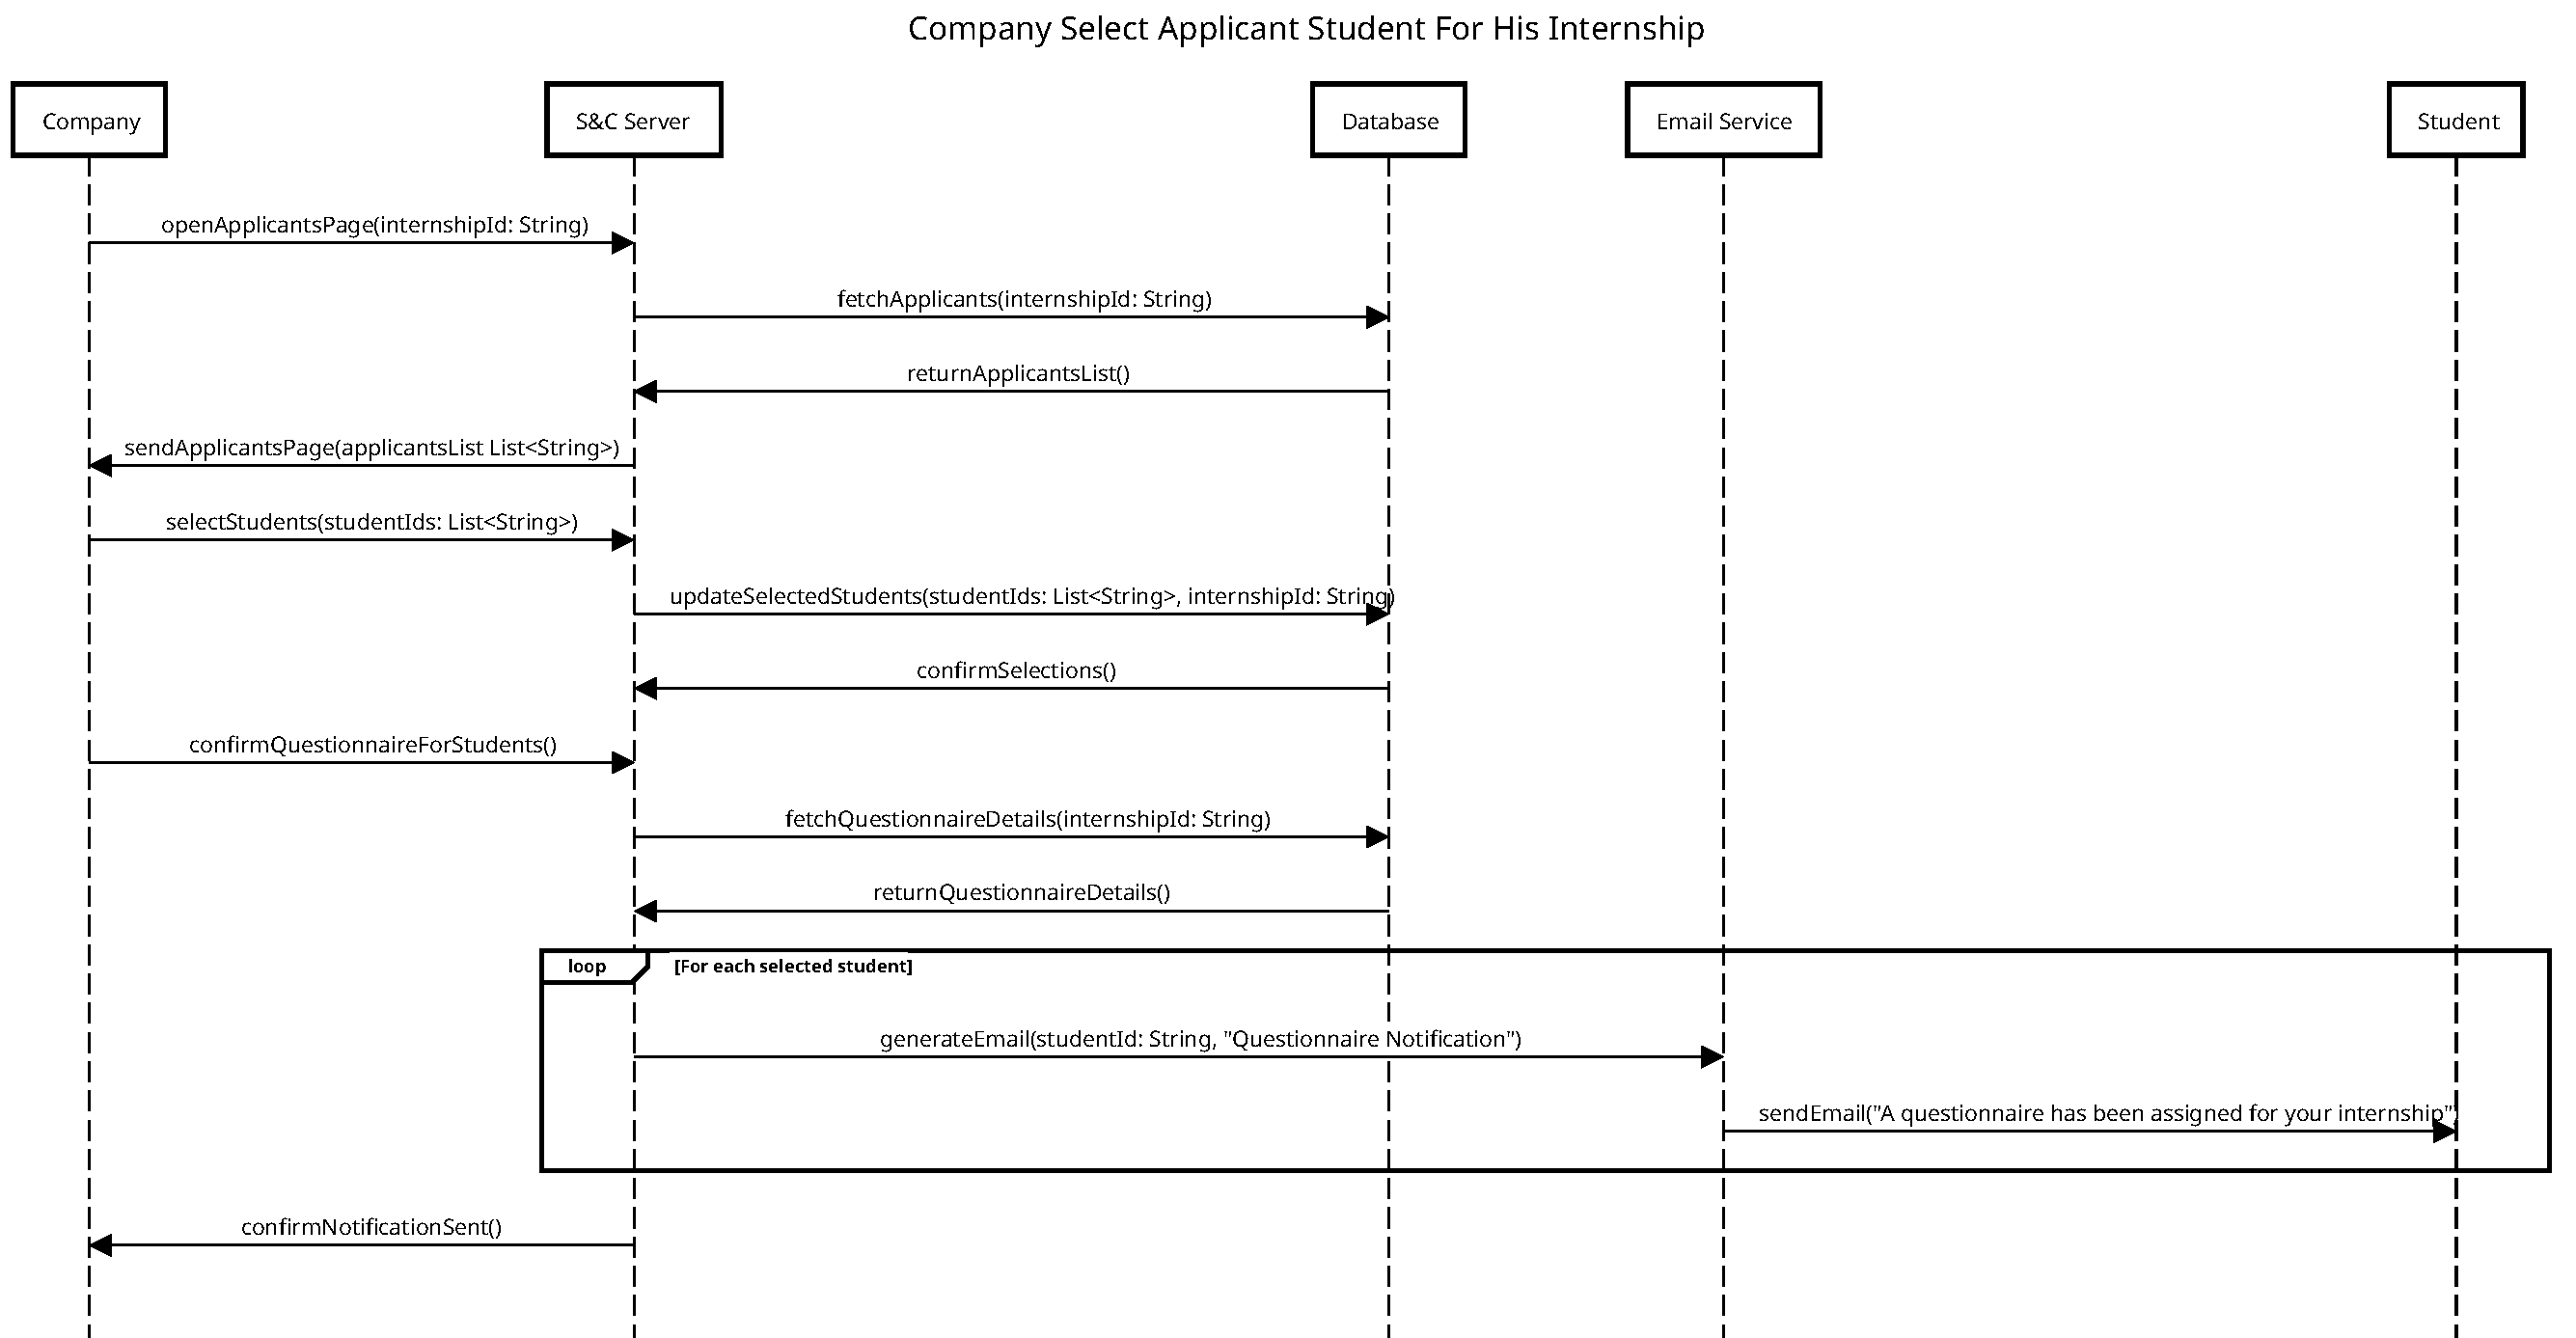
\includegraphics[width=1.0\textwidth]{Images/UC_12.pdf}
    \caption{Company Selects Applicant Student for its Internship - Use Case Diagram}
    \label{fig:use-case-diagram-12}
\end{figure}

% 13

\subsubsection{UC13: Company creates a complaints}
\label{subsubsec:company-creates-a-complaints}

\begin{center}
    \begin{longtable}{|l|p{0.75\linewidth}|}
        \hline
        \textbf{Actors:}           & CO, (opt) UN                                                                                                                     \\
        \hline
        \textbf{Entry Conditions:} & CO is correctly logged in. CO had decided to create a complaint about the internship it's holding.                               \\
        \hline
        \textbf{Flow of Events:}   & \begin{enumerate}
                                         \item CO clicks on the "Create Complaint" button.
                                         \item S\&C send to the CO a form to fill with the complaint details.
                                         \item CO fills the form and submits it.
                                         \item S\&C stores the complaint in the database.
                                         \item S\&C request to the Emailing system to send an email to the UN about a new complaint about an internship of one of it's ST.
                                         \item The Emailing system sends the email to the UN.
                                         \item S\&C notifies the CO that the complaint was successfully submitted.
                                         \item (opt) UN acknowledges the complaint.
                                         \item (opt) S\&C change the status of the complaint to "Acknowledged".
                                     \end{enumerate} \\
        \hline
        \textbf{Exit Conditions:}  & CO has increased the number of potential candidates for the internship.                                                          \\
        \hline
        \textbf{Exceptions:}       & S\&C generated an internal error.                                                                                                \\
        \hline
    \end{longtable}
\end{center}

\begin{figure}[H]
    \centering
    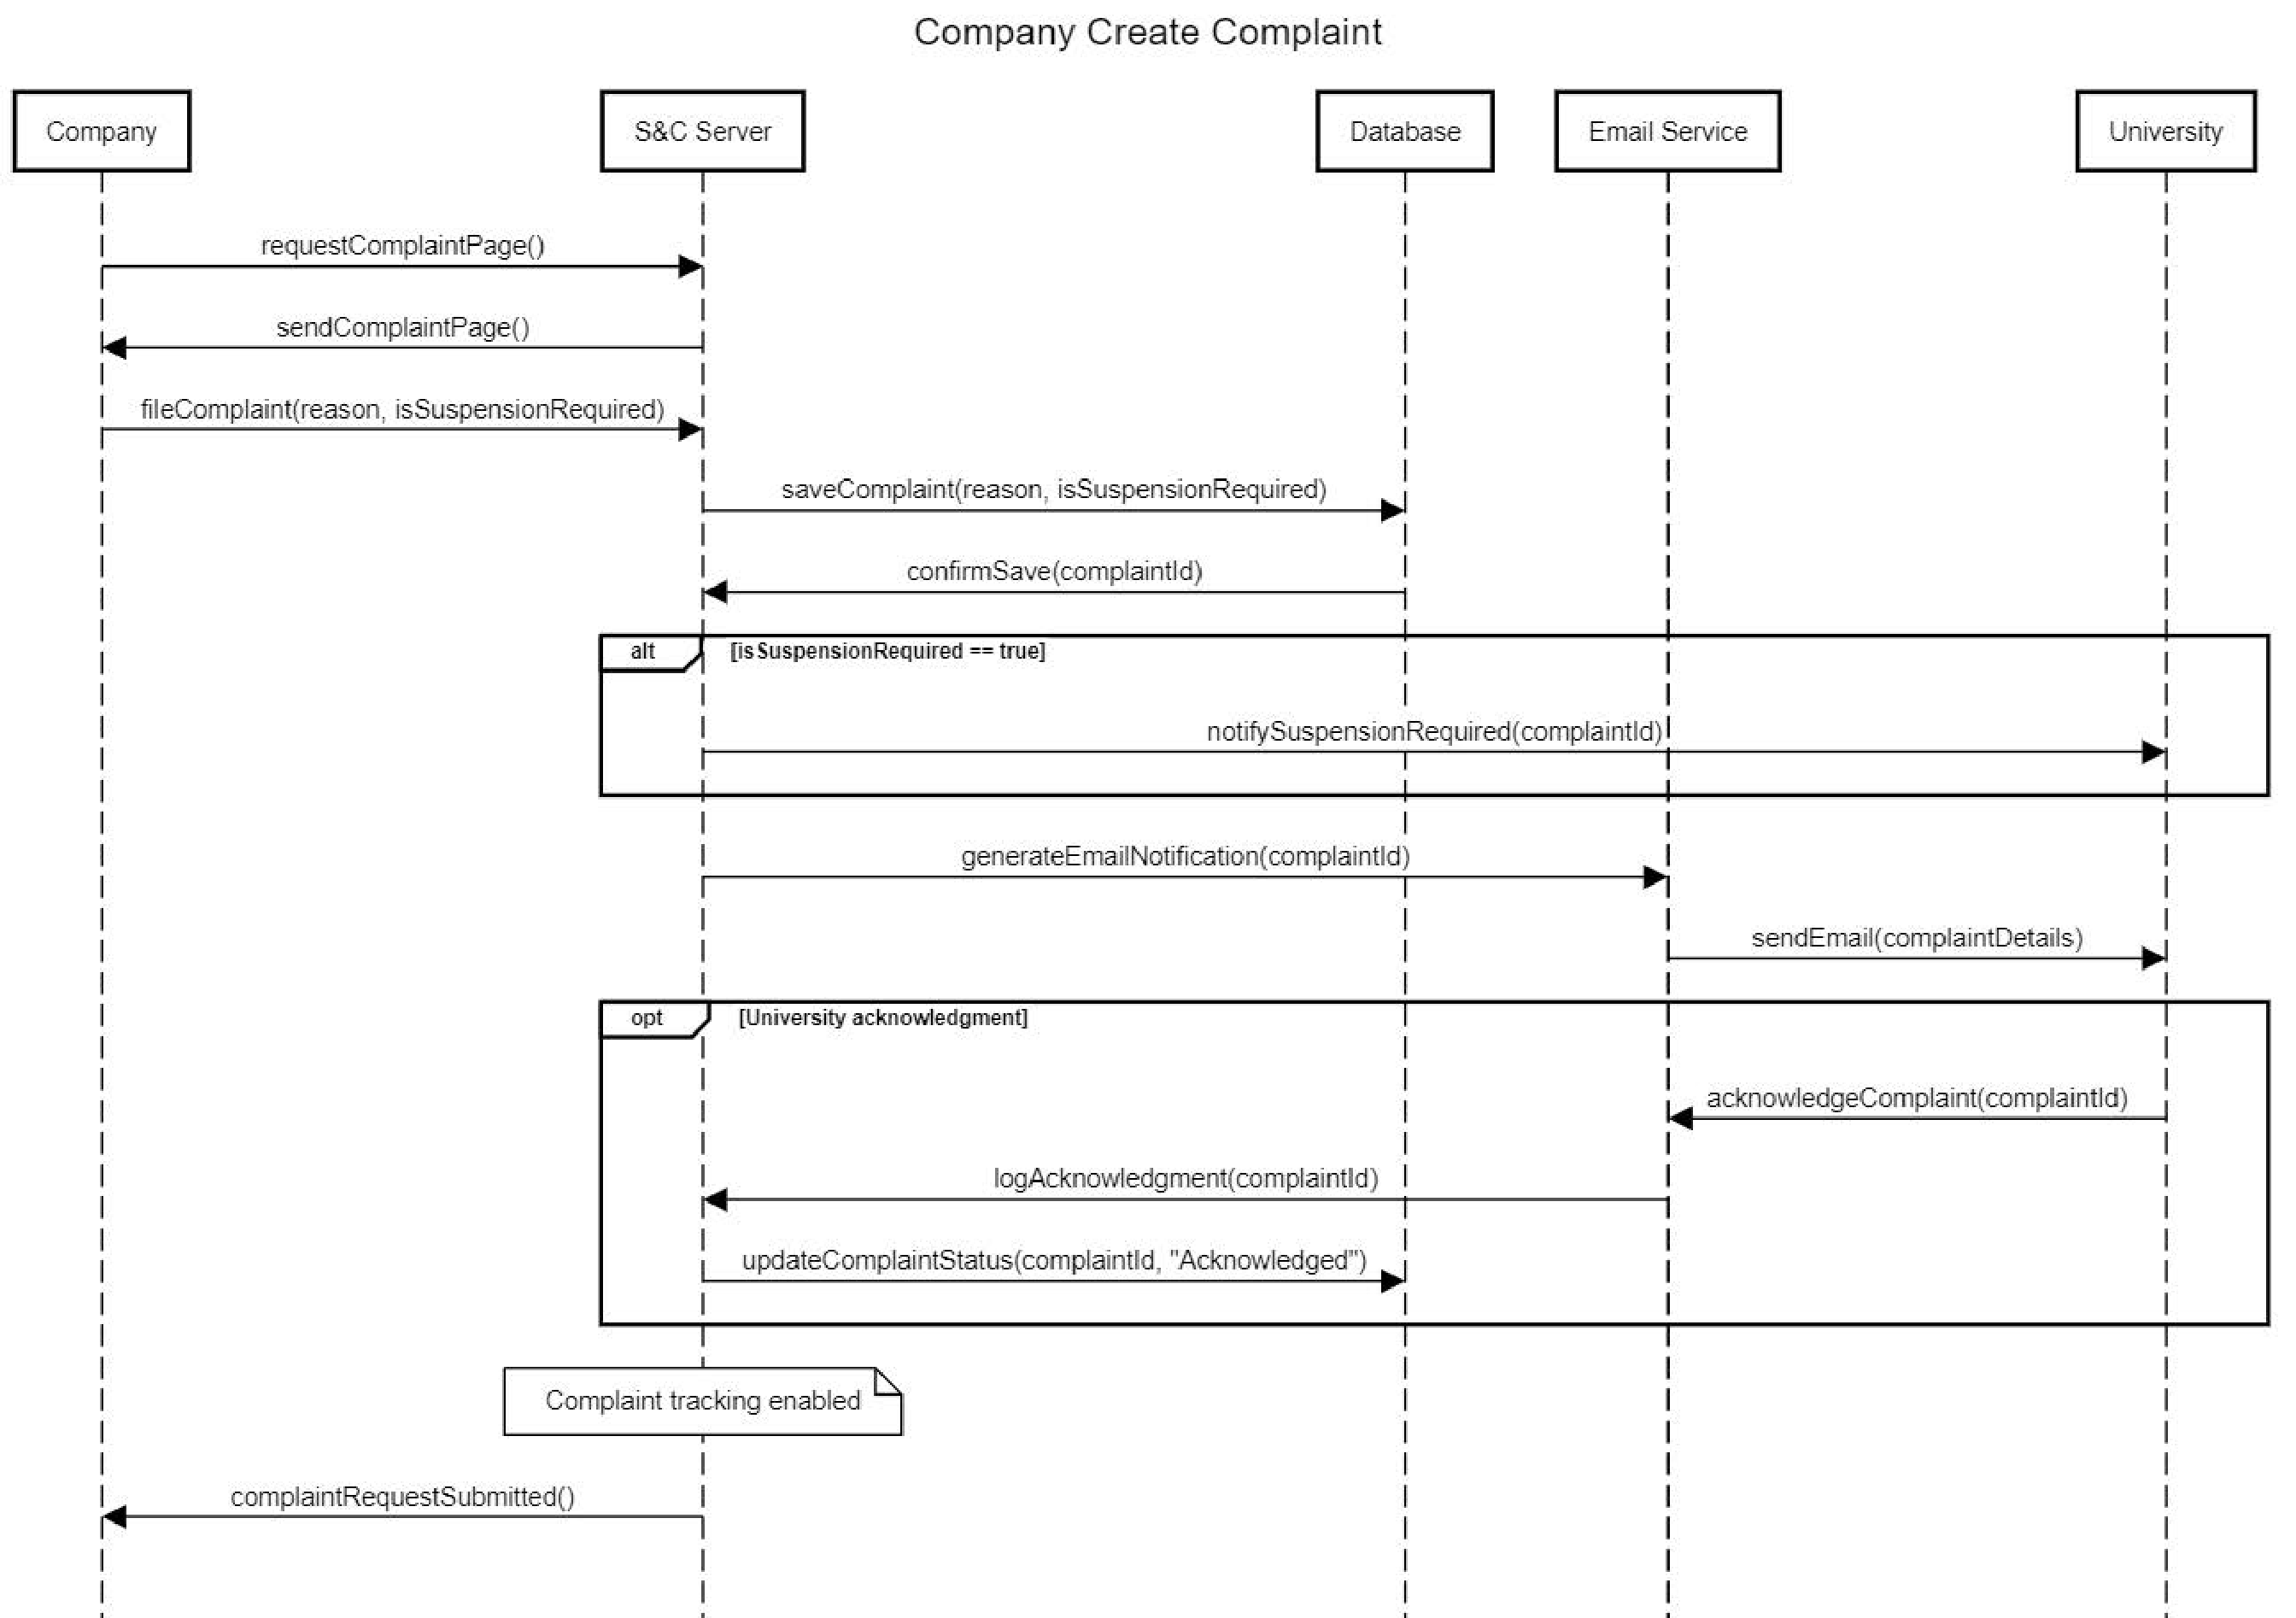
\includegraphics[width=1.0\textwidth]{Images/UC_13.pdf}
    \caption{Company Creates a Complaint - Use Case Diagram}
    \label{fig:use-case-diagram-13}
\end{figure}

% 14

\subsubsection{UC14: Company answers questionnaire at internship completion}
\label{subsubsec:company-answers-questionnaire-at-internship-completion}

\begin{center}
    \begin{longtable}{|l|p{0.75\linewidth}|}
        \hline
        \textbf{Actors:}           & CO                                                                                                                                                        \\
        \hline
        \textbf{Entry Conditions:} & CO is correctly logged in. The internship has ended. CO has received a notification to fill the questionnaire.                                            \\
        \hline
        \textbf{Flow of Events:}   & \begin{enumerate}
                                         \item CO clicks on the "Fill Questionnaire" button.
                                         \item S\&C fetch the questionnaire from the database.
                                         \item S\&C shows the questionnaire to the CO.
                                         \item CO fills each question and submits it.
                                         \item S\&C stores the questionnaire in the database.
                                         \item S\&C notifies the UN that the questionnaire was successfully submitted.
                                         \item S\&C feeds the answers of the questionnaire to the suggestion system to improve it's response on how to improve a CV or an internship advertisement.
                                     \end{enumerate} \\
        \hline
        \textbf{Exit Conditions:}  & CO receive the confirmation of the questionnaire being saved correctly                                                                                    \\
        \hline
        \textbf{Exceptions:}       & S\&C generated an internal error.                                                                                                                         \\
        \hline
    \end{longtable}
\end{center}

\begin{figure}[H]
    \centering
    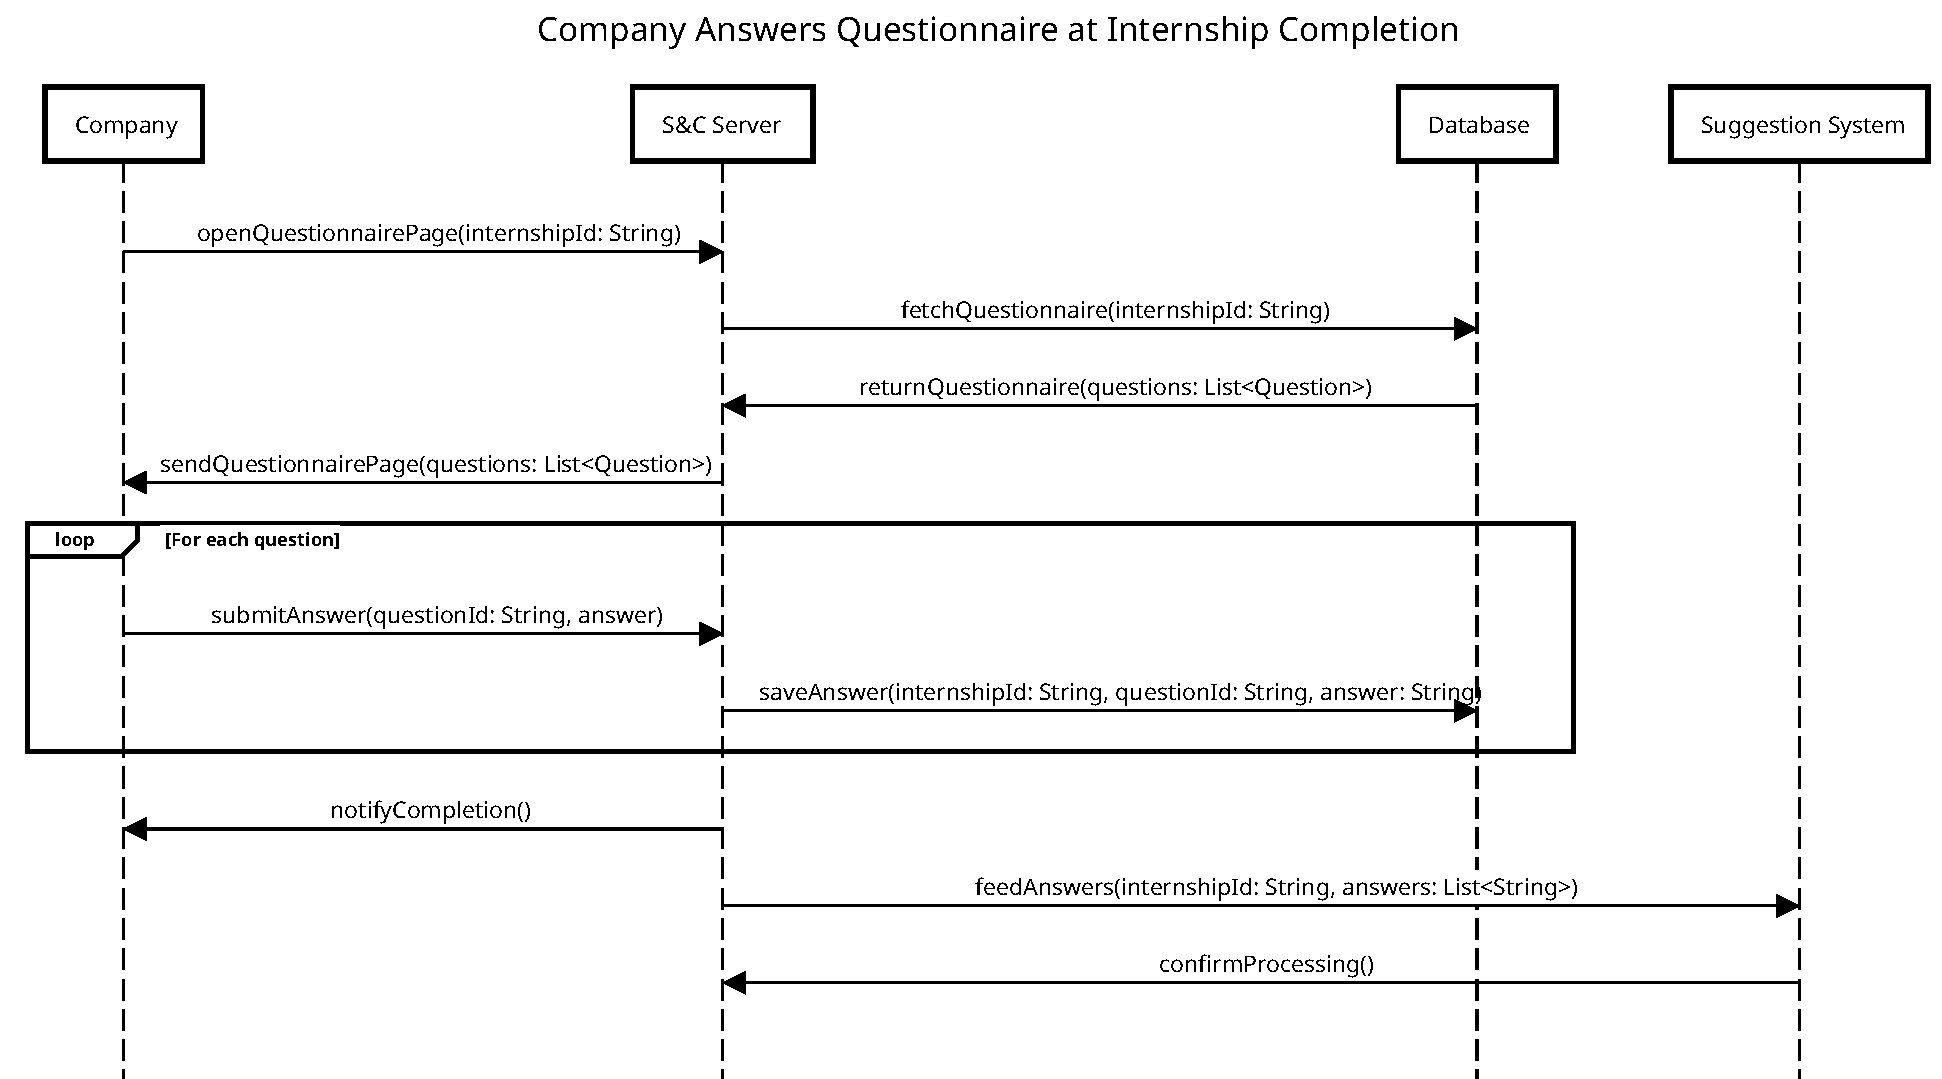
\includegraphics[width=1.0\textwidth]{Images/UC_14.pdf}
    \caption{Company Answers Questionnaire at Internship Completion - Use Case Diagram}
    \label{fig:use-case-diagram-14}
\end{figure}

\pagebreak

% 15

\subsubsection{UC15: Company decides who to hire for an internship}
\label{subsubsec:company-decides-who-to-hire-for-an-internship}

\begin{center}
    \begin{longtable}{|l|p{0.75\linewidth}|}
        \hline
        \textbf{Actors:}           & CO, ST                                                                                  \\
        \hline
        \textbf{Entry Conditions:} & CO is correctly logged in. CO has published an internship listing.                      \\
        \hline
        \textbf{Flow of Events:}   & \begin{enumerate}
                                         \item CO selects an internship to view the details of.
                                         \item S\&C fetch the internship details from the database.
                                         \item S\&C shows the internship details to the CO.
                                         \item CO clicks on the "Applicants" button.
                                         \item S\&C fetch the applicants from the database.
                                         \item S\&C shows the applicants to the CO.
                                         \item CO selects "Show Questionnaires Results" button.
                                         \item S\&C fetch the questionnaires results from the database.
                                         \item S\&C shows the questionnaires results to the CO.
                                         \item CO evaluates the candidates profiles:
                                               \begin{enumerate}
                      \item CO clicks on the "Details" button next to a candidate.
                      \item S\&C fetch the candidate details from the database.
                      \item S\&C fetch the candidate questionnaire answers from the database.
                      \item S\&C shows the candidate details and questionnaire answers to the CO.
                  \end{enumerate}
                                         \item CO decides who to interview and contacts them. At the end, CO decides who to hire.
                                         \item CO clicks on the "Hire" button next to the candidate.
                                         \item S\&C stores the hiring decision in the database.
                                         \item S\&C changes the status of the internship to "On-Going".
                                     \end{enumerate} \\
        \hline
        \textbf{Exit Conditions:}  & CO has successfully hired a candidate for the internship.                               \\
        \hline
        \textbf{Exceptions:}       & S\&C generated an internal error.                                                       \\
        \hline
    \end{longtable}
\end{center}

\begin{figure}[H]
    \centering
    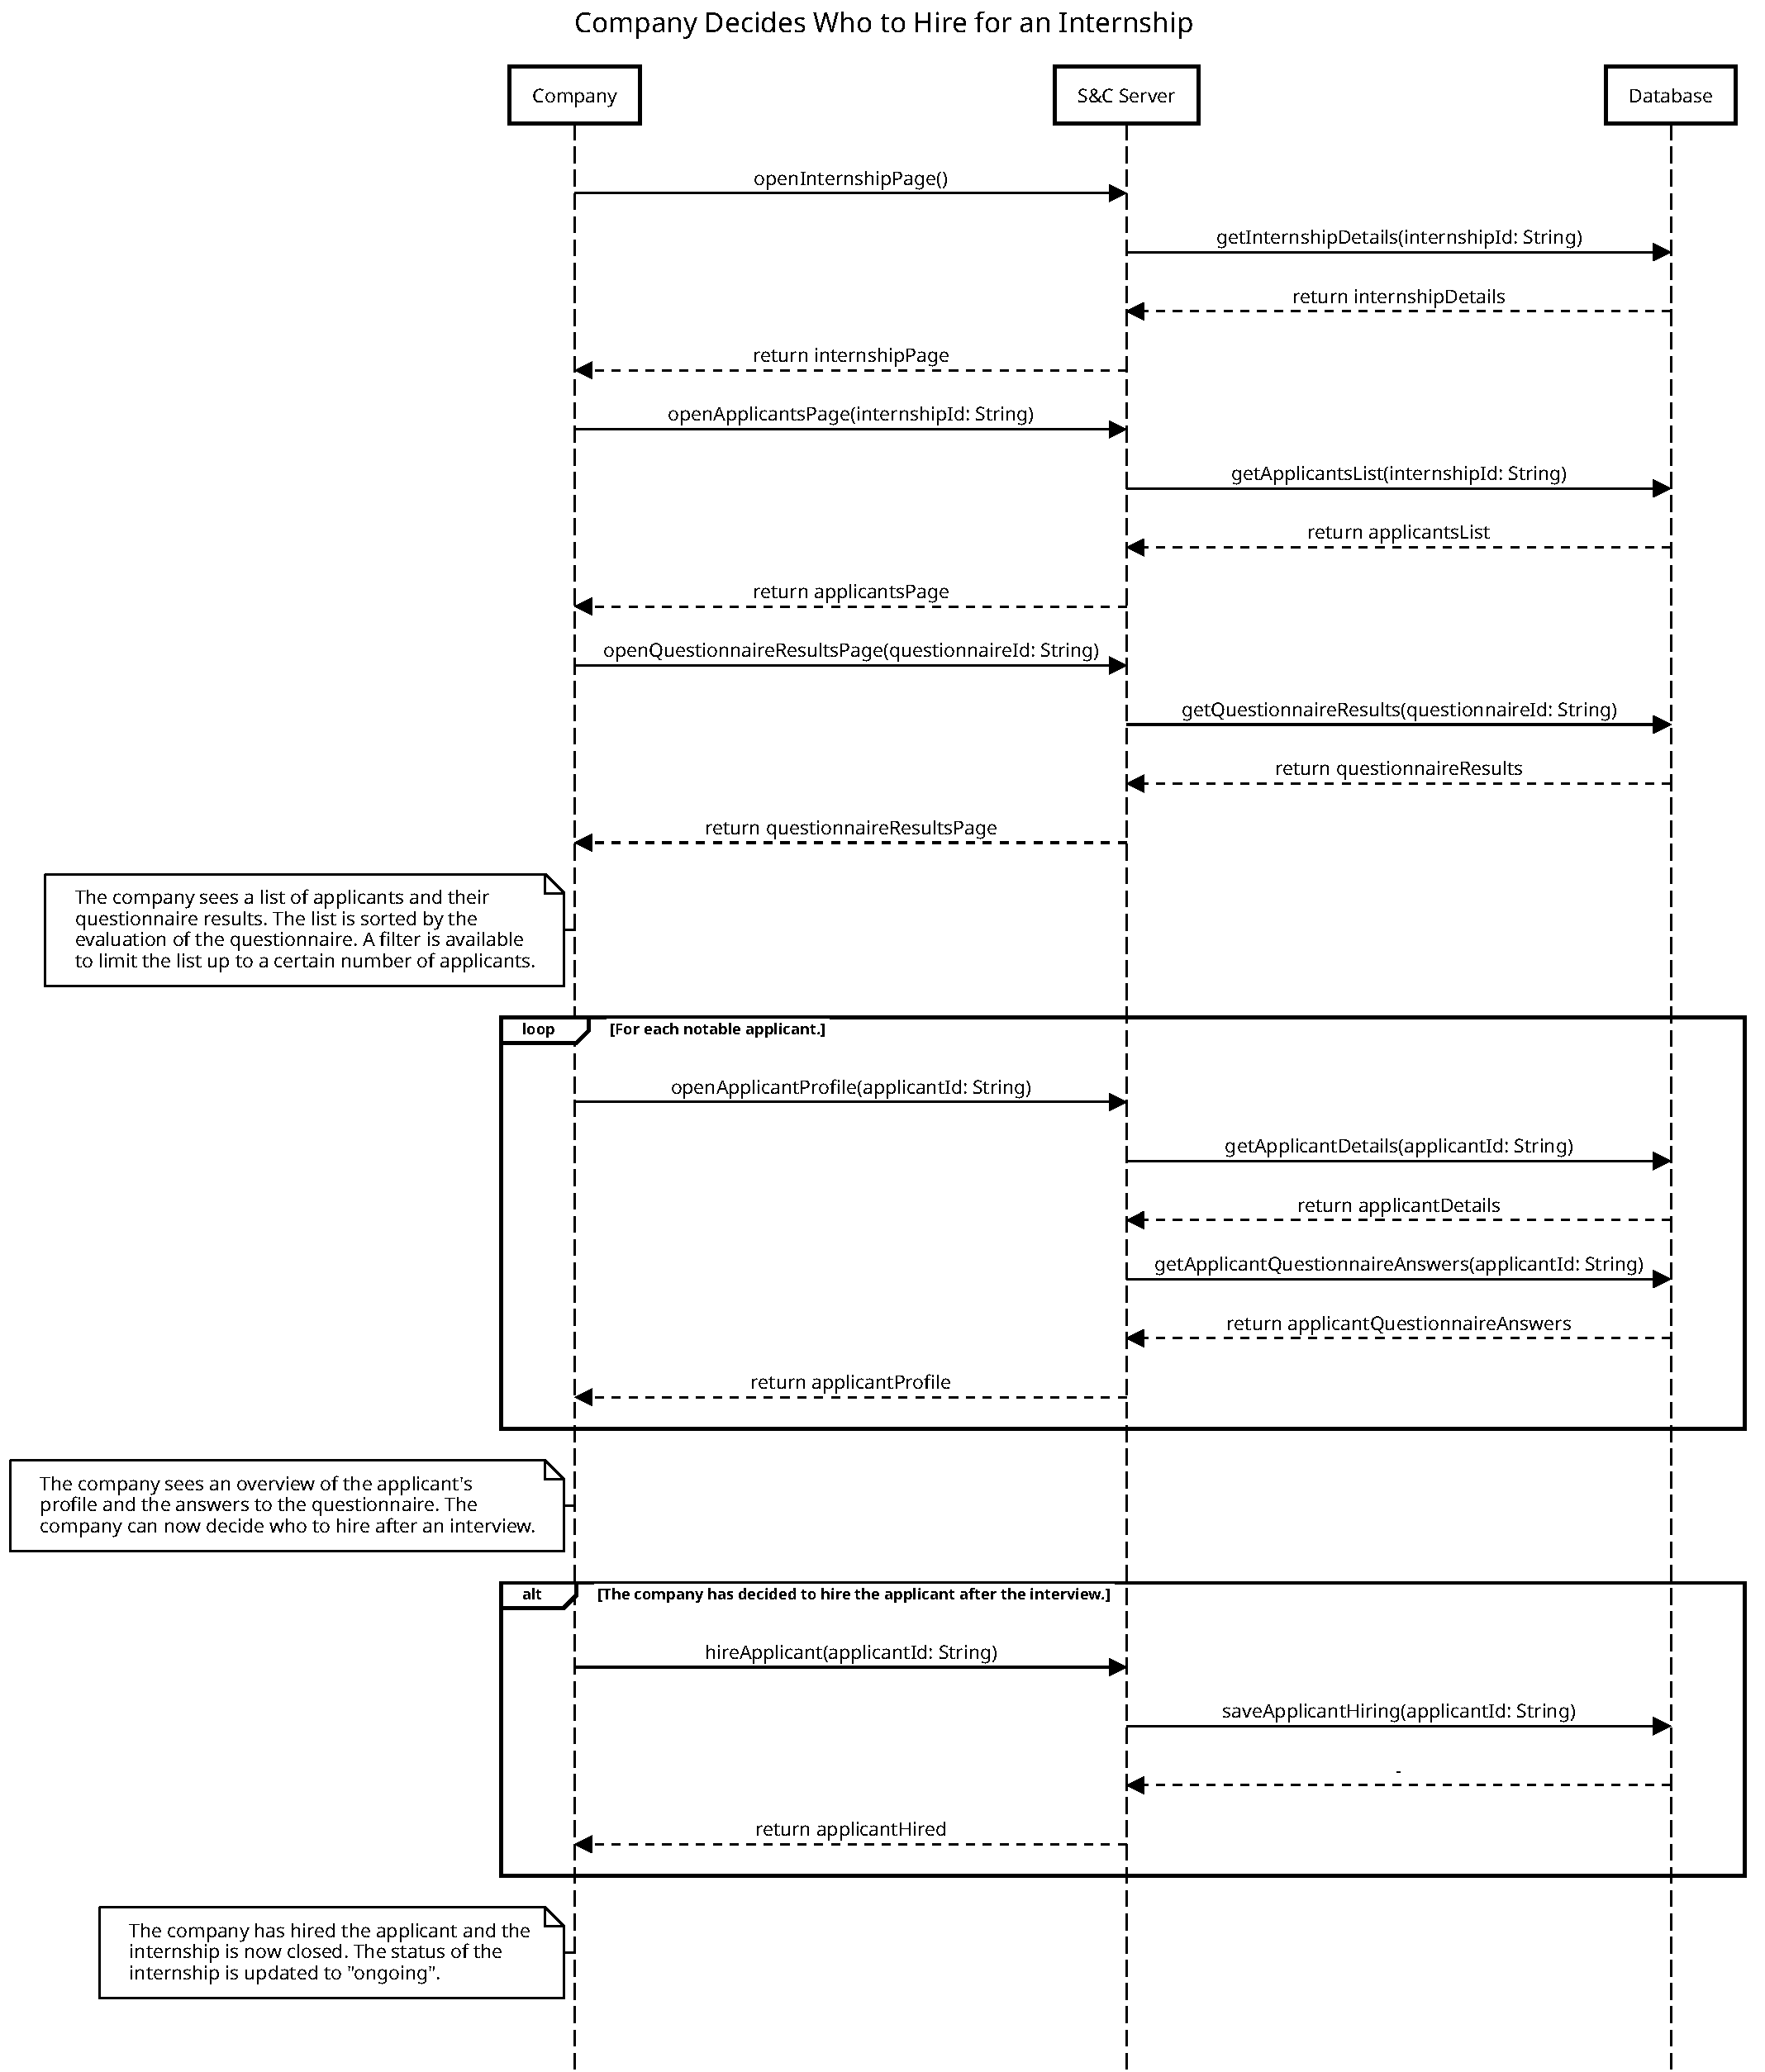
\includegraphics[width=1.0\textwidth]{Images/UC_14A.pdf}
    \caption{Company Decides Who to Hire for an Internship - Use Case Diagram}
    \label{fig:use-case-diagram-15}
\end{figure}

% 16

\subsubsection{UC16: University views the status of the internships}
\label{subsubsec:university-views-the-status-of-the-internships}

\begin{center}
    \begin{longtable}{|l|p{0.75\linewidth}|}
        \hline
        \textbf{Actors:}           & UN                                                          \\
        \hline
        \textbf{Entry Conditions:} & UN is correctly logged in.                                  \\
        \hline
        \textbf{Flow of Events:}   & \begin{enumerate}
                                         \item UN visits the "My Internships" page.
                                         \item S\&C fetches the internships from the database.
                                         \item S\&C shows the internships to the UN.
                                         \item UN filters the internships by keyword, company, etc.
                                         \item S\&C shows the filtered internships to the UN.
                                         \item UN selects an internship to view the details.
                                         \item S\&C fetches the internship details from the database.
                                         \item S\&C shows the internship details to the UN.
                                     \end{enumerate} \\
        \hline
        \textbf{Exit Conditions:}  & UN has successfully viewed the internships of its STs.      \\
        \hline
        \textbf{Exceptions:}       & S\&C generated an internal error.                           \\
        \hline
    \end{longtable}
\end{center}

\begin{figure}[H]
    \centering
    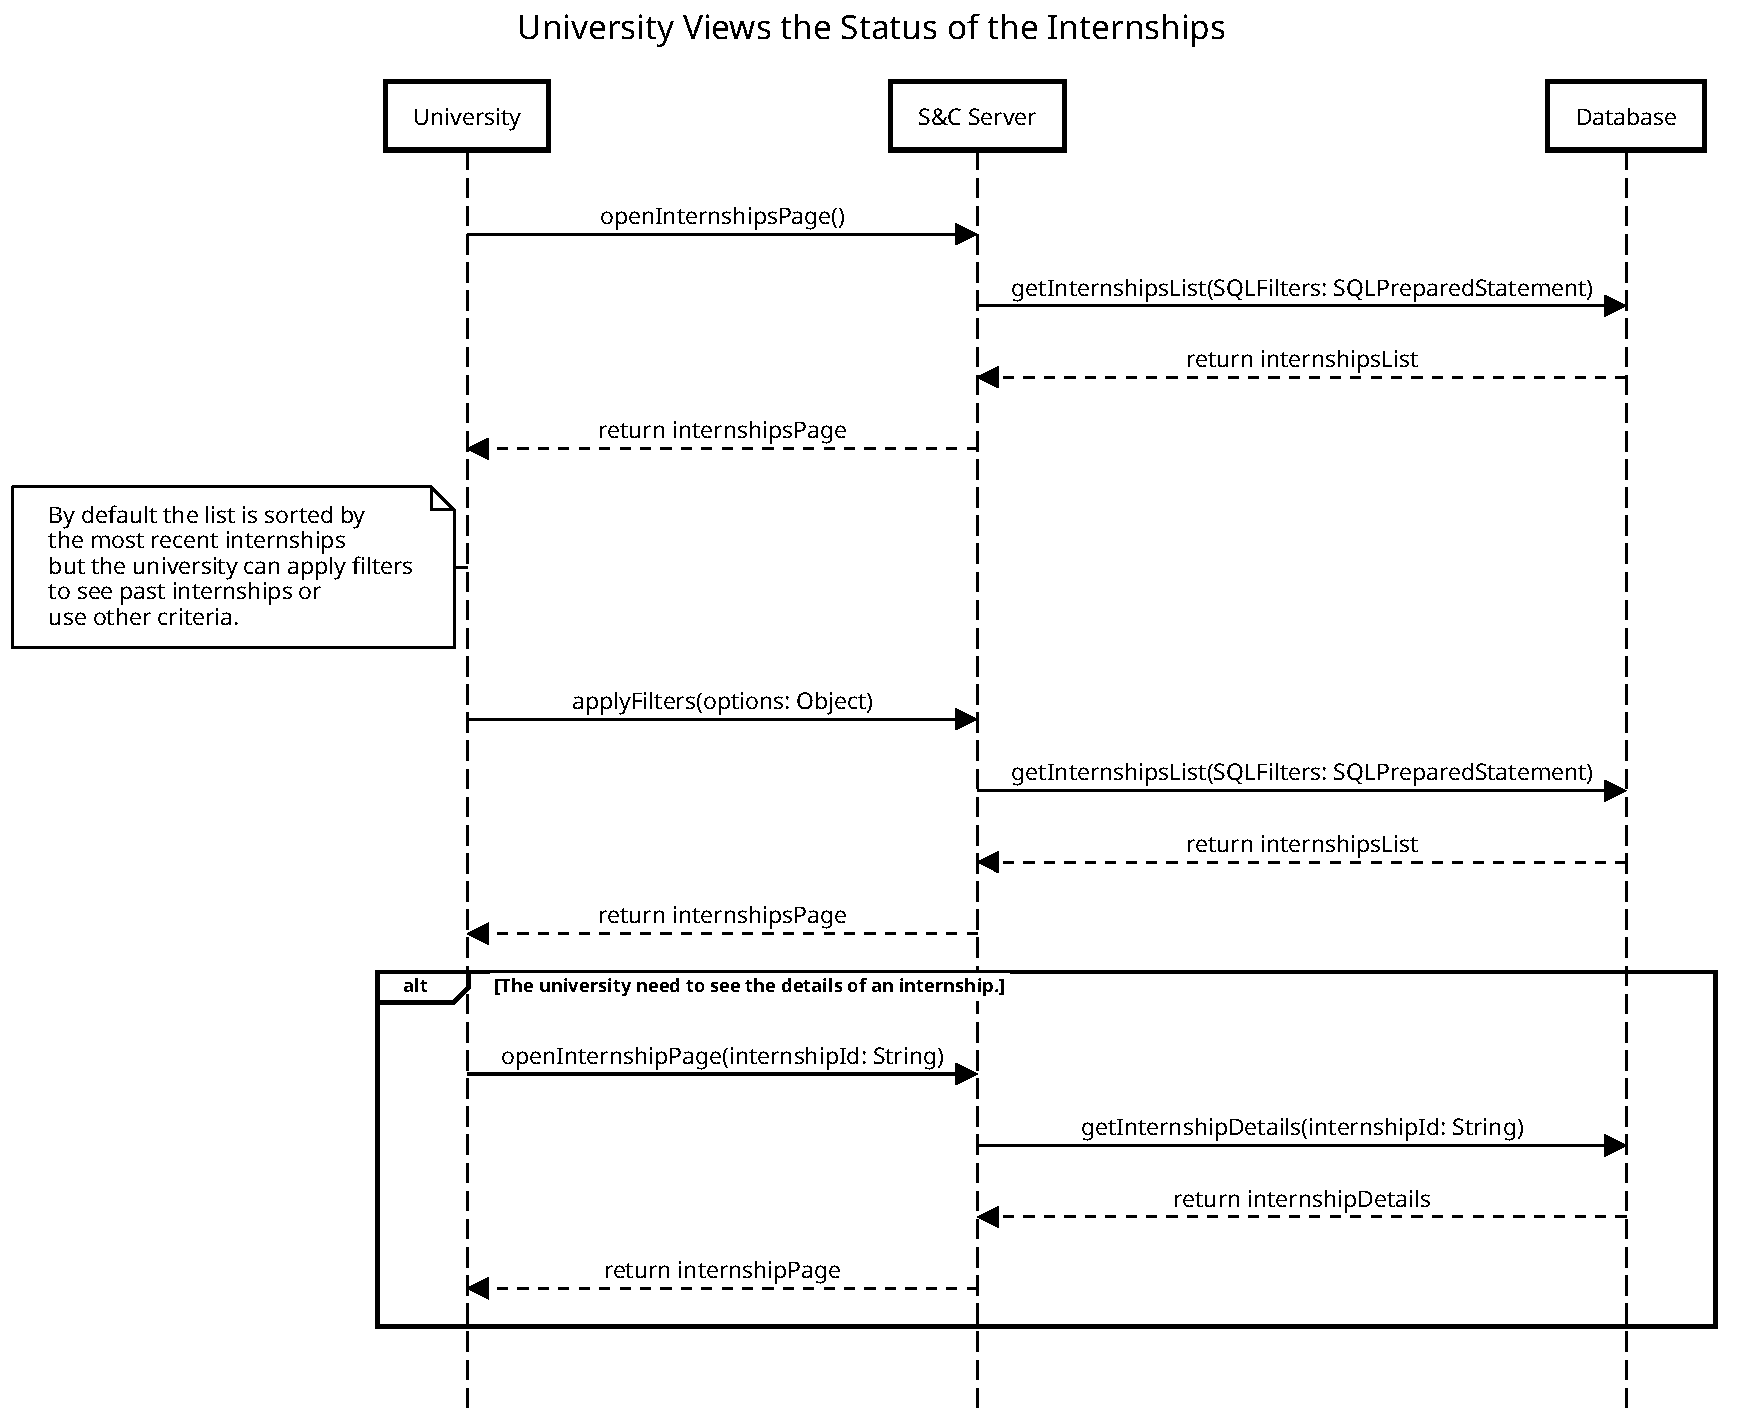
\includegraphics[width=1.0\textwidth]{Images/UC_15.pdf}
    \caption{University Views the Status of the Internships - Use Case Diagram}
    \label{fig:use-case-diagram-16}
\end{figure}

% 17

\subsubsection{UC17: University reviews and handles a complaint}
\label{subsubsec:university-reviews-and-handles-a-complaint}

\begin{center}
    \begin{longtable}{|l|p{0.75\linewidth}|}
        \hline
        \textbf{Actors:}           & UN                                                                                                    \\
        \hline
        \textbf{Entry Conditions:} & UN is correctly logged in. The UN has a list of complaints to review.                                 \\
        \hline
        \textbf{Flow of Events:}   & \begin{enumerate}
                                         \item UN clicks on the "Complaints" button.
                                         \item S\&C fetch the complaints from the database.
                                         \item S\&C shows a preview of the complaints to the UN.
                                         \item UN selects a complaint to review.
                                         \item S\&C fetch the complaint details from the database.
                                         \item S\&C shows the complaint details to the UN.
                                         \item UN review the complaint and writes a response and decide if the internship need to be suspended.
                                         \item S\&C update the status of the complaint with the UN response.
                                         \item S\&C suspend the internship if the UN decided to do so.
                                         \item S\&C notifies the UN that the complaint was successfully reviewed.
                                     \end{enumerate} \\
        \hline
        \textbf{Exit Conditions:}  & UN receive the confirmation of the complaint being reviewed correctly.                                \\
        \hline
        \textbf{Exceptions:}       & S\&C generated an internal error.                                                                     \\
        \hline
    \end{longtable}
\end{center}

\begin{figure}[H]
    \centering
    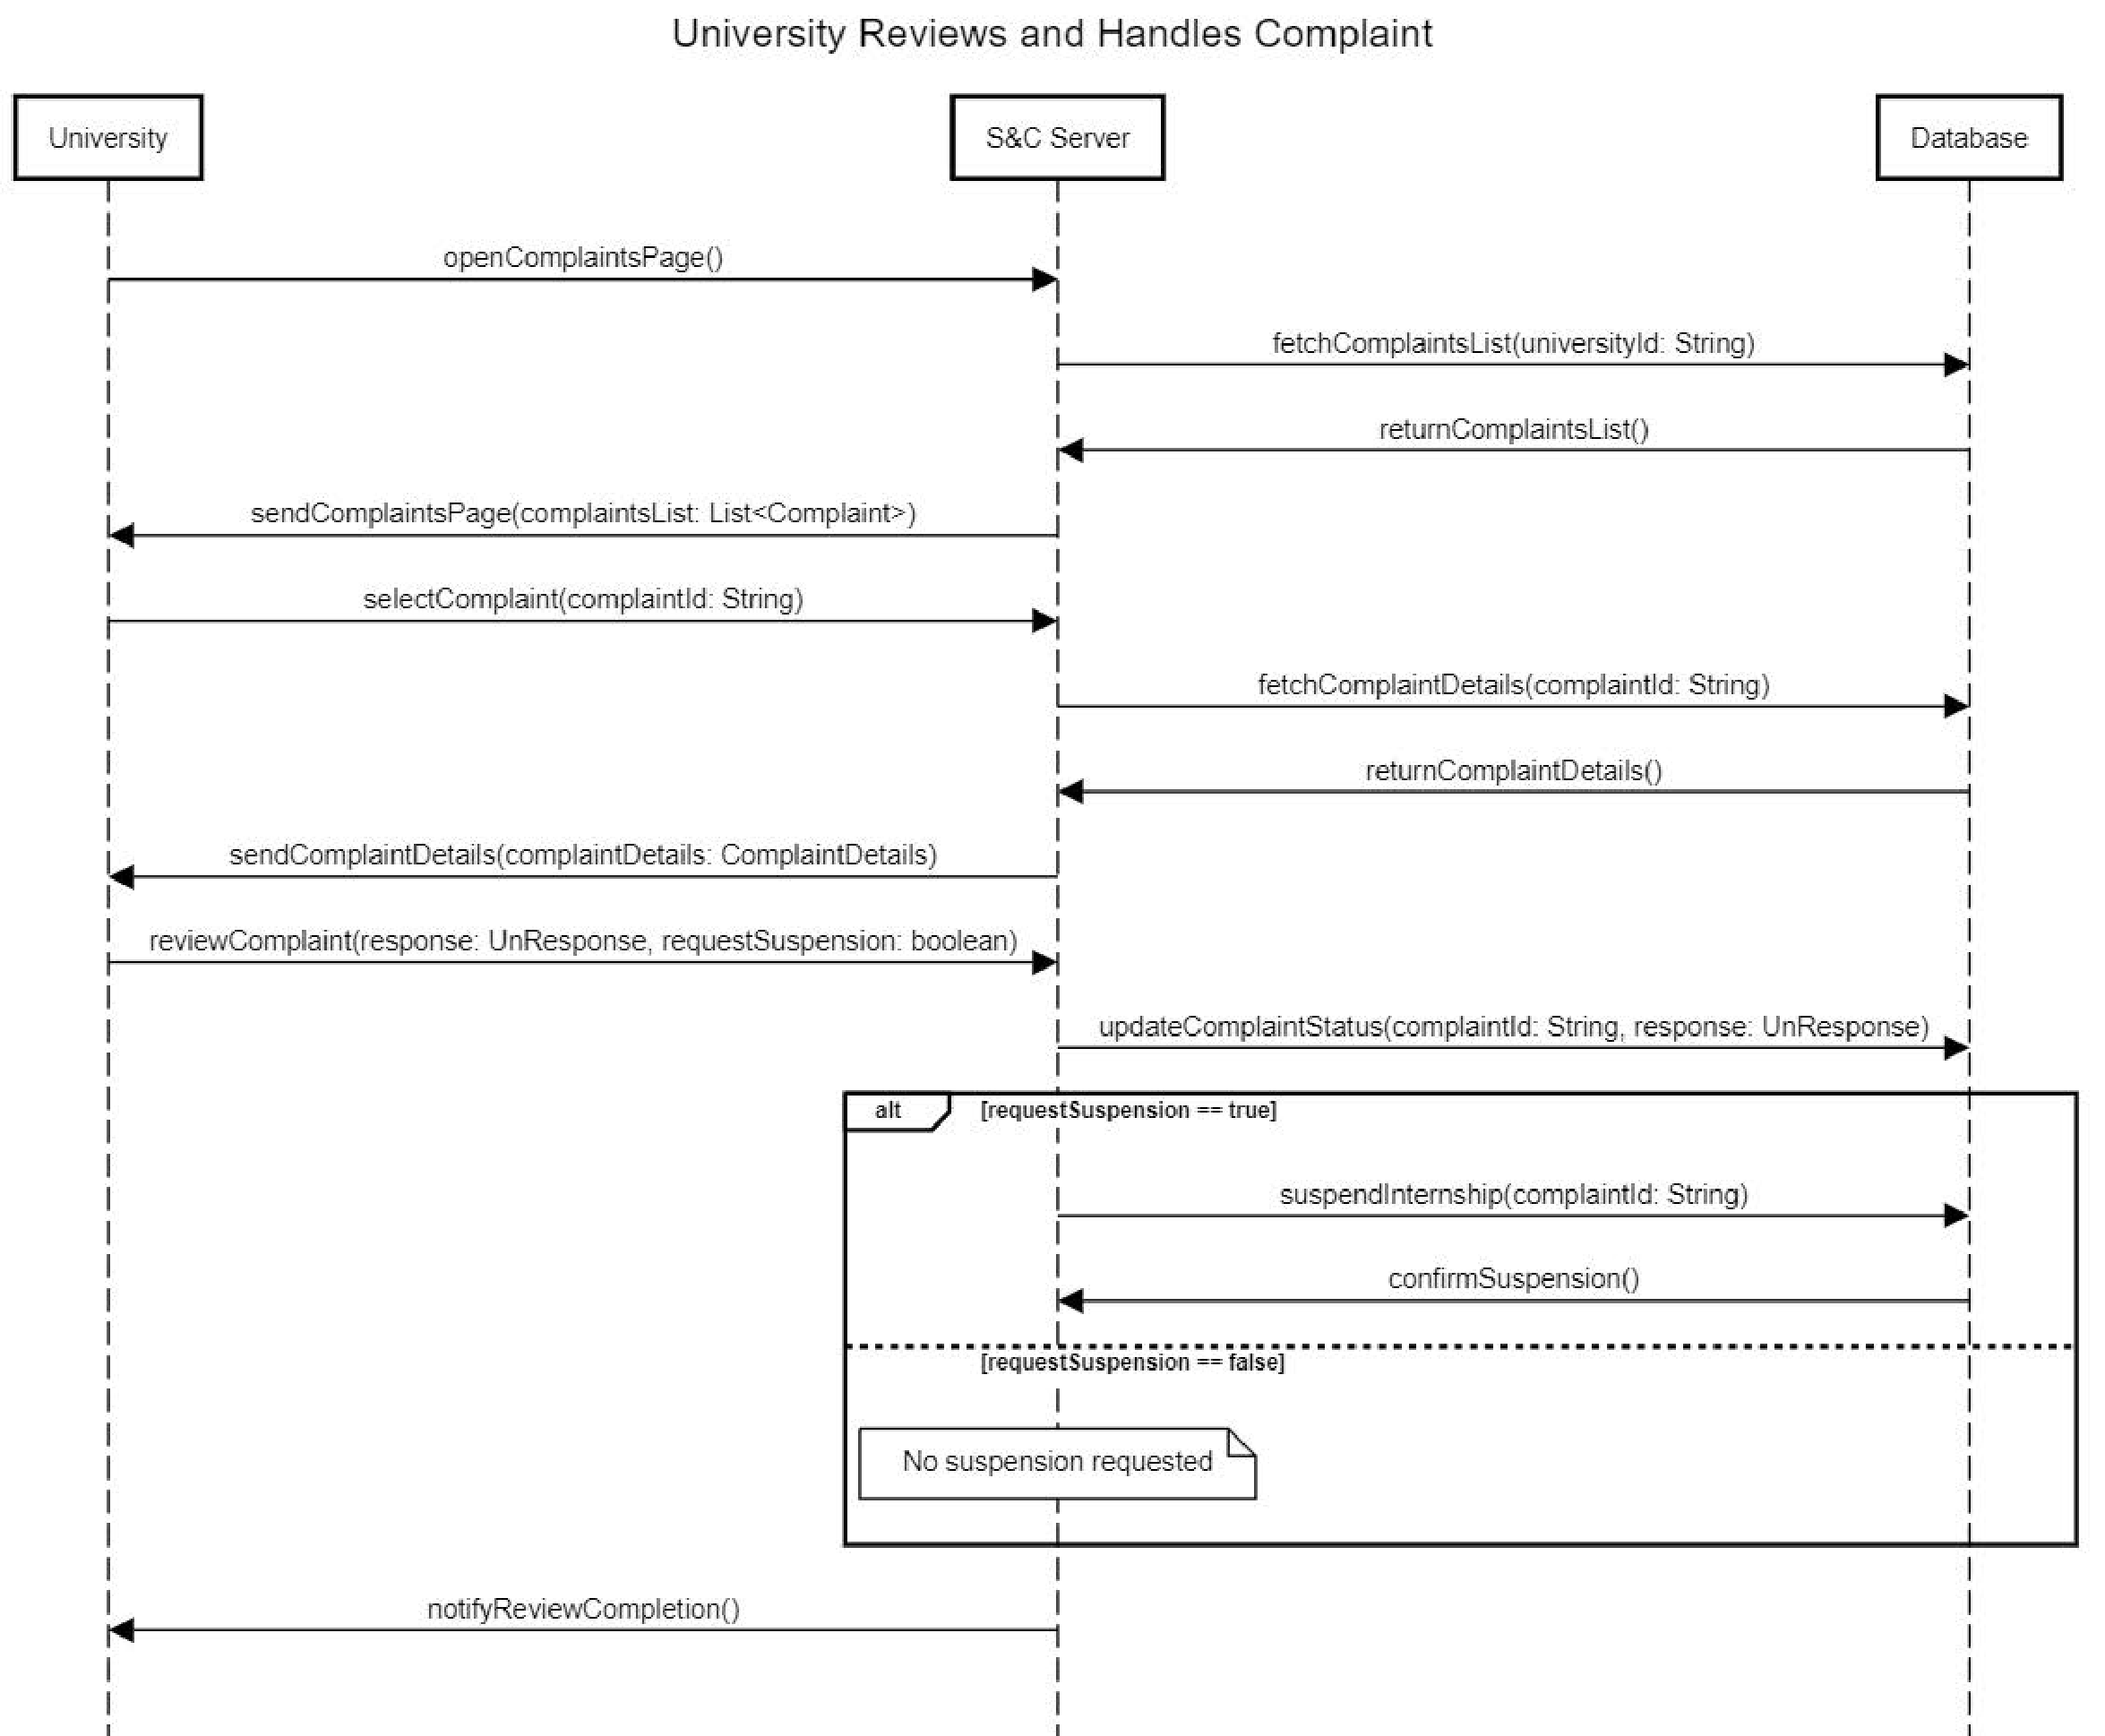
\includegraphics[width=1.0\textwidth]{Images/UC_16.pdf}
    \caption{University Reviews and Handles a Complaint - Use Case Diagram}
    \label{fig:use-case-diagram-17}
\end{figure}

% 18

\subsubsection{UC18: University blocks a malicious company}
\label{subsubsec:university-blocks-a-malicious-company}

\begin{center}
    \begin{longtable}{|l|p{0.75\linewidth}|}
        \hline
        \textbf{Actors:}           & UN                                                                                                            \\
        \hline
        \textbf{Entry Conditions:} & UN is correctly logged in and it has received a serious complaint that requires the blocks of a malicious CO. \\
        \hline
        \textbf{Flow of Events:}   & \begin{enumerate}
                                         \item UN visits the "My Contract" page.
                                         \item S\&C fetches the agreement between UN and corporate.
                                         \item S\&C shows the legal documents currently effective between UN and S\&C corp.
                                         \item UN clicks on "Block a Company" and enters the CO id (ex. P.IVA) of the malicious company.
                                         \item S\&C updates the UN's blacklist adding the specified CO.
                                         \item S\&C shows the user a confirmation.
                                     \end{enumerate}                \\
        \hline
        \textbf{Exit Conditions:}  & UN has now successfully "burnt all the bridges" between its STs and the affected CO.                          \\
        \hline
        \textbf{Exceptions:}       & S\&C generated an internal error. Invalid CO's identifier.                                                    \\
        \hline
    \end{longtable}
\end{center}

\begin{figure}[H]
    \centering
    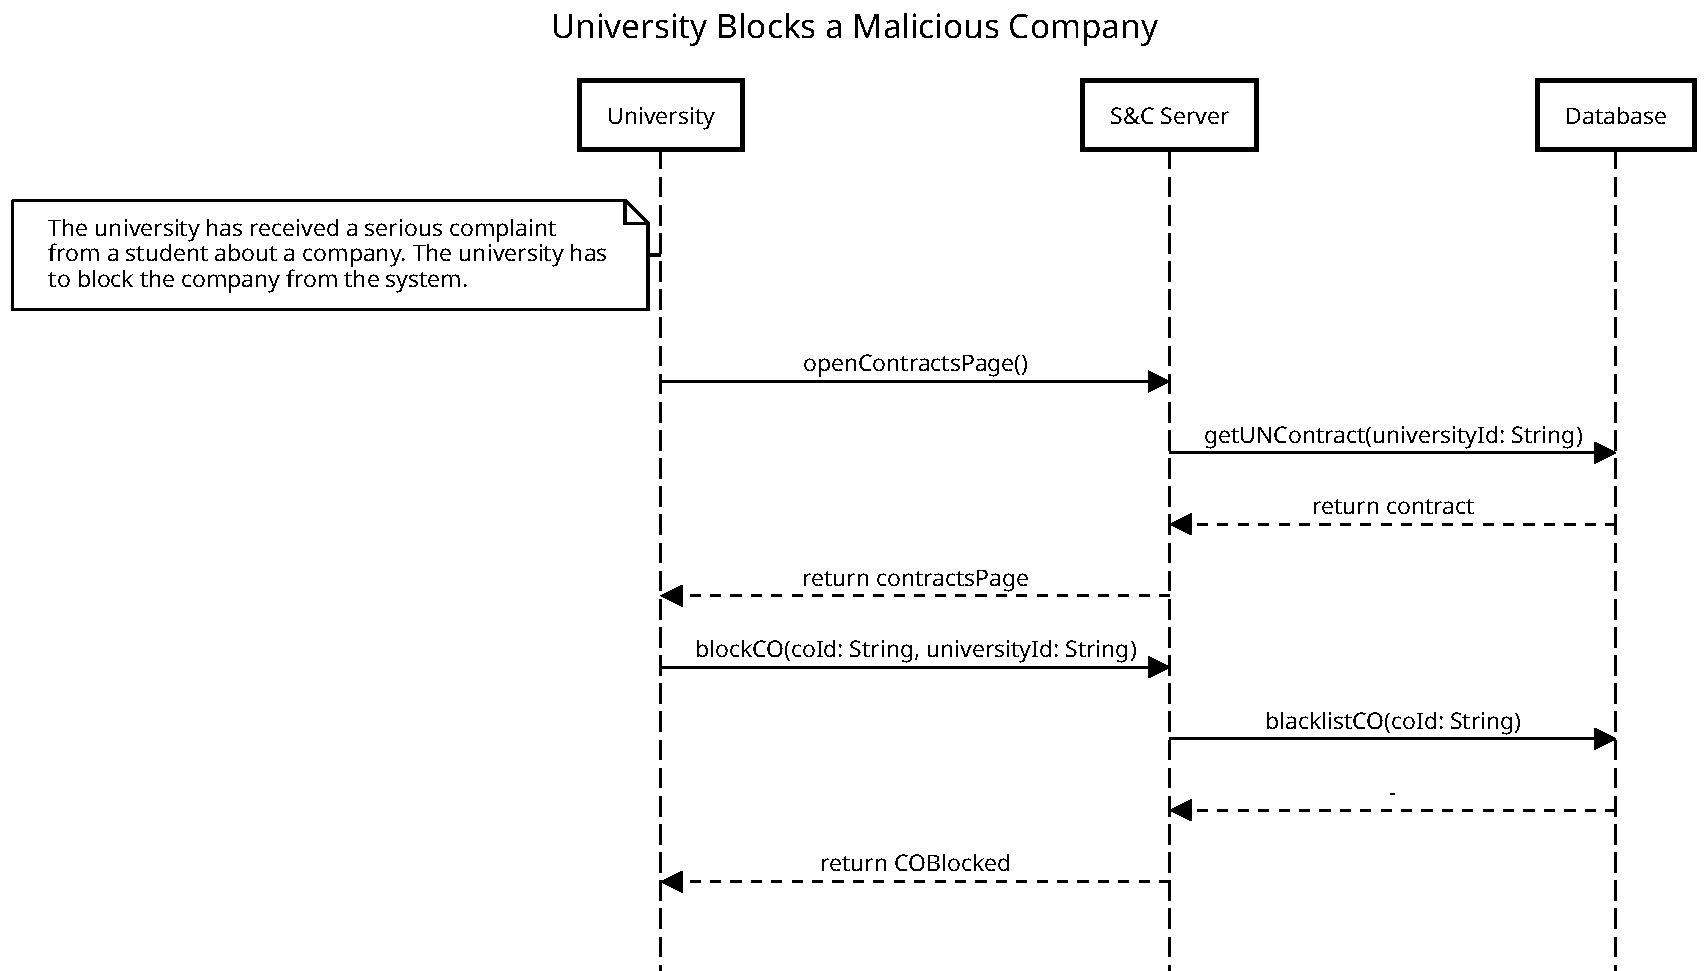
\includegraphics[width=1.0\textwidth]{Images/UC_17.pdf}
    \caption{University Blocks a Malicious Company - Use Case Diagram}
    \label{fig:use-case-diagram-18}
\end{figure}

\subsection{Goals - Requirements Mapping}

The following table shows the mapping between the goals of S\&C (as defined in \ref{tab:goals}, pag. \pageref{tab:goals})
and the system requirements (as defined in \ref{tab:requirements-table}, pag. \pageref{tab:requirements-table}). Goals
and requirements are enumerated by their respective IDs.

% We will now make the following pages landscape to fit the table
\afterpage{%
    \clearpage% Flush earlier floats (otherwise order might not be correct)
    \begin{landscape}% Landscape page
        \centering % Center table
        \begin{longtable}{|l|l|l|l|l|l|l|l|l|l|l|l|l|l|l|l|l|l|l|l|l|l|l|l|l|}
            \hline
            \textbf{$\bm{G_{i}}$ \textrightarrow{}} & \textbf{01} & \textbf{02} & \textbf{03} & \textbf{04} & \textbf{05} & \textbf{06} & \textbf{07} & \textbf{08} & \textbf{09} & \textbf{10} & \textbf{11} & \textbf{12} & \textbf{13} & \textbf{14} & \textbf{15} & \textbf{16} & \textbf{17} & \textbf{18} & \textbf{19} & \textbf{20} & \textbf{21} & \textbf{22} & \textbf{23} & \textbf{24} \\ \hline
            \textbf{R01}                            & \checkmark  &             &             &             &             &             &             &             &             &             &             &             &             &             &             &             &             &             &             &             &             & \checkmark  &             &             \\ \hline
            \textbf{R02}                            &             &             &             &             &             &             &             &             &             &             &             &             &             &             &             &             &             &             &             &             &             & \checkmark  &             &             \\ \hline
            \textbf{R03}                            &             &             &             &             &             &             &             &             &             &             &             & \checkmark  &             &             &             &             &             &             &             &             &             &             &             &             \\ \hline
            \textbf{R04}                            & \checkmark  &             &             &             &             &             &             &             &             &             &             &             &             &             &             &             &             &             &             &             &             &             &             &             \\ \hline
            \textbf{R05}                            & \checkmark  &             &             &             &             &             &             &             &             &             &             &             &             &             &             &             &             &             &             &             &             &             &             &             \\ \hline
            \textbf{R06}                            &             &             &             &             &             &             &             &             &             &             &             & \checkmark  &             &             &             &             &             &             &             &             &             &             &             &             \\ \hline
            \textbf{R07}                            &             &             &             &             &             &             &             &             &             &             &             &             &             &             &             &             &             &             &             &             &             & \checkmark  &             &             \\ \hline
            \textbf{R08}                            &             & \checkmark  &             &             &             &             &             &             &             &             &             &             &             &             &             &             &             &             &             &             &             &             &             &             \\ \hline
            \textbf{R09}                            &             &             &             &             &             &             &             &             &             & \checkmark  &             &             &             &             &             &             &             &             &             &             &             &             &             &             \\ \hline
            \textbf{R10}                            &             &             & \checkmark  &             &             &             &             &             &             &             &             &             &             &             &             &             &             &             &             &             &             &             &             & \checkmark  \\ \hline
            \textbf{R11}                            &             &             & \checkmark  &             &             &             &             &             &             &             &             &             &             &             &             &             &             &             &             &             &             &             &             & \checkmark  \\ \hline
            \textbf{R12}                            &             &             & \checkmark  & \checkmark  &             &             &             &             &             &             &             &             &             &             &             &             &             &             &             &             &             &             &             &             \\ \hline
            \textbf{R13}                            &             &             &             & \checkmark  &             &             &             &             &             &             &             &             &             &             &             &             &             &             &             &             &             &             &             &             \\ \hline
            \textbf{R14}                            &             &             & \checkmark  &             &             &             &             &             &             &             &             &             &             &             &             &             &             &             &             &             &             &             &             & \checkmark  \\ \hline
            \textbf{R15}                            &             &             & \checkmark  &             &             &             &             &             &             &             &             &             &             &             &             &             &             &             &             &             &             &             &             & \checkmark  \\ \hline
            \textbf{R16}                            &             &             &             &             & \checkmark  &             &             &             &             &             &             &             &             &             &             &             &             &             &             &             &             &             &             &             \\ \hline
            \textbf{R17}                            &             &             &             &             &             & \checkmark  &             &             &             &             &             &             &             &             &             &             &             &             &             &             &             &             &             &             \\ \hline
            \textbf{R18}                            &             &             &             &             &             & \checkmark  &             &             &             &             &             &             &             &             &             &             &             &             &             &             &             &             &             &             \\ \hline
            \textbf{R19}                            &             &             &             &             &             &             &             & \checkmark  &             &             &             &             &             &             &             &             &             &             &             &             &             &             & \checkmark  &             \\ \hline
            \textbf{R20}                            &             &             &             &             &             &             &             & \checkmark  &             &             &             &             &             &             &             &             &             &             &             &             &             &             &             &             \\ \hline
            \textbf{R21}                            &             &             &             &             &             &             &             &             & \checkmark  &             &             &             &             &             &             &             &             &             &             &             &             &             &             & \checkmark  \\ \hline
            \textbf{R22}                            &             &             &             &             &             &             &             &             &             &             &             &             &             & \checkmark  &             &             &             &             &             &             &             &             &             &             \\ \hline
            \textbf{R23}                            &             &             &             &             &             &             &             &             &             &             &             &             &             & \checkmark  &             &             &             &             &             &             &             &             &             &             \\ \hline
            \textbf{R24}                            &             &             &             &             &             &             &             &             &             &             &             &             &             &             &             &             &             &             &             & \checkmark  &             &             &             &             \\ \hline
            \textbf{R25}                            &             &             &             &             &             &             &             &             &             &             &             &             &             &             & \checkmark  & \checkmark  &             &             &             &             &             &             &             &             \\ \hline
            \textbf{R26}                            &             &             &             &             &             &             &             &             &             &             &             &             &             &             &             & \checkmark  &             &             &             &             &             &             &             &             \\ \hline
            \textbf{R27}                            &             &             &             &             &             &             &             &             &             &             &             &             &             &             &             & \checkmark  &             &             &             &             &             &             &             &             \\ \hline
            \textbf{R28}                            &             &             &             &             &             &             &             &             &             &             &             &             &             &             &             &             & \checkmark  &             &             &             &             &             &             &             \\ \hline
            \textbf{R29}                            &             &             &             &             &             &             &             &             &             &             &             &             &             &             &             &             &             & \checkmark  &             &             &             &             &             &             \\ \hline
            \textbf{R30}                            &             &             &             &             &             &             &             &             &             &             &             &             &             &             &             &             &             &             & \checkmark  &             &             &             & \checkmark  &             \\ \hline
            \textbf{R31}                            &             &             &             &             &             &             &             &             &             &             &             &             &             &             &             &             &             &             & \checkmark  &             & \checkmark  &             &             &             \\ \hline
            \textbf{R32}                            &             &             &             &             &             &             &             &             &             &             &             &             &             &             &             &             &             &             &             &             &             &             &             & \checkmark  \\ \hline
            \textbf{R33}                            &             &             &             &             &             &             &             &             &             &             &             &             &             &             &             &             &             &             &             &             &             &             &             & \checkmark  \\ \hline
            \textbf{R34}                            &             &             &             &             &             &             &             &             &             &             &             &             &             &             &             &             &             &             &             &             &             &             &             & \checkmark  \\ \hline
            \textbf{R35}                            &             &             &             &             &             &             &             &             &             &             &             &             &             &             &             &             &             &             &             &             &             &             &             & \checkmark  \\ \hline
            \textbf{R36}                            &             &             &             &             &             &             &             &             &             &             &             &             &             &             &             &             &             &             &             &             &             &             & \checkmark  &             \\ \hline
            \textbf{R37}                            &             &             &             &             &             &             &             &             &             &             &             &             &             &             &             &             &             &             &             &             &             &             & \checkmark  &             \\ \hline
            \textbf{R38}                            &             &             &             &             &             &             &             & \checkmark  &             &             & \checkmark  &             &             &             &             &             &             &             &             &             &             &             &             &             \\ \hline
            \textbf{R39}                            &             &             &             &             &             &             &             &             &             &             &             &             &             &             &             &             & \checkmark  &             &             &             &             &             &             &             \\ \hline
            \textbf{R40}                            &             &             &             &             &             &             &             &             &             &             &             &             & \checkmark  &             &             &             &             &             &             &             &             &             &             &             \\ \hline
            \textbf{R41}                            &             &             &             &             &             &             &             &             &             &             &             &             &             &             & \checkmark  &             &             &             &             &             &             &             &             &             \\ \hline
            \textbf{R42}                            &             &             &             &             &             &             &             &             &             &             &             &             &             &             & \checkmark  &             &             &             &             &             &             &             &             &             \\ \hline
            \textbf{R43}                            &             &             &             &             &             &             & \checkmark  &             &             &             &             &             &             &             & \checkmark  &             &             &             &             &             &             &             &             &             \\ \hline
            \caption{Goals - Requirements Mapping Table}
            \label{tab:goals-requirements-mapping}
        \end{longtable}
    \end{landscape}
    \clearpage% Flush page
    \pagebreak
}

\section{Performance Requirements}
\label{sec:performance-requirements}%

\par{\textbf{Latency Requirements}} Regarding performance, S\&C should be developed with a very scalable architecture
capable of assuring its user a great QoE (Quality of Experience): in particular, the latency between user’s interaction
and application response should always be less than 300ms (excluding, of course, end-to-end transmission latency not
imputable to S\&C but on the network itself).

\par{\textbf{Storage Requirements}} The system must also be able to store the needed data safely and implement proper
technique of disaster recovery. The data to be stored are mostly text-based, with the most demanding objects being ST’s
CVs and images used in CO’s profiles. An average of 10 MB/user should be maintained – using compression techniques if
necessary – to ensure the scalability of the application itself.

\par{\textbf{Architecture Sizing}} The primary market of S\&C is Italy, where S\&C corp. can establish relationships
with the various universities of the nation. According to 2024’s data in Italy there are 1.9M universities students,
assuming being able to target 20\% of market capacity this would correspond to a user base of 380K users. Designing the
system to accommodate 500k users should be sufficient and should allow for unexpected expansions The infrastructure
will be dynamically scalable, capable of adjusting to accommodate up to twice the monthly average user count, ensuring
long-term flexibility and performance.

\section{Design Constraints}
\label{sec:design-constraints}%

\subsection{Standards Compliance}
\label{subsec:standards-compliance}%

\par S\&C should be compliant with EU’s GDPR regulations to be able to operate in Italy legally ensuring the protection
of the users’ personal data and privacy.

\subsection{Hardware Limitations}
\label{subsec:hardware-limitations}%

\par Server-side, the system must be able to run on commodity x86 hardware. Client-side the requirements are much
blander, only requiring a UE (User Equipment) capable of running a modern web-browser connected with a reliable
connection to the Internet.

\section{Software System Attributes}
\label{sec:software-system-attributes}%

\subsection{Reliability}
\label{subsec:reliability}%

\par The system must be designed in such a way that errors can’t propagate over the whole architecture and fault can be
easily identified and isolated. Enough replicas of data and services should be implemented to ensure the reliability of
the application.

\subsection{Availability}
\label{subsec:availability}%

\par The system must be available 99.99\% (four-nines) of the time, thus allowing 52 minutes of down-time yearly.

\par Maintenance should be carried out when the impact on the clients is negligible and must be announced in advance.

\subsection{Security}
\label{subsec:security}%

\par The system implements a comprehensive authentication and authorization framework to manage user access rights.
Authentication verifies the identity of users attempting to log in, while authorization ensures that authenticated
users possess appropriate permissions for requested actions.

\par To safeguard the system's integrity, standard security measures will be implemented, including encryption of user
credentials and personal data and protection mechanisms against database query injection vulnerabilities.

\subsection{Maintainability}
\label{subsec:maintainability}%

\par The system must be modular enough to allow future expansions with limited effort and repercussion. Enough replicas
of the system must be always up to allow maintenance without impacting on user’s traffic.

\subsection{Portability}
\label{subsec:portability}%

\par As stated before, the server-side architecture must be able to run on commodity x86 hardware and the client-side
frontend must be reachable with a generic browser from the endpoints.


\chapter{Formal Analysis using Alloy}%
\label{chap:Formal-Analysis-using-Alloy}%

\par Here is the formal Analysis and verification of the system proviously described in the RASD document. The analysis is done using the Alloy language and the Alloy Analyzer tool.
The analysis is focused on modeling the temporal evolution and development of an internship.

\section{Alloy Model}%
\label{sec:Alloy-Model}%


\par Here is the Alloy model of the system.

\begin{lstlisting}[language=Alloy]
    
        //actors
        sig Student {
            uni : one University,
            //TODO check internships: one Internship, //internship the student has participated in
            complaints: set Complaint
        }
        
        //company signature
        sig Company {
            
        }
         
        //university signature, carries the information about the blocked companies
        sig University {
            blocked: set Company
        }
        
        //internship signature, carries most of the information about the entire process
        sig Internship {
            var state: one Status,
            var applicants: set Student, //applicants are the students that have applied and will recieve the Interview questionnaire
            var selected_student: lone Student,
            company: one Company,
            questionnaire: one Interview,
            deadline: one Date,
            var responses: set Student, //students that have responded to the Interview questionnaire
            duration: one WorkPeriod,
            feedback: one Feedback
        }
        
        //work period of the internship
        sig WorkPeriod{
            start: one Date,
            end: one Date
        }
        //generic questionnaire
        abstract sig questionnaire{
            
        }
        //interview questionnaire for the selection phase
        sig Interview extends questionnaire{
            
        }
        
        //feedback questionnaire for when the internship is completed without being calcelled
        sig Feedback extends questionnaire{
            var compiled_by: lone Student
        }
        
        sig Complaint{
            submitter: one Student,
            content: one String
        }
        
        //dates 
        sig Date{
            comes_later_than: set Date
        }
        
        
        //statuses for internships
        abstract sig Status{
        
        }
        
        one sig Created, Open, Selecting, Ongoing, Completed, Interrupted, Terminated extends Status{
        
        }
        
        
       
\end{lstlisting}
\par Now the fats that hold on the model.
\begin{lstlisting}[language=Alloy]
            
              
        //the student can't apply to internship if the company is blocked by the university
        fact blocked{
                all i: Internship | all st :i.applicants | i.company not in st.uni.blocked
            }
        
        //the work period starts later than the deadline
        fact breathing_room{
        all i: Internship | later_date[i.duration.start, i.deadline]
        }
        
        //the work period ends later than the start
        fact work_period_start_before_end {
        all wp: WorkPeriod | later_date[wp.end, wp.start]
        }
        
        //each internhips is offered by one company
        fact one_company_per_internship{
        all c1,c2 :Company | (c1 != c2) implies c1.company_internships & c2.company_internships = none
        }
        
        //total ordering on dates
        fact antisymmetry{
                all d1,d2:Date |  d1 in d2.comes_later_than  implies d2 not in d1.comes_later_than
            }
        fact transitivity{
                all d1,d2,d3 :Date | (d1 in d2.comes_later_than and d2 in d3.comes_later_than) implies d1 in d3.comes_later_than
            }
        fact  total_order{
        all  d1, d2 : Date |d1 != d2 implies  ( d1 in d2.comes_later_than or d2  in d1.comes_later_than)
        }
        fact no_reflexivity{
        all d:Date | d not in d.comes_later_than
        }
        
        
        //fact that define the temporal evolution of the internship
        //forces the initial state of every intership to be "Created"
        fact begin{
                always some i: Internship | i.state != Created implies once i.state = Created
            }
        
        
        //temporal evolution of the internship state
        //states represent a snapshot of the intersnhip right before the transition to the next state
        fact evolution{
                always all i:Internship | i.state = Created implies  i.state' = Open
                always all i:Internship | i.state = Open implies  i.state' = Selecting
                always all i:Internship | i.state = Selecting implies  i.state' = Ongoing
                always all i:Internship | i.state = Ongoing implies (i.state' = Completed or i.state' = Interrupted)
                always all i:Internship | i.state = Completed  implies i.state' = Completed
                always all i:Internship | i.state = Interrupted  implies (i.state' = Terminated or i.state' = Ongoing)
                always all i:Internship | i.state = Terminated  implies i.state' = Terminated
            }
        //initial state of the internship
        fact Created_is_uninitialized_state{
        always some i: Internship | i.state = Created implies (i.applicants = none and i.selected_student = none and i.responses = none)
        }
        
        //possible values of variables in states
        fact Open_is_only_for_applying{
        always some i: Internship | i.state = Open implies (i.responses = none and i.selected_student = none and i.applicants != none)
        }
        fact Selecting_is_for_interviews{
        always some i: Internship | i.state = Selecting implies (i.responses != none and i.selected_student = none) //applicants will be none because of persistence
        }
        fact Ongoing_means_selected{
        always some i: Internship | i.state = Ongoing implies i.selected_student != none
        }
        
        //constraints to ensure that variables evolve correctly, at the correct time and no information is lost
        fact responders_are_applicants{
        always all i:Internship | i.responses in i.applicants
        }
        fact Apply_only_when_open{
        always all i:Internship | (i.state != Created ) implies i.applicants = i.applicants' //the only transition that can change the applicants is the one from Created to Open
        }
        fact Respond_only_when_selecting{
        always all i:Internship | (i.state != Open ) implies i.responses = i.responses' //the only transition that can change the responses is the one from Open to Selecting
        }
        fact Select_only_before_Ongoing{
        always all i:Internship | (i.state != Selecting ) implies i.selected_student = i.selected_student' //the only transition that can change the selected_student is the one from Selecting to Ongoing
        }
        //in order to be selected the student must have responded to the interview questionnaire
        fact selected_has_responded{
        always all i: Internship | i.selected_student = none or i.selected_student in i.responses
        }
        
        //feedback is compiled only when the internship is completed
        fact uncompiled_feedback{
        always all i: Internship | i.state != Completed implies i.feedback.compiled_by = none
        }
        
        //if the internship is completed, the feedback must be compiled by someone
        fact feedback_compilation{
        all i: Internship | eventually i.state = Completed implies eventually i.feedback.compiled_by != none
        }
        
        //feedback is compiled by the selected student or by none if the internship is not completed
        fact compiled_by_selected{
        always all i: Internship | i.feedback.compiled_by = i.selected_student or i.feedback.compiled_by = none
        }
        
        //useful assertions ,predicates and functions used in the model and for testing it during development of it.
        
        /d1 is later than d2
        pred later_date[d1,d2: Date]{
        d2 in d1.comes_later_than
        }
        
        //does the university have multiple students?
        pred multiple_students[un:University]{
        #un.University_students > 1
        }
        
        //does the intenship terminate correctly?
        pred normal_development[i:Internship]{
        eventually i.state = Completed
        }
        
        //has the internship been interrupted?
        pred interrupted[i:Internship]{
                eventually i.state = Interrupted
            }
        
        //check the total number of applications recieved
        assert response_cardinality{
        always all i: Internship | #i.applicants >= #i.responses
        }
        
        //check for non emptiness
        assert ongoing_check{
        all i: Internship | i.state = Ongoing implies i.applicants != none and i.responses != none
        }
        
        //no internships gets stuck without a way to progress
        assert process_end{
        eventually all i: Internship | i.state = Completed or i.state = Terminated
        }
        
        //check for valid applicants (students that are not blocked by the company)
        assert valid_applicants{
        all i: Internship | all a: i.applicants | a in Student and i.company not in a.uni.blocked
        }
        
        //check for valid responses (students that are not blocked by the company)
        assert valid_responses{
        all i: Internship | all r: i.responses | r in i.applicants and r in Student and i.company not in r.uni.blocked
        }
        //returns the students of a university
        fun University_students[u:University] : set Student {
                {s:Student | s.uni = u}
            }
        //returns the internships of a company
        fun company_internships[c:Company] : set Internship {
                {i:Internship | i.company = c}
            }
        
\end{lstlisting}

\end{document}


\end{document}